% Information Fusion (Elsevier) build root, 2026-09-28. Fifth venue root
% alongside jair.tex, tmlr.tex, arxiv.tex and iclr2027.tex; the shared body is
% main.tex, as for the others.
%
% Information Fusion is single-anonymized, so the author block is real.
% elsarticle puts title, authors, abstract, highlights and keywords inside
% \begin{frontmatter}; main.tex skips its own title block when
% \FrontmatterAlreadySet is defined.
%
% The xcolor option must be passed before the class for the same reason as in
% every other root: a later [table] request option-clashes silently and
% \cellcolor goes undefined.
\PassOptionsToPackage{table}{xcolor}
\documentclass[preprint,12pt,authoryear]{elsarticle}

\journal{Information Fusion}

% Shared preamble: everything both the ICLR and the arXiv build need.
% Venue-specific bits (documentclass, style file, title block, bib style)
% live in build/iclr2027.tex and build/arxiv.tex.

\usepackage[utf8]{inputenc}
\usepackage[T1]{fontenc}
\usepackage{amsmath,amssymb,amsthm}
\usepackage{enumitem}
\usepackage{graphicx}
\usepackage{booktabs}
\usepackage{multirow}
\usepackage[table]{xcolor}
\usepackage{url}
\usepackage{hyperref}

% Verbatim inclusion of the pre-registration documents in the appendix.
% They are plain text and must appear exactly as committed, so they are
% \lstinputlisting'd from prereg/ rather than retyped: the appendix cannot
% drift from the files, because it is the files. Widest line in the set is
% 85 columns, which fits at \footnotesize, but breaklines is on so that a
% future edit to one of them cannot silently produce an overfull line.
% The section sign is the only non-ASCII character any of them contains.
\usepackage{listings}
% upquote before any listing: without it a backtick and an apostrophe come
% out as curly quotes in the tt font, which misrepresents documents that use
% backticks for code spans throughout.
\usepackage{textcomp}
\usepackage{upquote}
\lstset{
  basicstyle=\footnotesize\ttfamily,
  breaklines=true,
  breakindent=0pt,
  columns=fullflexible,
  keepspaces=true,
  showstringspaces=false,
  frame=none,
  xleftmargin=0pt,
  aboveskip=0.6\baselineskip,
  belowskip=0.6\baselineskip,
  % Only the section sign needs mapping. Do NOT add a {\S} key here: in a
  % literate list that is read as the single character S, and every capital
  % S in the documents comes out as a section sign.
  literate={§}{{\S}}1,
}
% Not microtype: under the XeTeX engine tectonic uses, only protrusion is
% available (no font expansion for these Type 1 faces), and enabling it
% moved the arXiv build from six overfull lines to eight. Measured, not
% assumed; if the build ever moves to pdflatex, retest it.

% article.cls ships \belowcaptionskip = 0pt, which puts the first \toprule on
% the baseline of the caption's last line. It only shows up on some tables,
% depending on how the last caption line falls, and it looks like a printing
% error when it does. Give every caption a little air instead.
\setlength{\belowcaptionskip}{6pt}

% Heatmap-style cell shading for the matrix tables.
% \best = winner of the row (lowest NLL excess / highest accuracy).
% \worst = loser of the row.
% NOTE: these need colortbl, i.e. xcolor's [table] option. Each build file
% issues \PassOptionsToPackage{table}{xcolor} on its FIRST line, because the
% ICLR style file pulls in eso-pic -> xcolor and would otherwise option-clash,
% silently leaving \cellcolor undefined and printing a literal "green!18".
\newcommand{\best}[1]{\cellcolor{green!18}\textbf{#1}}
\newcommand{\worst}[1]{\cellcolor{red!10}#1}

% The one place the release URL is written. The reproducibility statement is
% the only user. Before posting the paper anywhere, the repository this
% points at must be public and must contain the commit trail the paper asks
% the reader to check; see paper/README.md for the pre-submission list.
\newcommand{\repohost}{github.com/K144U/rdmerge}
\newcommand{\repourl}{https://\repohost}

% Shorthand macros used throughout.
\newcommand{\R}{\mathbb{R}}
\newcommand{\E}{\mathbb{E}}
\newcommand{\deff}{d_{\mathrm{eff}}}
\newcommand{\tauH}{\bar{\tau}_H}
\DeclareMathOperator{\rank}{rank}
\DeclareMathOperator{\range}{range}
\DeclareMathOperator{\tr}{tr}

% Shared theorem counter: Lemmas 1-2, Theorems 3-4, Remarks 5-6.
% Prose references depend on this numbering; do not split the counters.
\newtheorem{theorem}{Theorem}
\newtheorem{assumption}[theorem]{Assumption}
\newtheorem{lemma}[theorem]{Lemma}
\newtheorem{corollary}[theorem]{Corollary}
\newtheorem{claim}[theorem]{Claim}
\newtheorem{proposition}[theorem]{Proposition}
\theoremstyle{definition}
\newtheorem{definition}[theorem]{Definition}
\newtheorem{problem}{Problem}
\theoremstyle{remark}
\newtheorem{remark}[theorem]{Remark}


\begin{document}

\begin{frontmatter}

\title{Initialisation Sets the Conditioning of LoRA Merging}

\author[jiet]{Sankalp Pathak\corref{cor1}}
\ead{pathaksankalp04@gmail.com}
\author[jiet]{Sanjay Garg}
\ead{gargsv@gmail.com}
\author[jiet]{Piyush Kumar Singh}
\ead{Piyushsingh5629@gmail.com}
\cortext[cor1]{Corresponding author.}
\affiliation[jiet]{organization={Department of Computer Science and Engineering,
    Jaypee University of Engineering and Technology},
  city={Guna}, state={Madhya Pradesh}, country={India}}

\begin{abstract}
% Information Fusion abstract (single paragraph, at most 250 words). Five-step
% story per review item 13; every number is one reported in the body.
Fusing several low-rank adapters (LoRA) trained on one base model into a
single model sometimes costs almost nothing and sometimes destroys a task,
with no way to tell in advance. We identify a property of the adapter set
that decides this for one class of fusion methods. When the adapters
share one random initialisation of the LoRA $A$ factor, which a single
training seed arranges and the default settings of Unsloth and LLaMA-Factory
impose, their task subspaces collapse onto nearly the same directions: the
median principal cosine is 0.99, against 0.05 for independent draws. A
first-order theory, confirmed on real adapters to three significant figures,
explains why this matters: the condition number of the fused problem grows as
the inverse square of the adapters' drift from their shared start, and the
exact interpolator as its inverse. Pre-registered tests on four base models
and eleven fusion methods, nine not our own, locate the damage.
Merges that solve a linear system built from the adapters' own factors fail,
down to zero accuracy on GSM8K and HumanEval, and a tuned ridge largely
restores them; averaging, sparsifying, whitening, and solvers built from data
are not harmed. The regime can be read from the adapter files in
a CPU minute, and it occurs in 37.8\% of 45 public LoRA cohorts,
including the language cohort released with a published merging method.
Several predictions failed, including that failures on public adapters would
be specific to the collapsed regime; we report them alongside those that held.

\end{abstract}

\begin{highlights}
\item Sharing one LoRA initialisation collapses the task subspaces of a cohort
\item A first-order theory predicts the collapse's conditioning on real adapters
\item It breaks merges that solve against adapter-built matrices, not others
\item The regime is read from adapter files in about a CPU minute
\item It holds in 38\% of public cohorts and is the Unsloth and LLaMA-Factory default

\end{highlights}

\begin{keyword}
LoRA \sep model merging \sep parameter-efficient fine-tuning \sep
initialisation \sep conditioning \sep pre-registration
\end{keyword}

\end{frontmatter}

\def\FrontmatterAlreadySet{}

% Shared document body. Identical for every build target; the only things
% that vary between targets are in the build roots (documentclass, style
% file, title block, bibliography style).
%
% This file is \input from inside \begin{document}. It must not contain
% \documentclass, preamble packages, or \begin{document}/\end{document}.
%
% REBUILT 2026-08-07 around the two-regime spine. The previous body was
% organised around the rd-encoder as the headline result; a pre-registered
% replication did not support that (see sections/method_tests.tex), so the
% spine is now the lower bound plus the initialisation regime result.
%
% Appendices deliberately dropped in the rebuild, because they support
% claims this version no longer makes:
%   app_e5_floor           directly contradicted: the floor-positive regime
%                          DOES arise naturally, whenever init is shared
%   app_downstream_details every published downstream number was void under
%                          the fixed scorers; the correlation is unmeasurable
%                          at n = 5-6 (see discussion, limitation 1)
%   app_b2_mechanism       built on the degenerate cohort; cites KnOTS as a
%                          cluster member, and our KnOTS was a no-op
%   app_tscaling_details   same, plus rests on the rate-exponent verdict that
%                          sections/method_tests.tex now reports as unresolved
%   app_multiseed          same cohort, and its table has a KnOTS column
%   app_baselines_bridge   same cohort
%   app_robustness         superseded by the pre-registered replication
% They remain in git history if any is to be reworked.

% The JAIR root is the one target that cannot use this block. acmart puts the
% abstract in the topmatter, so it has to be set BEFORE \maketitle, and both
% are therefore done in jair.tex before it inputs this file. Every other root
% (tmlr, arxiv, iclr2027) is article-based and wants them here. The flag is
% set only by jair.tex; if it is ever undefined, this file behaves exactly as
% it did before the flag existed.
% RESTRUCTURED 2026-09-28 for the Information Fusion submission (review item
% 12): claims lead, the audit trail follows in one appendix. The theory of the
% collapse is its own section; the public-adapter evidence is its own section.
%
% Two roots set their front matter before inputting this file: jair.tex
% (\TopmatterAlreadySet, acmart topmatter) and infofus.tex
% (\FrontmatterAlreadySet, elsarticle frontmatter). Every other root is
% article-based and wants the title block here.
\ifdefined\TopmatterAlreadySet\else\ifdefined\FrontmatterAlreadySet\else
\maketitle

\begin{abstract}
Merging LoRA adapters into one deployable model is judged empirically:
methods are compared on benchmarks with no notion of how much room is
left to improve, and a method that wins on one base model can become
the worst on another with no warning. We address both problems by
treating merging as lossy compression: how well can $T$ adapters be
represented by a single model, judged by the task that suffers most?
This rate-distortion view yields a closed-form lower bound on the
achievable worst-task loss (an irreducible floor plus a compression
cost) and an explicit encoder that matches it up to a logarithmic
factor in $T$. Two practical tools follow. On real adapters the exact
encoder fails for a measurable spectral reason, but a one-line ridge
correction repairs it; the repaired method, \textsc{rd-encoder ridge},
attains the lowest worst-task loss of the ten methods we benchmark, on
all four base models, at default hyperparameters, with a lead that
widens as more tasks are merged. The same analysis gives a CPU-only,
minutes-long audit of trained adapters that predicts when the popular
TIES method flips from best to worst; we pre-registered its prediction
for a third base (Mistral-7B) before the experiment ran, and the
prediction held. On every adapter collection we measure, the floor is
zero: the loss merging adds is avoidable in principle, and our encoder
recovers a substantial fraction of it without retraining ($0.22 \to
0.094$ on Llama-3.1, $3$-seed mean). Loss rankings also predict
downstream accuracy rankings in seven of eight model-metric pairs.

\end{abstract}
\fi\fi

\section{Introduction}\label{sec:intro}
Low-rank adaptation~\citep{hu2022lora} has made it cheap to produce many
specialised versions of one base model, and correspondingly attractive to fuse
several of them back into a single set of weights. A large family of merging
methods now exists for this: task arithmetic~\citep{ilharco2023task},
sign-election methods such as TIES~\citep{yadav2023ties}, stochastic
sparsification such as DARE~\citep{yu2024dare}, subspace alignment such as
KnOTS~\citep{stoica2025knots}, whitening such as TSV-M~\citep{gargiulo2025tsv},
and least-squares solvers in the RegMean line~\citep{jin2023regmean,tam2024mats}.
They are judged almost entirely by benchmark averages, and the picture is
unstable: a method can work well on one set of adapters and fail on another,
with no way to tell in advance which situation one is in.

This paper identifies one property of an adapter set that decides that
question for an important class of merging methods, explains it, and shows how
to detect it before merging. The argument has five steps.

\paragraph{1. A shared initialisation collapses the task subspaces.} LoRA
factorises each update as $BA$, starts $B$ at zero and draws $A$ at random.
Whether the $T$ adapters of a cohort drew \emph{one} $A$ or $T$ independent
ones is almost never reported, yet a single global training seed decides it,
and so do the defaults of widely used fine-tuning stacks: at their default
settings Unsloth and LLaMA-Factory give every run on a base the identical
initial $A$ (\S\ref{sec:public}). Because $B = 0$ at the start, $A$ moves only
about $13\%$ of its norm in training, so adapters that started together stay
together: across four base models, sharing the draw moves the median principal
cosine between task row spaces from $0.05$ to $0.99$ (\S\ref{sec:regimes}).

\paragraph{2. Collapsed subspaces make the fused problem ill-conditioned.}
Near-collinear subspaces are still linearly independent, so an exact merge
exists, but the operator $\bar H$ that combines them becomes ill-conditioned
by four orders of magnitude, and the exact interpolator grows $43$ to $64$
times larger than the mean task update. A first-order theory in the adapters'
displacement from their shared start explains both numbers, predicts that
conditioning scales as the inverse square of the displacement and the
interpolator as its inverse, and matches the real adapters to three
significant figures at every training checkpoint, task count and rank we tried
(\S\ref{sec:drift-theory}).

\paragraph{3. It breaks solvers built from the adapters, and nothing else.}
The conditioning matters only to a merge that inverts it. Merges that solve a
linear system in a matrix built from the adapters' own factors, our encoder
and the data-free form of RegMean, are $2$ to $65$ times worse on a collapsed
cohort, and on Mistral the merged model scores \textbf{zero} on GSM8K and on
HumanEval, recovering to $0.46$ and $0.24$ with one ridge term. We registered
in advance which methods the mechanism says are exposed and tested that on four
published methods we did not build: RegMean with real activation Grams and MaTS
(both build their matrix from data) and a diagonal Fisher merge are unaffected,
as predicted, and TSV-M, which whitens the task updates and was predicted to be
exposed, is not (\S\ref{subsec:data-solvers}). Averaging and sparsifying
heuristics are equivalent across the two regimes within $3$ accuracy points on
GSM8K and $5$ on HumanEval, with a small registered lean toward the shared
cohorts (\S\ref{subsec:ridge}). RegMean's own shipped regulariser is far too
weak on a collapsed cohort and applies the same dose whatever the regime: on
the shared cohorts it keeps $0.09$ to $0.17$ GSM8K accuracy where the
independent cohorts reach $0.61$ to $0.72$, and on Mistral it scores zero
(\S\ref{subsec:regmean-default}).

\paragraph{4. It can be read from the adapter files in a CPU minute.} The
principal cosines between the $A$ factors' row spaces need no forward pass, no
data and no merge, and take about a minute for four rank-16 adapters
(\S\ref{subsec:audit}). The two regimes are separated by more than an order of
magnitude, so the audit's cutoffs need no tuning.

\paragraph{5. The collapsed regime is common.} Under a sampling frame fixed
before any download, $17$ of $45$ public LoRA cohorts, $37.8\%$, are collapsed,
and the distribution is bimodal (\S\ref{subsec:prevalence}). The language
cohort released with KnOTS, which a later merging paper uses as its benchmark,
is collapsed too (\S\ref{subsec:part-b}). Merging the public cohorts did not
confirm a regime-specific consequence: the adapter-built solver failed on most
public cohorts of both kinds (\S\ref{subsec:public-merge}).

\paragraph{How the claims were tested.} Every empirical claim here was
pre-registered before the compute it governs, with all outcome branches written
in advance, and the registrations and the commit order that proves their
timing are public (Appendix~\ref{app:prereg}). Several predictions failed,
including five made in this revision: that whitening is exposed, that public
failures are regime-specific, that a data-free rule sets the ridge well, a
bound on real RegMean's solution norm, and that the heuristics' slight lean
toward shared cohorts would vanish. They are reported in the branch they
landed in, and Appendix~\ref{app:audit-trail} collects what did not survive,
including a withdrawn claim about published benchmarks, our own encoder's lost
advantage, and an execution error in our earlier RegMean numbers.

\paragraph{Where this came from.} We arrived at $\bar H$ through a
rate-distortion analysis of merging, which is why the operator is in the paper.
Its floor term is zero on every cohort we measured and its rate exponent is
unmeasurable on our grid, so it is provenance rather than a contribution and
lives in Appendix~\ref{app:rd}; nothing in the main text depends on it.

\paragraph{An earlier version of this work is public.} It is posted on Zenodo
under our names as \emph{A Rate-Distortion Function for Model Merging}
\citep{pathak2026rd} and predates every pre-registered test reported here. It
presents as headline results two things this paper does not claim: that the
rate-distortion bound is the contribution, and that our encoder attains the
lowest worst-task loss on all four bases. Where the two documents disagree,
this one is current.

\paragraph{Contributions.}
\begin{enumerate}[itemsep=2pt,topsep=2pt]
\item \textbf{A mechanism with a quantitative theory}: shared initialisation
  collapses task subspaces, and a first-order theory of the displacement
  predicts the resulting conditioning and interpolator size on real adapters
  across training, task count and rank (\S\ref{sec:regimes},
  \S\ref{sec:drift-theory}).
\item \textbf{An exposure rule tested on methods we did not build}: the
  collapse breaks merges that solve against a matrix built from the adapters'
  factors, and leaves heuristics, data-built solvers, a diagonal solver and
  whitening unaffected (\S\ref{sec:exposure}).
\item \textbf{A one-CPU-minute pre-merge audit} that reads the regime from the
  adapter files (\S\ref{subsec:audit}).
\item \textbf{Evidence that the regime is common and is a default}: a
  pre-registered prevalence of $37.8\%$ in public cohorts, a collapsed released
  benchmark cohort, and the defaults of two fine-tuning stacks
  (\S\ref{sec:public}).
\end{enumerate}


\section{Related Work}\label{sec:related_work}
\paragraph{Model merging: constructions without limits.}
A wave of post-hoc merging methods followed Task
Arithmetic~\citep{ilharco2023task}: Fisher-weighted
averaging~\citep{matena2022fisher}, sparsification approaches
(TIES~\citep{yadav2023ties}, DARE~\citep{yu2024dare},
DELLA~\citep{della2024}), rotation- and subspace-alignment families
(KnOTS~\citep{stoica2025knots}, TSPA~\citep{tspa2025},
DO-Merging~\citep{domerging2025}, Core~Space~\citep{panariello2025core},
TARA~\citep{tara2025}, ARM~\citep{arm2026streaming}), whitening of the
stacked task singular vectors (TSV-M~\citep{gargiulo2025tsv}), merging as a
linear system solved by conjugate gradient (MaTS~\citep{tam2024mats}), and
merge-time quantisation (TVQ~\citep{kim2025tvq},
1-bit-Merging~\citep{bit1merging2025}). All are \emph{constructions}:
each proposes an encoder and evaluates it empirically. What none of them
supplies, and what this paper does supply, is a way to tell in advance
which of them will work on a given cohort. The authors do also prove a
rate-distortion lower bound at a storage budget, but report it as
provenance rather than as a contribution, and
\S\ref{subsec:floor-zero} and \S\ref{subsec:w3} say exactly how little
of it survives contact with real adapters.

\paragraph{Existing theoretical analyses of merging.}
\emph{Weight disentanglement}~\citep{ortizjimenez2023disentanglement}
identifies the rank-$r$ Hessian structure of LoRA fine-tunes and
provides the $H_t = U_t D_t U_t^\top$ formalism the authors adopt, but gives no
rate-distortion bounds. Task-Vector Bases~\citep{jang2025taskvectorbases}
posits a thin-Gaussian-shell geometry; ATM~\citep{atm2024alternating}
and its successor~\citep{gradients2025taskvectorsgradients} develop a
second-order Taylor bound on task-arithmetic error. None of these frames
merging as lossy source coding.

\paragraph{The $A$ factor, shared by design or by initialisation.} The
asymmetry between LoRA's two factors is established:
\citet{zhu2024asymmetry} show that $A$ mostly extracts input features while
$B$ produces the output, that training $B$ alone nearly matches training
both, and that a random untrained $A$ performs almost as well.
HydraLoRA~\citep{tian2024hydralora} shares one $A$ across several $B$ heads,
and federated variants freeze $A$ (FFA-LoRA~\citep{sun2024ffalora}) or
aggregate only $A$ across clients (FedSA-LoRA~\citep{guo2025fedsalora}), in
both cases to make aggregation exact. Each of these makes a shared $A$ a
deliberate design choice, and each therefore produces a collapsed cohort by
construction in the sense of \S\ref{sec:regimes}. Several initialisations
reach the same state without a shared seed. PiSSA~\citep{meng2024pissa} and
OLoRA~\citep{buyukakyuz2024olora} compute $A$ from the base weight (its
principal singular vectors, and a QR factor), and
MiLoRA~\citep{wang2025milora} from its minor singular vectors, so every task
fine-tuned from one base with the same target modules and rank starts from
the same $A$ whatever the seed. Two neighbours do not: CorDA~\citep{yang2024corda}
orients its decomposition by task data, so its initial $A$ differs across
tasks, and LoRA-FA~\citep{zhang2023lorafa} freezes an $A$ drawn at random, so
it is collapsed only when the seed is shared and independent otherwise. What
this literature has not examined is what such cohorts do to a merge that
inverts or whitens a matrix built from the adapters' own factors, which is
the question here.

\paragraph{Concurrent work using the same lens.} \citet{cao2026collapse},
posted while this work was in progress and independently of it, study
``merging collapse'' in fine-tuned LLMs, identify representational
incompatibility between tasks as a strong correlate of it, and use
rate-distortion theory to argue for a dimension-dependent limit on
mergeability that holds regardless of the merging method. The authors therefore
make no priority claim for the lens itself.

\textbf{The two bounds constrain different objects, and the authors correct one
of their own descriptions of the difference.} An earlier draft distinguished
the bound of this paper as bounding worst-task rather than average distortion. That is not a difference:
their Theorem~1 bounds $\delta_{\max}(\hat\theta) = \max_i
\E_X\|h(X;\hat\theta) - h(X;\theta_i)\|_2^2$, which is also a maximum over
tasks. The real differences are these. Theirs measures distortion in the
\emph{hidden states} of a fixed layer and the authors' in \emph{parameter} space under
a per-task curvature $H_t$, so their quantity needs forward passes and data
while the authors' is read off the adapter files. Theirs assumes linear mode
connectivity, that every convex combination of the fine-tuned minima attains
the same loss, and derives $\delta_{\max} \geq \tfrac14\Delta^2$ with a convex
merge achieving $\tfrac{d}{2(d+1)}\Delta^2$ by Jung's theorem, where $\Delta$
is the diameter of the task representation clusters. The authors' assumes rank-$r$
structure and, for the rate term only, Assumption~\ref{asm:epr}. And the role
of the rate differs sharply: their rate-distortion statement is that
$R(D) = 0$ exactly when $D \geq \Delta^2/4$ and $R(D) \geq \log_2 N$ below it,
a zero-rate threshold rather than a tradeoff, whereas the content of the authors' is
the $R$-dependence itself.

\textbf{Their central negative result deserves a direct answer, because it
looks like a counterexample to the authors'.} They report that parameter-space
conflict metrics correlate minimally with merging collapse while
representational incompatibility correlates strongly, and this paper's
headline instrument is a parameter-space measurement. The authors think the two agree
where they overlap, for a reason the authors' own null supplies. Their bound is proved
for convex merges under LMC, and convex merges are precisely the class in
which the authors \emph{also} find parameter-space geometry to have no detectable
effect: fifteen of twenty base-by-method cells in NLL
(\S\ref{subsec:ridge}) and zero of forty in downstream accuracy. The authors' positive
claim is confined to merges that solve a linear system, which are not convex
combinations of the fine-tuned models and which their assumption excludes.
Read that way, both papers find that parameter-space quantities do not predict
what averaging-type merges do; the authors add that one parameter-space quantity does
predict what solve-based merges do. The authors have not tested their $\Delta$
on the cohorts measured here, and doing so would need the forward passes this
paper's audit avoids, so the reconciliation is offered as an argument and not
as a measurement. A reader
interested in the limits of merging should read both.

\paragraph{Closed-form merging lineage.} The authors' encoder sits in a line of
closed-form merges that invert a per-task curvature surrogate.
RegMean~\citep{jin2023regmean} solves a least-squares system in the
per-task input-activation Grams (data-dependent, forward passes
required); LoRM~\citep{lorm2024} carries the closed form over to LoRA
modules in federated continual learning, and
RegMean++~\citep{regmeanpp2025} adds cross-layer dependencies to
RegMean's objective so that merged earlier layers are accounted for
when merging deeper ones. The authors' differs in two ways: it is
\emph{data-free}, since the projector comes from the adapter factors
alone, and it is derived from a worst-task rate-distortion lower bound
rather than from an empirical fit. What it shares with that line is more
important here than what separates it. All of these methods solve a linear
system in a curvature surrogate, and all carry a ridge term whose role
\S\ref{subsec:ridge} is about. The authors test RegMean directly on both cohorts
(\S\ref{subsec:regmean}) and find the same conditioning effect there, which
is what licenses talking about the family rather than about the encoder
introduced here.
LoRM and RegMean++ are not run: RegMean++'s distinguishing mechanism is a
cross-layer dependency in the activation Gram and LoRM's setting is
federated continual learning, so neither has a data-free adapter-only form
the authors could implement without inventing the part that makes it that method.
The family claim therefore rests on two members of it, not five.

\paragraph{Rate-distortion and rotation-for-quantisation ancestry.}
Classical rate-distortion theory~\citep{shannon1959rd,coverthomas}
covers the single-source setting; multi-description
coding~\citep{elgamalcover1982md} treats \emph{average}, not maximum,
distortion, which Lemma~\ref{lem:id} shows is strictly weaker. The
direct ancestor of the authors' achievability construction is
TurboQuant~\citep{zandieh2025turboquant}, whose Theorem~3 is the $T = 1$
case of Theorem~\ref{thm:achv}. Structured rotations as
quantisation pre-conditioners (QuIP~\citep{tseng2024quip},
QuaRot~\citep{ashkboos2024quarot}, SpinQuant~\citep{liu2025spinquant},
RoLoRA~\citep{xi2024rolora}) motivate the authors' randomised orthogonal mixers
but are single-source.

\paragraph{A recent negative result, and why a lower bound still
matters.} A large-scale empirical study~\citep{systematic2025merging}
reports that across four LLM families only Task Arithmetic reliably
produces constructive interference, with subspace-alignment methods
often failing. Their result is an \emph{upper bound} on specific
algorithms; the authors' Theorem~\ref{thm:general} is a \emph{lower bound} on
every algorithm. The authors' measurements bear on theirs, but less directly
than an earlier reading suggested. The authors find $\deff = Tr$ in every
layer of all four bases and in both initialisation conditions, so the
task subspaces are indeed linearly independent and the irreducible floor
is zero throughout (\S\ref{subsec:floor-zero}). The authors previously took that
to mean subspace-alignment methods have no overlap to exploit, and cited
their own KnOTS measurement as support. The authors withdraw both. Formal
independence is not the absence of overlap: under shared initialisation
the subspaces are near-collinear and $\bar H$ is ill-conditioned
(\S\ref{sec:regimes}), which is exactly the situation an alignment
method might be expected to address. And the authors' KnOTS implementation
reduced algebraically to Task Arithmetic under its default inner
combination, so it never tested the question (\S\ref{sec:discussion}).
The authors make no claim here about published KnOTS. Where the authors' ordering differs
from theirs, the
difference is one of metric and setup (average interference across
$16$ heterogeneous benchmarks vs.\ worst-task NLL excess on a
controlled matrix), not a contradiction.


\section{Problem Setup}\label{sec:setup}
\paragraph{Task vectors and per-task geometry.} Fix integers $T \geq 1$,
$d \geq 2$, $1 \leq r \leq d$, and a radius $B > 0$. Each of the $T$
tasks is specified by a pair $(\tau_t, H_t) \in \R^d \times \R^{d\times d}$
with
\begin{equation}\label{eq:admissibility}
  H_t \succeq 0,\quad \rank(H_t) \leq r,\quad \tau_t \in V_t :=
  \range(H_t),\quad \tau_t^\top H_t \tau_t \leq B^2.
\end{equation}
Per-task loss is the quadratic $f_t(w) := \tfrac12 (w - \tau_t)^\top
H_t (w - \tau_t)$. We write $\boldsymbol\tau := (\tau_t)_{t=1}^T$,
$\boldsymbol H := (H_t)_{t=1}^T$, and call tuples satisfying
\eqref{eq:admissibility} \emph{admissible}. The specialization
$H_t = P_{V_t}$ recovers the weight-disentangled LoRA setting
of~\citet{ortizjimenez2023disentanglement}; general $H_t \succeq 0$
subsumes Fisher-metric surrogates for cross-entropy.

\paragraph{Worst-task distortion.} A merged model $w^\star \in \R^d$
incurs per-task distortion $D_t(w^\star) := (w^\star - \tau_t)^\top H_t
(w^\star - \tau_t)$; the figure of merit is the \emph{worst-task}
distortion $\Delta(w^\star; \boldsymbol\tau, \boldsymbol H) :=
\max_{t\in[T]} D_t(w^\star)$: a merged model that collapses on one
task is not deployable, and classical multi-description
coding~\citep{elgamalcover1982md} treats average distortion, which has
a strictly weaker rate-distortion function (Lemma~\ref{lem:id}).

\paragraph{Rate-$R$ merging codes.} A rate-$R$ merging code is a pair
$(E, D)$ with encoder $E : (\R^d)^T \to \{1,\ldots,2^R\}$ and decoder
$D : \{1,\ldots,2^R\} \to \R^d$, both of which may depend on
$\boldsymbol H$ as shared side information: in deployment
$\boldsymbol H$ is determined by the LoRA factors both ends already
hold, so only the $R$ bits describing $\boldsymbol\tau$ are charged to
the rate. Our lower bound holds even when $\boldsymbol H$ is revealed
for free to both ends. The \emph{rank-$r$ rate-distortion function} is
\begin{equation}\label{eq:rd-def}
  \mathcal{D}^\star(T, d, r, B, R)
  \;:=\; \inf_{(E, D)}\;\sup_{(\boldsymbol\tau, \boldsymbol H)
    \text{ admissible}}\;
  \E\bigl[\Delta(w^\star;\boldsymbol\tau, \boldsymbol H)\bigr],
  \qquad w^\star := D(E(\boldsymbol\tau)),
\end{equation}
with the expectation over any shared randomness. In the floor-zero
Stiefel regime the paper determines $\mathcal{D}^\star$ up to a
universal constant: a lower bound for every code
(Theorem~\ref{thm:general}) and an explicit code matching it
(Theorem~\ref{thm:achv}).

\paragraph{Key derived quantities.} We repeatedly use
\begin{equation}\label{eq:derived}
  \bar H := \tfrac1T\sum_{t=1}^T H_t,\qquad
  \tauH := \bar H^+\cdot \tfrac1T\sum_{t=1}^T H_t\tau_t,\qquad
  \deff := \rank\!\Bigl(\sum_{t=1}^T P_{V_t}\Bigr),
\end{equation}
where $(\cdot)^+$ is the Moore--Penrose pseudoinverse. The
\emph{$H_t$-weighted centroid} $\tauH$ is the unique element of
$\range(\bar H) = V_1 + \cdots + V_T$ with $\bar H \tauH =
T^{-1}\sum_t H_t \tau_t$, reducing to the arithmetic mean when
$H_t = I_d$; the \emph{effective dimension} $\deff \leq \min(Tr, d)$
counts the independent directions the decoder must reconstruct.

\paragraph{Hard distribution $P^\star$.} The lower bound is established
against a distribution $P^\star$ on admissible tuples. For each task
$t$, independently: (i) sample $U_t \in \mathrm{Stiefel}(d, r)$
uniformly and set $V_t := \range(U_t)$; (ii) fix a positive-definite
diagonal $D_t \succ 0$ (the task-$t$ spectrum) and set $H_t := U_t D_t
U_t^\top$; (iii) sample $u_t \sim \mathrm{Unif}(S^{r-1})$ and set
$\tau_t := U_t\, B D_t^{-1/2} u_t$. The normalization
$\tau_t^\top H_t \tau_t = B^2$ holds by construction, and the
$D_t^{-1/2}$ stretch makes the second-moment identity
$\E[H_t \tau_t \tau_t^\top H_t \mid U_t] = (B^2/r) H_t$ hold
\emph{regardless of} $D_t$, the feature that makes
Theorem~\ref{thm:general} apply to arbitrary task-dependent spectra.

\paragraph{Yao's minimax bridge.} By Yao's minimax
principle~\citep{yao1977}, $\mathcal{D}^\star$ is at least the
Bayesian rate-distortion function under the prior $P^\star$:
\begin{equation}\label{eq:yao}
  \mathcal{D}^\star(T,d,r,B,R)
  \;\geq\;
  \inf_{(E,D)}\;\E_{(\boldsymbol\tau,\boldsymbol H)\sim P^\star}
    \bigl[\Delta(w^\star;\boldsymbol\tau,\boldsymbol H)\bigr]
\end{equation}
All lower bounds below are proved against the right-hand side.

\paragraph{Where $\bar H$ came from.} We arrived at this operator through a
rate-distortion analysis of merging, which treats the merge as lossy
compression of $T$ task vectors into one weight vector and asks what worst-case
distortion is achievable at a given storage budget. Appendix~\ref{app:rd}
states the resulting lower bound and a matching construction, and
Appendix~\ref{app:proofs} proves them. We report the analysis as provenance
rather than as a contribution, for three reasons given in full there and
summarised here: its floor term is exactly zero on all four base models under
every initialisation tried here, so it carries no operational content for LoRA
merging as practised (\S\ref{subsec:floor-zero}); its rate term rests on an
assumption stated but not proved and on a constant imported from
TurboQuant~\citep{zandieh2025turboquant}, and the attempt made here to measure
the exponent it predicts has too little dynamic range to do so
(Appendix~\ref{app:rate}); and it constrains a merged model carrying no rank
constraint, while every merge we run is truncated to rank $r$
(\S\ref{subsec:conditioning}). What it did do is put the geometry of the union
of the task subspaces at the centre of the problem, which is what sent we to
measure principal cosines. Nothing else we tried pointed there, and everything
in \S\ref{sec:regimes} and \S\ref{sec:methods} stands or falls on its own
measurements.


\section{Two Regimes: What Initialisation Controls}\label{sec:regimes}
Theorem~\ref{thm:general} bounds worst-task excess below by
$B^2(1 - \deff/(Tr))$, which vanishes exactly when the $T$ task subspaces are
in direct sum. This section reports what that quantity does on real LoRA
cohorts. The answer is that it vanishes, which is why this section is
organised around conditioning rather than around the floor.

\subsection{Why shared initialisation collapses the task subspaces}
\label{subsec:mechanism}

In the reference LoRA implementation~\citep{hu2022lora} an adapter is
$\Delta W = BA$ with $A$ randomly initialised and $B$ initialised to zero. Two
consequences matter. Because $B = 0$ at the start, the gradient with respect
to $A$ is proportional to $B$ and vanishes at initialisation, so $A$ moves
comparatively little over training. That second step is a measurement rather
than an inference: on a cohort trained with the checkpoints to answer it, $A$
ends training about $13\%$ of its own norm away from where it started
(Appendix~\ref{subsec:drift-result}). And in most pipelines the initialisation
is drawn from a single global seed, so if the $T$ adapters of a cohort are
trained with that seed, as is natural when the seed is meant to control
run-to-run reproducibility, all $T$ begin from an \emph{identical} $A$.

Since $\range(\Delta W_t^\top) \subseteq \range(A_t^\top)$, if every $A_t$ is
a small perturbation of one shared matrix then the task subspaces are
near-collinear. This is not a statement about the tasks being related; it is
an artifact of initialisation and survives when the tasks are unrelated.

The same experiment separates the two candidate causes, which is what makes it
worth running rather than merely reassuring. A shared-initialisation cohort and
an independently initialised one drift by $0.1308$ and $0.1303$, a difference
of $0.0005$, and end with median principal cosines of $0.996$ and $0.047$.
Training displaces $A$ by the same amount in both conditions, so the collapse
is attributable to where the adapters started and not to anything training
does to them.

\subsection{Measurement}
\label{subsec:measurement}

We train $T = 4$ adapters at rank $r = 16$ ($Tr = 64$) on four base models
(Llama-3.1-8B-Instruct, Mistral-7B-v0.3, Qwen2.5-7B-Instruct,
Yi-1.5-9B-Chat) for four unrelated tasks: grade-school mathematics
(\texttt{gsm8k}), instruction following (\texttt{alpaca}), code generation
(\texttt{magicoder}), and translation (\texttt{flores}). Two conditions: a
\emph{shared} cohort using one global seed, and \emph{independent} cohorts
drawing a separate initialisation per task, repeated three times
(\texttt{indep1/2/3}). The translation adapter does not learn its task; we
report that defect and its consequences in \S\ref{subsec:scope} and carry
the qualification throughout.

For each cohort we compute, per layer and averaged over eight sampled layers,
the median principal cosine between the $T$ task row spaces; the top singular
value $\sigma_{\max}$ of the stacked bases, which is $\sqrt{T}$ under exact
collinearity and near $1$ under orthogonality; and two notions of effective
dimension.

\paragraph{Two effective dimensions, and which one the theory uses.} With
$M = [V_1 \cdots V_T]$ the concatenated orthonormal bases and $\sigma_i$ its
singular values, the \emph{hard} effective dimension at tolerance $\epsilon$
is $|\{i : \sigma_i > \epsilon\,\sigma_1\}|$, and the \emph{soft} effective
dimension is the participation ratio
\begin{equation}\label{eq:soft-deff}
  \deff^{\mathrm{soft}} \;:=\; \frac{\bigl(\sum_i \sigma_i^2\bigr)^2}
  {\sum_i \sigma_i^4}.
\end{equation}
The quantity in Lemma~\ref{lem:floor-general} is a \emph{rank}, so it is the
hard one at any tolerance small enough to be numerically meaningful. The soft
version is a continuous diagnostic that degrades gracefully instead of
jumping, which makes it convenient to report, but it is \textbf{not} the
quantity in the theorem, and substituting it into $B^2(1-\deff/(Tr))$ is
not licensed. \S\ref{subsec:floor-zero} shows what that substitution
costs: it is the single largest numerical error we have had to correct.

\begin{table}[t]
\centering
\small
\caption{Subspace geometry, $T=4$, $r=16$, $Tr=64$, \texttt{indep1} shown for
the independent arm; \texttt{indep2} and \texttt{indep3} agree to three
decimals (Appendix~\ref{app:geometry}). Hard $\deff$ is at
$\epsilon = 10^{-1}$.}
\label{tab:geometry}
\begin{tabular}{llccccc}
\toprule
base & init & med.\ cosine & $\sigma_{\max}$ & soft $\deff$ & hard $\deff$
& floor at $10^{-6}$ / $10^{-2}$ \\
\midrule
Llama-3.1-8B  & shared      & 0.9948 & 1.999 & 16.33 & 20.8 & $0$ / $0.324$ \\
              & independent & 0.0473 & 1.107 & 63.23 & 64.0 & $0$ / $0$ \\
\addlinespace
Mistral-7B    & shared      & 0.9947 & 1.999 & 16.28 & 19.9 & $0$ / $0.365$ \\
              & independent & 0.0468 & 1.106 & 63.24 & 64.0 & $0$ / $0$ \\
\addlinespace
Qwen2.5-7B    & shared      & 0.9964 & 1.999 & 16.35 & 21.4 & $0$ / $0.161$ \\
              & independent & 0.0500 & 1.131 & 63.08 & 64.0 & $0$ / $0$ \\
\addlinespace
Yi-1.5-9B     & shared      & 0.9973 & 2.000 & 16.28 & 20.2 & $0$ / $0.230$ \\
              & independent & 0.0467 & 1.102 & 63.25 & 64.0 & $0$ / $0$ \\
\bottomrule
\end{tabular}
\end{table}

The geometric separation is large and reproducible. Under shared
initialisation the median principal cosine is above $0.994$ and
$\sigma_{\max}$ is $1.999$ against a collinear maximum of $\sqrt{T}=2$; under
independent initialisation the cosines are near $0.047$ and $\sigma_{\max}$
near $1.1$. The three independent cohorts agree to three decimal places on
every column, so this is structural rather than a sampling accident.

\subsection{The irreducible floor is zero in both regimes}
\label{subsec:floor-zero}

It is tempting to read the soft column of Table~\ref{tab:geometry} through
Lemma~\ref{lem:floor-general} and conclude that the shared cohort carries
an irreducible floor of $B^2(1 - 16.3/64) = 0.745B^2$ against $0.012B^2$
for the independent one. That is wrong, and the rest of this subsection is
why.

The correct statement has two halves, and separating them matters because
one is algebra and the other is not.

\emph{Algebraically}, the floor is zero for every cohort here. By
Lemma~\ref{lem:floor-general} it vanishes iff the $V_t$ are in direct sum,
and $T$ rank-$r$ adapters with $Tr \leq d$ span independently unless they
coincide exactly. Near-collinear is not collinear: even at median cosine
$0.995$ the four $16$-dimensional row spaces are linearly independent,
$\deff = Tr = 64$, and an exact interpolator exists. This is a rank
statement and needs no measurement.

\emph{Numerically}, that is not a property one can verify by evaluating
\eqref{eq:floor-exact}, and we do not claim to have done so. Computing
$B^2 - \tauH^\top\bar H\tauH$ requires a pseudoinverse of $\bar H$, whose
condition number reaches $8.3\times10^{4}$ on the shared arm
(\S\ref{subsec:conditioning}), so the answer depends on the rank tolerance.
At $\mathrm{rtol} = 10^{-6}$ we obtain zero on all eight cohort-base pairs;
at $10^{-2}$ the shared arm returns $0.16$ to $0.37\,B^2$ and the
independent arm still returns zero. Reporting ``exactly zero'' for the shared
arm would be reporting a tolerance choice as a fact.

That tolerance sensitivity is the finding, not an inconvenience.
\textbf{A shared-initialisation cohort is numerically indistinguishable from
a genuinely positive-floor one}, and only exact arithmetic separates them.
So the algebraic answer, that the floor term of
Theorem~\ref{thm:general} is vacuous for LoRA cohorts in general position,
is correct and also the wrong thing to look at: it is a statement about a
rank that no finite-precision merge can resolve. What a practitioner
experiences is governed by how far the cohort sits from the degenerate case,
which is a conditioning question. \S\ref{subsec:conditioning} asks it
directly.

One point stands regardless of tolerance: a soft surrogate must not be
substituted into a formula derived for a rank. Doing so yields a $60$-fold
floor difference that is not the difference between two floors at any
tolerance we have tried.

\subsection{What initialisation actually controls is conditioning}
\label{subsec:conditioning}

A zero floor says an exact interpolator exists. It says nothing about its
norm. That is where the two regimes separate.

\begin{table}[t]
\centering
\small
\caption{Conditioning of $\bar H$ and the norm of the exact interpolator,
relative to the mean task delta. The independent-arm amplification returns
$T$, the value for exactly orthogonal subspaces, to within $1.1\%$ in the
worst of the four cells shown, all of which are $T=4$; across both values of
$T$ the worst is $1.4\%$ (Appendix~\ref{app:t3}).}
\label{tab:conditioning}
\begin{tabular}{lcccc}
\toprule
base & \multicolumn{2}{c}{$\kappa(\bar H)$} &
\multicolumn{2}{c}{$\|\tauH\| / \|\bar\Delta\|$} \\
 & shared & independent & shared & independent \\
\midrule
Llama-3.1-8B & $1.76\times10^{4}$ & 1.5 & 48.3 & 4.0 \\
Mistral-7B   & $3.21\times10^{4}$ & 1.5 & 52.3 & 4.0 \\
Qwen2.5-7B   & $2.42\times10^{4}$ & 1.6 & 43.4 & 4.0 \\
Yi-1.5-9B    & $8.30\times10^{4}$ & 1.5 & 64.1 & 4.0 \\
\bottomrule
\end{tabular}
\end{table}

\begin{figure}[t]
\centering
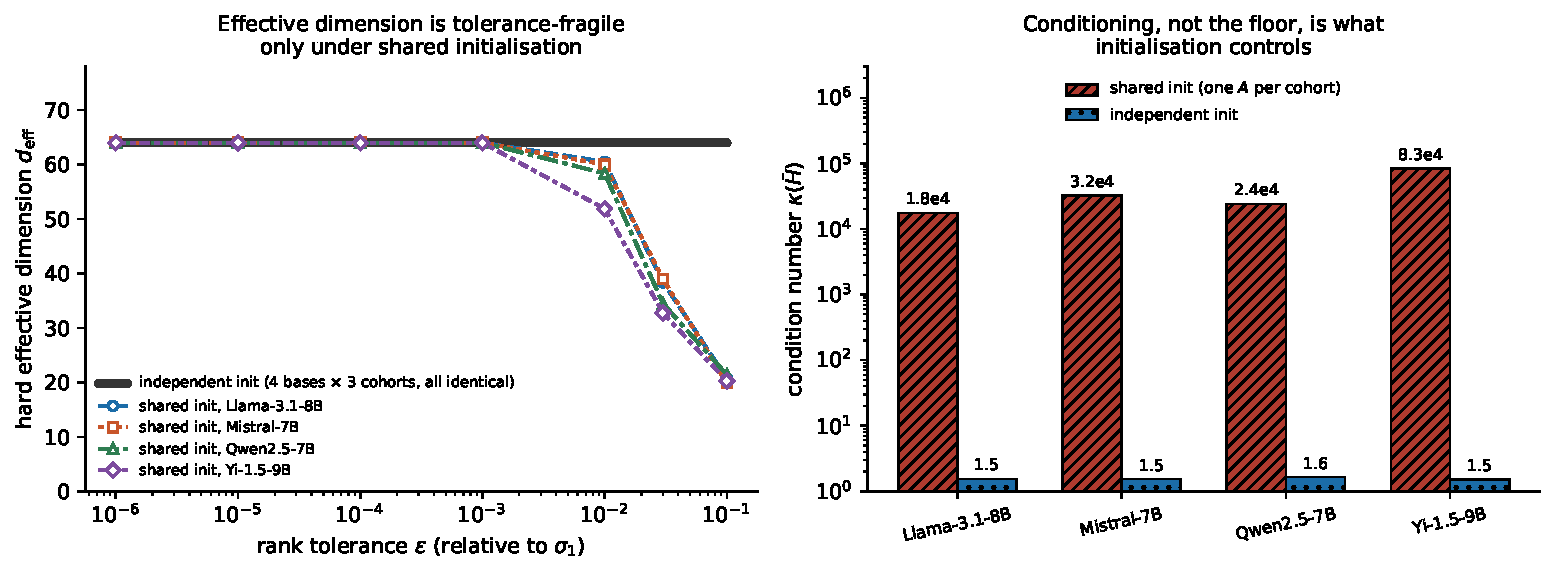
\includegraphics[width=\textwidth]{figures/figure_two_regimes.pdf}
\caption{The two regimes. \textbf{Left:} hard effective dimension against
rank tolerance. All twelve independently initialised cells hold
$\deff = Tr = 64$ at every tolerance across four decades; the shared cohorts
match only at numerically loose tolerances and fall to $\approx 20$ by
$\epsilon = 10^{-1}$. Since $\deff = Tr$ holds exactly in both, the
irreducible floor is zero in both (\S\ref{subsec:floor-zero}).
\textbf{Right:} what does separate them, the condition number of $\bar H$,
four to five orders of magnitude apart.}
\label{fig:two-regimes}
\end{figure}

Table~\ref{tab:conditioning} gives the result. The condition number of
$\bar H$ differs by four to five orders of magnitude between the two
conditions. The exact interpolator is $43$ to $64$ times larger than the mean
task delta under shared initialisation, against $3.96$ to $4.00$ under
independent initialisation. That value is $T$, the identity for exactly
orthogonal subspaces, and recomputing with the degenerate adapter dropped
returns $2.96$ to $3.00$ at $T=3$ (Appendix~\ref{app:t3}). Neither is
fitted. We record this as a correctness check on the
implementation and nothing more: reproducing an identity confirms the code
computes what we intend, and says nothing about whether the quantity
matters. \S\ref{subsec:ridge} is where that is tested.

So initialisation does not set the floor. It sets how ill-conditioned the
merge problem is, and therefore how large a solution must be to interpolate
the tasks.

\paragraph{Is $\kappa(\bar H)$ a property of the cohort or of our
surrogate?} $\bar H$ is built from the LoRA factors under the
specialisation $H_t = P_{V_t}$, so the question is fair and we answer it
only partly. What is surrogate-independent is the geometry: the principal
cosines and $\sigma_{\max}$ in Table~\ref{tab:geometry} are properties of
the row spaces $\range(A_t^\top)$ alone, and any $H_t$ with
$\range(H_t) = V_t$ inherits the near-degeneracy of $\sum_t P_{V_t}$,
because that degeneracy is the overlap of the $V_t$ and not a choice of
metric. What is \emph{not} surrogate-independent is the specific value of
$\kappa$, which would change under a Fisher-weighted $H_t$ with a spread
spectrum. We therefore read $\kappa(\bar H)$ as a calibrated index of
subspace overlap rather than as the condition number any particular solver
will encounter, and we have not measured the latter.

\paragraph{A mismatch of objects, and what closes it.} Three different
objects appear in the argument so far, and we flag that rather than let a
reader find it. Theorem~\ref{thm:general} constrains $w^\star \in \R^d$ with
no rank constraint. The interpolator $\tauH$ whose norm we report above has
rank up to $Tr = 64$. But our merge pipeline truncates every method back to
rank $r = 16$ for deployment parity, so the object whose norm we measure is
not one the pipeline can return, and the ridge sweep of
\S\ref{subsec:ridge} tests conditioning through a rank-$16$-constrained
solver.

That mismatch is testable, so we tested it: we repeated the
ridge sweep with the post-merge truncation disabled
(\S\ref{subsec:untruncated}), and it does survive: the unregularised
shared-versus-independent ratio is $25$ to $117$ times, against $2.1$ to
$65$ with truncation, on all four base models. Truncation was not producing
the effect. It was \emph{masking} part of it, which is what one should
expect, since discarding all but the leading $16$ directions of a rank-$64$
interpolator discards most of the ill-conditioned subspace along with them.

What remains open is only the first of the three objects. The theorem
constrains an unconstrained $w^\star$, and every merge we run is rank
constrained, so the bound bears on our measurements by analogy at that step
and not by derivation. That is a real limitation and it is not closed by
anything in this paper.

\subsection{The audit}
\label{subsec:audit}

Everything above is computed from the adapter weight matrices: no forward
passes, no evaluation data, no merging. It costs about one CPU minute for a
cohort of four rank-16 adapters. What it reports is not ``how much of your loss
is irreducible'', which is zero in every case we have seen, but where your
cohort sits on the conditioning axis of Table~\ref{tab:conditioning}, which
\S\ref{subsec:ridge} shows determines whether an unregularised solve-based
merge will work at all.

The whole of it is five lines, stated in full as
Algorithm~\ref{alg:audit}. Given $T$ adapters, for each of a sample of
layers, orthonormalise the rows of each adapter's $A$ factor and measure how
aligned the resulting subspaces are.

\begin{algorithm}[t]
\caption{The pre-merge conditioning audit. It reads only the $A$ factors of
the adapter files: no $B$ factors, no base weights, no forward passes and no
evaluation data, which is what makes it runnable before committing to a
merge.}
\label{alg:audit}
\begin{algorithmic}[1]
\Require Adapters $\{(A_t, B_t)\}_{t=1}^{T}$ trained on a common base; layer
  sample $\mathcal{L}$; thresholds $c_{\mathrm{hi}} = 0.9$,
  $c_{\mathrm{lo}} = 0.5$, registered in advance
  (\S\ref{subsec:prereg-docs}) and used unchanged
\Ensure Median principal-angle cosine $\bar c$, and a regime label
\State $C \gets \emptyset$
\For{each layer $\ell \in \mathcal{L}$}
  \For{$t = 1$ \textbf{to} $T$}
    \State $V_t \gets \mathrm{orth}\bigl(A_t^{(\ell)\top}\bigr)$
      \Comment{orthonormal basis of task $t$'s row space, $r$ columns}
  \EndFor
  \For{each pair $i < j$}
    \State $C \gets C \cup \operatorname{svals}\bigl(V_i^{\top} V_j\bigr)$
      \Comment{cosines of the principal angles}
  \EndFor
\EndFor
\State $\bar c \gets \operatorname{median}(C)$
  \Comment{median over pairs and over layers}
\If{$\bar c > c_{\mathrm{hi}}$}
  \State \Return $(\bar c,\ \textsc{collapsed})$
\ElsIf{$\bar c < c_{\mathrm{lo}}$}
  \State \Return $(\bar c,\ \textsc{separated})$
\Else
  \State \Return $(\bar c,\ \textsc{indeterminate})$
\EndIf
\end{algorithmic}
\end{algorithm}

\begin{center}
\fbox{\begin{minipage}{0.94\linewidth}
\textbf{How to read what Algorithm~\ref{alg:audit} returns:}
\begin{itemize}[leftmargin=*,itemsep=1pt,topsep=3pt]
  \item $\bar c > 0.9$ --- \textbf{collapsed}. Do not run an unregularised
        solve-based merge. Add a ridge, starting at $\lambda \approx 0.01$,
        or use a method that averages.
  \item $\bar c < 0.5$ --- \textbf{separated}. Conditioning is not your
        problem; the ridge buys between $0.00$ and $0.10$ nats.
  \item Between the two --- one of our $45$ public cohorts landed here and we
        have no advice for it.
\end{itemize}
\smallskip
Cost $O(T^{2} r^{2} d)$ per layer: about one CPU minute at $T = 4$, $r = 16$
over eight layers, with no forward passes and no evaluation data.
Implementation: \texttt{measure\_subspace\_geometry.py}.
\end{minipage}}
\end{center}

The $0.9$ and $0.5$ cutoffs are those registered before the public-cohort
audit of \S\ref{subsec:prevalence} and are used unchanged here. They are not
tuned, and on this evidence they do not need to be: the two populations differ
by more than an order of magnitude in $\bar c$, so any cutoff between them
gives the same partition, and $44$ of $45$ public cohorts fall outside the
interval entirely. \textbf{The $\lambda \approx 0.01$ is a starting point, not
a derived optimum.} \S\ref{subsec:ridge} finds $\lambda^\star = 0.01$ on seven
of eight arms, but also finds that how much regularisation is needed does not
track the conditioning, so a short sweep is worth more than our number.

\paragraph{Can I repair the adapters instead of the merge?} It is the first
thing a practitioner with a collapsed cohort and no budget to retrain will
think of, so it deserves an answer even though we did not test it. Orthogonalise
or re-randomise the $A$ factors, the thought goes, and the subspaces separate.

The trouble is that $A$ cannot be changed on its own. What the model computes
is $BA$, so replacing $A_t$ by $Q A_t$ for any invertible $Q$ leaves the
adapter's function unchanged only if $B_t$ becomes $B_t Q^{-1}$, and then the
product is identical and so is every quantity in this section: the row space
$\range(A_t^\top)$ is unchanged by an invertible map applied on the left, so
the principal cosines, $\bar H$ and its conditioning are all exactly what they
were. A repair that preserves each adapter's behaviour cannot change the
geometry, because the geometry is a property of that behaviour. A repair that
changes the geometry changes what each adapter does, and then the merge is
being asked to combine different models from the ones that were validated.

There is a narrow exception worth naming: the row spaces here have dimension
$r = 16$ inside $d = 4096$, and the near-collinearity is between spaces, not
within them, so one could project each $A_t$ onto a private slice of a
partition of the ambient space. That is a real construction and it is not free:
it discards the components of each task's update outside its assigned slice,
which is a lossy edit to a trained adapter, and whether the loss is tolerable
is exactly the question the merge was supposed to answer. We have not measured
it, we do not recommend it on the strength of an argument, and we flag it as
the natural next experiment for anyone who cannot retrain.

What we do recommend for a cohort that is already collapsed is the ridge, which
\S\ref{subsec:ridge} and \S\ref{subsec:downstream-cond} measure, costs one
hyperparameter, and leaves the adapters untouched.

\subsection{Scope: one adapter in four did not learn}
\label{subsec:scope}

On all four bases and in both conditions, the translation adapter fails to
beat the base model at its own task or is beaten there by another task's
adapter; the other three tasks train cleanly, improving $10$ to $70\%$ over
base with the specialist best on its own task in every cell
(Appendix~\ref{app:geometry}). Our cohorts are therefore $T=4$ nominal and
$3$ effective, and we describe them that way throughout.

\paragraph{We know why, and it is a data-pipeline defect rather than a
training failure.} Failing on four bases in both arms is too systematic to
be a bad run, so we diagnosed it, which needs no retraining. Translation is
the only task in the matrix configured to stream its training set, and the
streaming branch of our loader takes the first $n$ examples in corpus
order, while the branch every other task takes shuffles first. WMT19 de-en
is a concatenation of sub-corpora of roughly $35$M pairs, so an unshuffled
prefix of $7500$ samples whichever sub-corpus is written first rather than
the corpus. Measuring the prefix the trainer actually saw against a
shuffled sample of the same split and against the evaluation split settles
what happened: the prefix is parliamentary proceedings, at $17.4$
occurrences per $1000$ tokens of a small set of parliamentary terms against
$0.6$ in the shuffled control and $2.8$ in the news-domain evaluation
split, with a type-token ratio of $0.11$ against $0.30$ shuffled. The
adapter was trained on $7500$ consecutive sentences of one narrow register
and evaluated on another.

That is a defect in our configuration, not a property of translation as a
task or of LoRA. \textbf{We report it rather than repairing it}, because
repairing it means retraining the cohort and re-running every cell measured
on it, and the pre-registered comparisons in \S\ref{sec:methods} are all
paired \emph{within} a cohort: a cohort where one member is weak is a valid
cohort for asking whether initialisation geometry changes a merge, so long
as both arms contain the same weak member, which they do. What it is not is
a cohort of four well-trained adapters, and we make no claim about that
case.

Two further things bound the damage and one does not. Worst-task excess is never
driven by the degenerate adapter: across the $84$ independent-cohort cells the
argmax is \texttt{gsm8k} in $64\%$ and \texttt{alpaca} in $36\%$, and
translation never. And every geometry and conditioning quantity above is
reported at both $T=4$ and $T=3$ in Appendix~\ref{app:geometry}; the
shared-versus-independent contrast is unchanged to three decimals. What is
\emph{not} bounded is that the merged models contain an untrained member. That
is arguably realistic, since practitioners merge adapters of uneven quality,
but it is not the same experiment as four well-trained adapters, and we make
no claim about the latter.



\section{A First-Order Theory of the Collapse}\label{sec:drift-theory}
% Review item 6. Registered in notes/prereg_drift_theory_2026-09-23.md
% (ba51184) before any quantity below was computed; analyzer
% code/phase3/scripts/drift_theory.py (f632b12, fix 2d38d5a).

The measurements of \S\ref{subsec:conditioning} say that a shared
initialisation raises $\kappa(\bar H)$ by four orders of magnitude and the
norm of the exact interpolator by a factor of ten. This section derives both
from one assumption, that each adapter's $A$ factor is a small displacement of
a common start, and tests the derivation against the adapters. The result
explains the size of the effect, predicts how it scales with training, and
corrects a tempting shortcut.

\paragraph{Set-up.} In a shared-initialisation cohort, $A_t = A_0 + E_t$. Let
$W_0 \in \R^{d\times r}$ be an orthonormal basis of the row space of $A_0$ and
$P_\perp = I - W_0 W_0^\top$. Whenever $W_0^\top A_t^\top$ is invertible, the
row space $V_t$ of $A_t$ is exactly the graph of a \emph{tilt}
\begin{equation}\label{eq:tilt}
  X_t \;=\; P_\perp A_t^\top \bigl(W_0^\top A_t^\top\bigr)^{-1} \in \R^{d\times r},
  \qquad V_t = \operatorname{col}(W_0 + X_t),
\end{equation}
and the principal angles between $V_t$ and the starting subspace satisfy
$\tan\theta_i = \sigma_i(X_t)$. The tilt is of the order of the relative
displacement, $\|X_t\| \lesssim \|E_t\|/\sigma_{\min}(A_0)$.

\begin{proposition}[First-order conditioning of a shared cohort]
\label{prop:drift}
Let $Y = [X_1 - \bar X, \dots, X_T - \bar X] \in \R^{d\times Tr}$ collect the
centred tilts, $\Sigma_X = \tfrac1T Y Y^\top$, and write
$D_t = M_t (W_0 + X_t)^\top$ for the task updates in graph coordinates. To
leading order in the tilt,
\begin{enumerate}[leftmargin=*,itemsep=1pt,topsep=2pt]
\item $\bar H$ has $r$ eigenvalues $1 - O(\|X\|^2)$ and $(T-1)r$ eigenvalues
  equal to the nonzero eigenvalues of $\Sigma_X$, so
  $\kappa(\bar H) \approx 1/\lambda_{\min}^{+}(\Sigma_X)$;
\item the exact interpolator is $\tauH \approx a\,W_0^\top + b$ with
  $b = [M_1 - \bar M, \dots, M_T - \bar M]\, Y^{+}$ and $a = \bar M - b\bar X$;
\item under a uniform rescaling of the displacements $E_t \mapsto sE_t$,
  $\kappa(\bar H) \propto s^{-2}$ while
  $\|\tauH\|/\|\bar\Delta\| \propto s^{-1}$.
\end{enumerate}
\end{proposition}

The derivation (Appendix~\ref{app:drift-theory}) expands each projector to
second order in $X_t$ and takes the Schur complement of $\bar H$ on
$V_0^\perp$; the interpolation conditions $\tauH(W_0 + X_t) = M_t$ then
separate into a component along $W_0$ and one along the centred tilts.

\paragraph{Two consequences.} First, amplification is \emph{first} order in
the inverse displacement, not second. A rough argument gives
$\|\tauH\|/\|\bar\Delta\| \sim 1/\varepsilon^{2}$, which at the measured
$\varepsilon \approx 0.13$ is $59$, uncomfortably close to the measured $43$
to $64$. The proposition says that agreement is a coincidence: $\kappa$ is the
quantity that goes as $\varepsilon^{-2}$. Second, $\kappa(\bar H)$ is set by
the \emph{smallest} singular value of the displacement spread, not by its size.
Training moves each $A$ by about $13\%$, which on its own would give
$\kappa \sim 1/\varepsilon^2 \approx 60$; the measured $10^{4}$ to $10^{5}$
means the displacements are far from isotropic, with some directions of the
spread almost unexcited. This also suggests why the amount of regularisation
needed did not track $\kappa$ in \S\ref{subsec:ridge}: $\kappa$ is fixed by
the weakest direction, while what a ridge must suppress is the part of $b$
carried by the bulk of the spread. That reading was formed after the
$\lambda^\star$ values were known, so it is offered as a hypothesis; the
ridge rule of \S\ref{subsec:lambda-rule} is its prospective test.

\paragraph{Tests, registered before computation.} All five pre-registered
predictions hold (Table~\ref{tab:drift-theory}).
\emph{The formula}: on the drift cohort, whose $A_0$ was saved before the first
optimiser step, the first-order predictions of $\kappa(\bar H)$ and of the
amplification equal the exact values to three digits at $25$, $50$, $75$ and
$100\%$ of training (ratio $1.000$ throughout), and the reference-free
version, which needs no $A_0$ and takes the consensus subspace as $W_0$, does
the same on all twelve shared cohorts of the four bases.
\emph{The order}: scaling the measured displacements by
$s \in \{0.05, 0.1, 0.2, 0.5, 1\}$ gives exact log-log slopes of $-2.00$ for
$\kappa$ and $-1.01$ for the amplification, against the registered bands
$[-2.2, -1.8]$ and $[-1.2, -0.8]$; the rival $\varepsilon^{-2}$ form for the
amplification is excluded.
\emph{Across training}: both quantities fall monotonically as the adapters
drift, $\kappa$ from $2.7\times10^{4}$ to $1.1\times10^{4}$ and the
amplification from $61$ to $44$, the last inside the range
Table~\ref{tab:conditioning} reports for the final adapters of all four bases.

\begin{table}[t]
\centering
\small
\caption{The first-order theory against the exact quantities. Drift cohort
(Llama-3.1-8B, $A_0$ saved), median over eight layers. Ratios are
prediction / exact. The dial rescales the final displacements by $s$.}
\label{tab:drift-theory}
\begin{tabular}{lcccc}
\toprule
checkpoint & $\kappa(\bar H)$ & ratio & $\|\tauH\|/\|\bar\Delta\|$ & ratio \\
\midrule
$25\%$  & $2.67\times10^{4}$ & $1.000$ & $61.4$ & $1.000$ \\
$50\%$  & $1.57\times10^{4}$ & $1.000$ & $51.3$ & $1.000$ \\
$75\%$  & $1.17\times10^{4}$ & $1.000$ & $45.4$ & $1.000$ \\
$100\%$ & $1.09\times10^{4}$ & $1.000$ & $44.3$ & $1.000$ \\
\midrule
dial $s$ & \multicolumn{2}{c}{$\kappa(\bar H)$} & \multicolumn{2}{c}{$\|\tauH\|/\|\bar\Delta\|$} \\
\midrule
$0.05$ & \multicolumn{2}{c}{$4.34\times10^{6}$} & \multicolumn{2}{c}{$904.9$} \\
$0.1$  & \multicolumn{2}{c}{$1.09\times10^{6}$} & \multicolumn{2}{c}{$452.3$} \\
$0.2$  & \multicolumn{2}{c}{$2.72\times10^{5}$} & \multicolumn{2}{c}{$225.9$} \\
$0.5$  & \multicolumn{2}{c}{$4.35\times10^{4}$} & \multicolumn{2}{c}{$89.9$} \\
$1$    & \multicolumn{2}{c}{$1.09\times10^{4}$} & \multicolumn{2}{c}{$44.3$} \\
\midrule
log-log slope & \multicolumn{2}{c}{$-2.00$} & \multicolumn{2}{c}{$-1.01$} \\
\bottomrule
\end{tabular}
\end{table}

\subsection{Task count, rank and initialisation scheme}
\label{subsec:tr-sweep}

The proposition says the collapse is set by initialisation and its severity
by the spread of the displacements, so it should hold at any task count and
rank, with the conditioning worsening as more tilts crowd the same starting
subspace. We tested that on Llama-3.1-8B (registration
\texttt{prereg\_new\_cohorts}, Part R), training new adapters for four further
tasks (Dolly, XSum, CodeAlpaca, and English-to-French translation) and for
ranks $8$ and $64$, in both initialisation arms. All five registered
predictions hold (Table~\ref{tab:tr-sweep}). The regime is set by
initialisation at every size: shared cohorts sit at median cosine $0.990$ to
$0.999$ and independent ones at $0.032$ to $0.099$. The conditioning grows with
the task count, $\kappa(\bar H) = 3.9\times10^{3}$, $1.1\times10^{4}$ and
$3.9\times10^{4}$ at $T = 2, 4, 8$, and with the rank, $5.6\times10^{3}$,
$1.1\times10^{4}$ and $4.1\times10^{4}$ at $r = 8, 16, 64$. The first-order
formula matches the exact values on every shared configuration (ratio
$1.000$), and on the independent arm the amplification is the orthogonal value
$T$ ($1.99$, $4.00$, $7.91$). The solver consequence travels with it:
unregularised adapter-only RegMean is $2.5$ to $65$ times worse on the shared
arm at every configuration, while task arithmetic moves by at most $0.008$
nats.

\begin{table}[t]
\centering
\small
\caption{The collapse across task count and rank (Llama-3.1-8B). Median cosine,
$\kappa(\bar H)$ and amplification are exact; the ratio is the first-order
prediction over the exact $\kappa$. The last column is unregularised
adapter-only RegMean, shared over independent worst-task excess.}
\label{tab:tr-sweep}
\begin{tabular}{lcccccc}
\toprule
 & \multicolumn{2}{c}{median cosine} & \multicolumn{2}{c}{shared arm} &
 formula & RegMean \\
configuration & shared & indep. & $\kappa(\bar H)$ & amplification & ratio & shared/indep. \\
\midrule
$T=2$, $r=16$  & 0.996 & 0.045 & $3.9\times10^{3}$ & 17.9 & 1.000 & 33.5 \\
$T=4$, $r=16$  & 0.995 & 0.047 & $1.1\times10^{4}$ & 45.3 & 0.999 & 6.0 \\
$T=8$, $r=16$  & 0.996 & 0.047 & $3.9\times10^{4}$ & 90.4 & 1.001 & 2.5 \\
$T=4$, $r=8$   & 0.990 & 0.032 & $5.6\times10^{3}$ & 30.2 & 1.000 & 4.8 \\
$T=4$, $r=64$  & 0.999 & 0.099 & $4.1\times10^{4}$ & 84.7 & 0.999 & 65.0 \\
\bottomrule
\end{tabular}
\end{table}

\paragraph{An initialisation that collapses whatever the seed.} PiSSA sets $A$
from the principal singular vectors of the base weight, so the proposition
predicts a collapsed cohort even with independent seeds. Four PiSSA adapters
trained with the independent arm's seeds (Part P) are collapsed at median
cosine $0.999$, and their trained row spaces stay at principal cosine $0.9996$
of the base weight's top-$r$ right singular vectors: training displaces them
too little to leave the shared starting subspace. Both registered predictions
hold. A shared seed is therefore one route into the regime, not the only one.

\paragraph{What the proposition does not do.} It is a leading-order
expansion checked numerically, not a bound with explicit constants, and it
describes the shared regime only; in the independent regime the tilts are not
small and the amplification is $T$ by a separate identity
(\S\ref{subsec:conditioning}). It explains the conditioning the solvers see;
whether a given solver is exposed to it is the separate question of
\S\ref{sec:methods}.


\section{Which Merges the Collapse Reaches}\label{sec:methods}\label{sec:exposure}
% Restructured 2026-09-28 from method_tests.tex (verbatim move, then edited).
\subsection{Does the conditioning matter? Only for methods that solve}
\label{subsec:ridge}

\S\ref{subsec:conditioning} found a four-order-of-magnitude difference in
$\kappa(\bar H)$ between the two initialisation regimes. A difference that
size which nothing observable depends on would be a curiosity, so we tested
it, pre-registering the prediction before running the cells.

\paragraph{First, the null, and what it can actually detect.} We compare
every method on matched cohorts, same method, same base, shared against
independent initialisation, with three cohorts per arm so the
pre-registered gate can be applied: a cell counts as an effect only if the
mean difference exceeds $\max(0.005, 2\,\mathrm{SE})$. Across $20$
base-by-method cells, $15$ show no detectable effect, $5$ favour
independent initialisation, and none favours shared.

The number that matters alongside that is the smallest effect the design
could have found, because a null without one is not evidence of absence.
The gate sits at $0.0052$ nats in the median cell and $0.0109$ in the
worst, so the honest statement is \emph{no effect detectable at about
$0.01$ nats}, not \emph{no effect}. It also disposes of a smaller number
that has been quoted in this setting, a mean difference of $0.0014$ nats
against a metric resolution of about $0.001$: that difference sits below
the median gate, so it is a quantity this design cannot resolve in either
direction.

The five cells that do clear the gate are worth naming rather than
averaging away, because four of them are not spread at random. Three are
the subspace-alignment method, on Mistral, Qwen and Yi, at $0.0096$ to
$0.0129$ nats; the others are TIES on Llama at $0.0151$ and TVQ on Yi at
$0.0087$. Task arithmetic and DARE, the two methods closest to a plain
mean, show nothing anywhere. That ordering is the one the mechanism below
predicts: a method that explicitly operates on the subspace geometry is
the heuristic most exposed to a change in that geometry, and it gains from
the cohort whose subspaces are not near-collinear. The effect is small,
consistent in direction, and we do not build anything on it.

\paragraph{The same null in a unit we do not disclaim.} Everything above is
worst-task NLL excess, and \S\ref{sec:discussion} reports that this metric does
not track downstream accuracy across methods and on one benchmark ranks them
backwards. That objection lands harder on a null than on an effect: the
differences here are hundredths of a nat, which is the range in which we have
told the reader not to trust the metric. Meanwhile the positive result beside
it, the solver collapse, has two units. Reporting one half in a disputed unit
and the other half in two is an asymmetry we would rather remove than defend,
so we pre-registered the null in accuracy as well: first at one cohort per
arm, where no cell cleared a binomial gate of about $6$ points on GSM8K and
$11$ on HumanEval (Appendix~\ref{subsec:heur-n1}), and then, because a null at
that resolution is weak, as an equivalence test at three cohorts per arm
(\texttt{prereg\_heuristics\_tost}).

\begin{table}[t]
\centering
\small
\caption{The heuristics in downstream accuracy at three cohorts per arm, as an
equivalence test. $\bar d$ is the mean over the four bases of
$\mathrm{acc}_{\mathrm{indep}} - \mathrm{acc}_{\mathrm{shared}}$, so a negative
value favours the shared arm; the interval is the $90\%$ interval of the two
one-sided tests, and ``margin'' is the smallest equivalence margin the method
passes. The registered margins are $0.03$ on GSM8K and $0.05$ on HumanEval, and
every method passes both. GSM8K exact match at $n = 500$, HumanEval pass@1 at
$n = 164$; $240$ cells.}
\label{tab:heur-tost}
\begin{tabular}{lcccccc}
\toprule
 & \multicolumn{3}{c}{GSM8K} & \multicolumn{3}{c}{HumanEval} \\
method & $\bar d$ & $90\%$ interval & margin & $\bar d$ & $90\%$ interval & margin \\
\midrule
task arithmetic & $-0.003$ & $[-0.009, +0.003]$ & $0.009$ & $-0.019$ & $[-0.030, -0.008]$ & $0.030$ \\
TIES & $-0.013$ & $[-0.020, -0.006]$ & $0.020$ & $-0.007$ & $[-0.021, +0.007]$ & $0.021$ \\
DARE & $-0.007$ & $[-0.015, +0.000]$ & $0.015$ & $-0.016$ & $[-0.021, -0.010]$ & $0.021$ \\
TVQ$_2$ & $+0.004$ & $[-0.004, +0.012]$ & $0.012$ & $+0.004$ & $[-0.013, +0.021]$ & $0.021$ \\
repaired KnOTS & $-0.009$ & $[-0.015, -0.002]$ & $0.015$ & $-0.009$ & $[-0.022, +0.005]$ & $0.022$ \\
\bottomrule
\end{tabular}
\end{table}

\textbf{All five heuristics are equivalent across the two regimes} within the
registered margins, $3$ accuracy points on GSM8K and $5$ on HumanEval, and each
would pass at a margin of $0.9$ to $2.0$ points on GSM8K and $2.1$ to $3.0$ on
HumanEval (Table~\ref{tab:heur-tost}). One of the forty base-by-method cells
clears the per-cell gate: TIES on Llama at HumanEval, where the shared arm
scores $6.5$ points higher. It is the cell that came within $97\%$ of the gate
at one cohort per arm, in the same direction. Three of the four registered
predictions therefore hold, and from here on the null is stated as equivalence
rather than as the absence of a detected effect. It is a statement at these
margins: an effect of one or two points fits inside them.

The fourth prediction failed, and it concerns direction. At one cohort per arm,
$26$ of the $38$ non-zero differences had favoured the shared arm
($p = 0.034$); we had not registered that test, so we did not report the lean
as a finding. We registered the sign test for the three-cohort design and
predicted that the lean would not survive. It survives: $29$ of the $38$
non-zero per-base differences favour the shared arm, an exact sign test gives
$p = 0.0017$, and eight of the ten method-by-benchmark means are negative, TVQ
being the exception on both benchmarks. By the registered branch we report it
in its measured direction: \textbf{on these cohorts the averaging and
sparsifying heuristics score slightly higher when the adapters share their
initialisation}, by at most $1.9$ points on average, well inside the
equivalence margins. It runs opposite to the five NLL cells above, all of which
favoured independent initialisation, so the two units disagree about a
direction while agreeing that nothing is large. It is not the solver mechanism,
since no heuristic enters the ill-conditioned directions on either arm
(Table~\ref{tab:mechanism}), and we have no tested explanation for it. For
practice it means that someone merging with a heuristic loses nothing by a
shared initialisation, and may gain a point.

\paragraph{Then the mechanism, measured.} The explanation for the other
$15$ cells is that those methods never go near the ill-conditioned
direction. That is a measurement rather than an assertion, and it needs no
forward passes: every merge here is weight
arithmetic on the adapter factors. For each merged solution we report its
norm relative to the mean task delta, and the share of its energy lying in
the bottom quartile of $\bar H$'s eigen-directions, in the projected
coordinates of \S\ref{subsec:conditioning}.

\begin{table}[t]
\centering
\small
\caption{What each solution does with the ill-conditioned directions.
Amplification is $\|\Delta_{\mathrm{merged}}\|/\|\bar\Delta\|$; tail
fraction is the share of squared norm in the bottom quartile of $\bar H$'s
spectrum. Ranges are over the four base models. On the independent arm a
tail fraction near $0.21$ is what a generic direction gives when a quarter
of the dimensions holds a quarter of the energy, so the signature is the
$0.73$ to $0.80$ on the shared arm, not the baseline it is measured
against.}
\label{tab:mechanism}
\begin{tabular}{lcccc}
\toprule
 & \multicolumn{2}{c}{shared} & \multicolumn{2}{c}{independent} \\
solution & amplification & tail & amplification & tail \\
\midrule
mean task delta            & 1.00 & 0.000 & 1.00 & 0.21 \\
task arithmetic            & 0.99 & 0.000 & 0.86--0.92 & 0.20 \\
DARE                       & 0.98--0.99 & 0.000 & 0.86--0.90 & 0.20 \\
TIES                       & 1.98--2.04 & 0.000 & 2.04--2.22 & 0.21 \\
TVQ ($b{=}2$)              & 1.95--2.16 & 0.000 & 1.68--1.95 & 0.20 \\
\addlinespace
RegMean, minimal ridge     & 35.4--51.4 & 0.73--0.79 & 3.41--3.67 & 0.29 \\
our encoder, $\lambda = 0$ & 36.7--56.7 & 0.78--0.80 & 3.42--3.67 & 0.29 \\
our encoder, $\lambda^\star$ & 2.20--2.56 & 0.000 & 2.84--3.05 & 0.28 \\
\addlinespace
exact interpolator $\tauH$ & 43.4--64.1 & 0.62--0.66 & 3.96--4.00 & 0.28 \\
\bottomrule
\end{tabular}
\end{table}

Table~\ref{tab:mechanism} gives it. On the ill-conditioned cohort every
heuristic sits at one to two times the mean task delta with a tail
fraction that rounds to zero at three decimals, while both unregularised
solvers sit at $35$ to $57$ times with roughly three quarters of their
energy in the bottom quartile of the spectrum. They are the only methods
that go there, which is why they are the only methods the conditioning
reaches. One incidental check falls out: RegMean at minimal ridge and our
encoder at $\lambda = 0$ agree to two decimals on the independent arm
across all four bases, so two differently derived solvers land on the same
solution once the problem is well posed.

\paragraph{So we sweep the ridge, on two solvers.} To expose the
conditioning one needs a method that actually solves the system. Ours
does, and it carries a Tikhonov ridge, so sweeping $\lambda$ over seven
values, $0$, $0.01$, $0.03$, $0.05$, $0.13$, $0.30$ and $1.00$, on both
cohorts with rank pinned to $16$ in every cell isolates the effect.

\begin{table}[t]
\centering
\small
\caption{Worst-task NLL excess for the unregularised solve
($\lambda = 0$), and the gain from the best ridge. Conditioning is
invisible to the heuristics above and severe here.}
\label{tab:ridge}
\begin{tabular}{lccccc}
\toprule
base & \multicolumn{3}{c}{$\lambda = 0$} &
\multicolumn{2}{c}{ridge gain $L(0) - L(\lambda^\star)$} \\
 & shared & independent & ratio & shared & independent \\
\midrule
Llama-3.1-8B & 0.3081 & 0.0713 & $4.3\times$  & 0.2216 & 0.0000 \\
Mistral-7B   & 9.7799 & 0.1504 & $65\times$   & 9.7301 & 0.0952 \\
Qwen2.5-7B   & 0.1973 & 0.0256 & $7.7\times$  & 0.1867 & 0.0114 \\
Yi-1.5-9B    & 0.2490 & 0.1209 & $2.1\times$  & 0.2211 & 0.0904 \\
\bottomrule
\end{tabular}
\end{table}

Table~\ref{tab:ridge} gives the result. Unregularised, the same merge is
$2.1$ to $65$ times worse on the ill-conditioned cohort; on Mistral it
collapses outright to $9.78$ nats against $0.15$. The ridge gain is larger
on the shared arm on all four bases, which was the pre-registered
prediction and held.

The other half of the prediction failed. We also predicted that $\lambda^\star$ itself would be at least ten times
larger on the shared arm. It is not: $\lambda^\star$ is \emph{identical}
across arms on Mistral, Qwen and Yi ($0.13$, $0.13$, $0.30$), separating
only on Llama. How much regularisation is needed does not track
conditioning in any simple way; how much it buys does. By the
pre-registered rules this makes the test \textsc{partial}, and we claim
only the half that held.

\subsection{Both arms at three cohorts}
\label{subsec:shared-arm}

Table~\ref{tab:ridge} rests on one shared cohort against three independent
ones, so its noise gate borrowed its standard error entirely from the
independent side. A shared-versus-independent contrast measured that way is
three draws against one, and a reader is right to discount it. We registered
the completion in advance and ran the sweep on two further shared cohorts, so
both arms are $n = 3$ and the gate carries a term from each. This is a
replication of a result we had already published, so it could only cost us
something; the registration says so and fixes the consequence text for the
outcome where it fails.

It does not fail. With
$\mathrm{SE} = \sqrt{\mathrm{SE}_s^2 + \mathrm{SE}_i^2}$ and the gate at
$\max(0.005, 2\,\mathrm{SE})$, the ridge gain is larger on the shared arm on
\textbf{four of four} bases and the unregularised excess is worse there by at
least a factor of two on \textbf{four of four}: ratios of $4.42$, $76.2$,
$10.8$ and $2.82$, against gates of $0.024$, $4.26$, $0.128$ and $0.166$.
Mistral's shared arm averages $11.72$ nats at $\lambda = 0$ against $0.154$
independent.

One quantity is worth reporting because it could have embarrassed the earlier
table and does not. The published single-cohort value, \texttt{seed1}, sits
$0.23$, $0.53$, $0.75$ and $0.66$ standard deviations from its own arm's
three-cohort mean. We registered that a distance above $2$ on two or more
bases would oblige us to say the published value was unrepresentative of its
own arm. It is representative, and Table~\ref{tab:ridge}'s numbers stand as
single-cohort estimates of quantities the three-cohort means confirm.

\subsection{A second adapter-built solver: RegMean without data}
\label{subsec:regmean}

Everything above concerns one solver, and we built it. The first question a
referee asks is whether the effect belongs to the family or to our
implementation. RegMean~\citep{jin2023regmean} solves a least-squares system in
per-task input-activation Grams; its \emph{data-free, adapter-only} form, which
replaces each activation Gram by $A_t^\top A_t$, is a second solver whose
matrix is built from the adapters' own factors. We say plainly that this form
is a variant we constructed, not the published method, and it is exactly the
kind of solver the mechanism says is exposed; \S\ref{subsec:data-solvers}
tests the published method with real activation Grams, and two further
methods we did not build.

We swept it on the same grid and cohorts, registering two predictions: the
ridge gain larger on the shared arm, and the minimally regularised excess worse
there by at least a factor of two, each on at least three of four bases. The
numbers below use the Gram the method is defined with; an earlier version of
this table was computed with a fallback Gram by mistake, and
Appendix~\ref{subsec:gram-error} gives the account and both sets of numbers.

RegMean ships a regulariser of its own, and it is \emph{not} the Tikhonov
ridge swept here: it scales the non-diagonal entries of each Gram by
$\alpha$, default $0.9$. The $\lambda I$ in this table is ours, and
\S\ref{subsec:regmean-default} evaluates RegMean's own default end to end.

\begin{table}[t]
\centering
\small
\caption{Adapter-only RegMean on both cohorts, with the described Gram
$\sum_t A_t^\top A_t$. The minimally regularised reference is
$\lambda = 10^{-6}$ rather than $0$: the Gram has rank at most $Tr = 64$ in
$d = 4096$ dimensions, so $\lambda = 0$ is singular rather than
ill-conditioned. Our encoder solves inside $\range(\bar H)$, so its
$\lambda = 0$ is defined; each method is compared only against itself across
arms.}
\label{tab:regmean}
\begin{tabular}{llcccc}
\toprule
base & cohort & $\lambda = 10^{-6}$ & $\lambda^\star$ & gain & ratio \\
\midrule
Llama-3.1-8B & shared      & 0.2918 & 0.03 & 0.1781 & \multirow{2}{*}{$4.1\times$} \\
             & independent & 0.0710 & $10^{-6}$ & 0.0000 & \\
\addlinespace
Mistral-7B   & shared      & 10.1651 & 0.05 & 10.1155 & \multirow{2}{*}{$65.6\times$} \\
             & independent & 0.1551 & 0.05 & 0.1006 & \\
\addlinespace
Qwen2.5-7B   & shared      & 0.1504 & 0.05 & 0.1391 & \multirow{2}{*}{$5.8\times$} \\
             & independent & 0.0258 & 0.13 & 0.0117 & \\
\addlinespace
Yi-1.5-9B    & shared      & 0.2179 & 0.13 & 0.1947 & \multirow{2}{*}{$1.8\times$} \\
             & independent & 0.1206 & 0.13 & 0.0879 & \\
\bottomrule
\end{tabular}
\end{table}

Both predictions hold: the ridge gain is larger on the shared arm on four of
four bases, and the unregularised excess is at least twice as large there on
three of four (Yi reaches $1.8$). The effect is not a property of our encoder.

Two details are worth reporting. The selected ridge is the same on both arms
of Mistral and of Yi, so on this solver too the amount of regularisation
needed does not track the conditioning even though the amount it buys does,
the split our own sweep found. And Llama's independent arm selects the minimal
$\lambda$ and gains exactly zero: on a well-conditioned cohort there is nothing
to repair.

\subsection{Solvers built from data, whitening, and a diagonal}
\label{subsec:data-solvers}

The mechanism makes a sharper prediction than ``solvers are exposed''. The
collapse makes the matrix $\sum_t A_t^\top A_t$ ill-conditioned; a solver is
exposed if it inverts a matrix built from the adapters' own factors, and should
not be if its matrix comes from data or is diagonal, since a diagonal cannot see
overlap between subspaces. We registered that prediction for four published
methods, none of ours, before running any of them
(\texttt{prereg\_regmean\_real}, \texttt{prereg\_third\_solver}): RegMean with
real input-activation Grams at its published $\alpha = 0.9$; MaTS~\citep{tam2024mats}
with its blockwise (KFAC) Fisher solved by 100 conjugate-gradient iterations,
as in the official code; TSV-M~\citep{gargiulo2025tsv}, which whitens the
stacked singular vectors of the task updates and was therefore predicted to be
exposed; and diagonal Fisher merging~\citep{matena2022fisher}. Each ran on all
three cohorts of both arms on all four bases.

\begin{table}[t]
\centering
\small
\caption{Methods we did not build. Worst-task NLL excess, shared over
independent (mean over three cohorts per arm), and whether the difference
clears the registered gate $\max(0.005, 2\,\mathrm{SE})$. The prediction column
is the mechanism's, registered before any cell ran.}
\label{tab:data-solvers}
\begin{tabular}{llcccc}
\toprule
method & predicted & Llama & Mistral & Qwen & Yi \\
\midrule
RegMean, activation Grams & immune & $1.03$ & $1.14$ & $0.99$ & $1.13$ \\
MaTS (KFAC Fisher, CG)    & immune & $0.98$ & $0.94$ & $0.93$ & $0.99$ \\
diagonal Fisher           & immune & $1.08^{\ast}$ & $1.02$ & $0.96$ & $0.98$ \\
TSV-M (whitening)         & exposed & $1.08$ & $1.19^{\ast}$ & $0.81$ & $0.91^{\ast}$ \\
\bottomrule
\multicolumn{6}{l}{\footnotesize $^{\ast}$ clears the gate; for Yi the
difference favours the shared arm.}
\end{tabular}
\end{table}

The three immunity predictions hold (Table~\ref{tab:data-solvers}): RegMean
with activation Grams shows no effect on any base, in NLL or in accuracy
(Table~\ref{tab:regmean-acc}), MaTS none, and the diagonal
Fisher merge one small effect on Llama ($1.08$ times), below the registered
bound. The exposure prediction for TSV-M fails: it shows an effect on Mistral
only ($1.19$ times), the opposite sign on Yi, and nothing on Llama and Qwen, and
in accuracy no cell clears the gate on either benchmark. By the registered
branch, the whitening case was predicted and did not hold, and the exposure
rule is stated for solvers alone.

One registered detail also failed. We predicted that RegMean with activation
Grams would keep the pre-truncation norm of its solution within three times the
mean task delta; it reaches $2.2$ to $6.5$. The amplification is the same on
both arms (for example $3.15$ shared against $3.44$ independent on Llama),
because it comes from the activation Grams themselves, whose condition numbers
reach $10^{4}$ to $10^{7}$ whatever the initialisation. The immunity to
initialisation holds; the bound we put on the norm was wrong.

\paragraph{The rule this licenses.} Across eleven methods, nine of them not ours,
the collapse reaches exactly the merges that solve a linear system in a matrix
built from the adapters' own factors: our encoder and adapter-only RegMean.
It does not reach averaging or sparsifying heuristics, which are equivalent
across regimes within a few accuracy points (\S\ref{subsec:ridge}),
solvers whose matrix comes from data, a diagonal solver, or whitening.

\subsection{Does RegMean's published default already fix this?}
\label{subsec:regmean-default}

Our practical recommendation reduces to regularising a solve-based merge, and
RegMean ships a regulariser. If its default were already strong enough on a
collapsed cohort, the recommendation would shrink to the much smaller claim
that the audit tells you when the default matters. The question is worth
answering rather than leaving for a referee, and it is a lookup plus a
CPU-only computation.

RegMean's published regulariser scales the non-diagonal entries of each Gram
by $\alpha$, default $0.9$, which is equivalent to adding
$(1-\alpha)\operatorname{diag}(G)$: a shrinkage whose size the data sets,
rather than a free parameter. It does regularise, and on a rank-deficient Gram
it does make the system solvable. The question is whether it is enough.

On the shared-initialisation cohorts it is not, by about an order of
magnitude. Averaged over sampled layers, $\alpha = 0.9$ is equivalent to an
isotropic ridge of $5.2\times10^{-4}$ to $6.1\times10^{-4}$ across the four
bases, against the $\lambda^\star$ of $0.03$ to $0.13$ that the sweep selects on
the shared arm (Table~\ref{tab:regmean}): $50$ to $250$ times smaller. The
conditioning it leaves behind reflects that. The $\alpha$-shrunk system has condition number $6.6\times10^{3}$ to
$9.1\times10^{3}$, while $\lambda = 0.01$ brings the same layers to about
$1.5\times10^{2}$, a factor of $55$ apart. The default is on the wrong side of
the gap this paper is about.

The independent arm is the control, and it behaves as the story requires. The
\emph{same} default leaves $\kappa$ at $1.2\times10^{3}$ to $1.4\times10^{3}$
there, six to seven times lower than on the shared arm, while the equivalent
ridge it applies is identical to three significant figures
($5.2$ to $6.1\times10^{-4}$ on both arms). That is the point in one line:
$\alpha$-shrinkage is a fixed dose set by the data's scale and not by the
cohort's conditioning, so it neither knows nor cares which regime it is in.
On a well-conditioned cohort the dose is ample. On a collapsed one it is
far too small, and nothing in the method notices.

\paragraph{End to end.} The conditioning argument was a computation, so we
registered the merge itself (\texttt{prereg\_regmean\_real}): adapter-only
RegMean with $\alpha = 0.9$ and no ridge, on all three cohorts of both arms, in
NLL and in downstream accuracy. In NLL both registered predictions hold on three
of four bases. The shipped default is worse on the shared arm by $18$, $68$ and
$5.3$ times on Llama, Mistral and Yi, each past the gate; on Qwen it is $41$
times worse on average but one of the three shared cohorts sits far from the
other two ($2.54$ nats against $0.20$ and $0.22$), which widens the gate beyond
the difference. The audit's starting ridge, $\lambda = 0.01$, improves on the
default on the shared arm past the gate on the same three bases.

\begin{table}[t]
\centering
\small
\caption{RegMean end to end in downstream accuracy, mean over three cohorts per
arm. The first two column pairs are the adapter-only form (Gram
$\sum_t A_t^\top A_t$) at the shipped $\alpha = 0.9$ and at the audit's starting
ridge $\lambda = 0.01$; the last is the published method with activation Grams
at $\alpha = 0.9$. GSM8K exact match at $n = 500$, HumanEval pass@1 at
$n = 164$; $144$ cells.}
\label{tab:regmean-acc}
\begin{tabular}{llcccccc}
\toprule
 & & \multicolumn{2}{c}{adapter-only, $\alpha{=}0.9$}
   & \multicolumn{2}{c}{adapter-only, $\lambda{=}0.01$}
   & \multicolumn{2}{c}{activation Grams} \\
base & benchmark & shared & indep. & shared & indep. & shared & indep. \\
\midrule
Llama-3.1-8B & GSM8K     & 0.168 & 0.705 & 0.477 & 0.730 & 0.784 & 0.792 \\
             & HumanEval & 0.187 & 0.541 & 0.425 & 0.553 & 0.646 & 0.659 \\
Mistral-7B   & GSM8K     & \textbf{0.000} & 0.285 & 0.029 & 0.323 & 0.532 & 0.519 \\
             & HumanEval & \textbf{0.000} & 0.057 & 0.002 & 0.093 & 0.360 & 0.366 \\
Qwen2.5-7B   & GSM8K     & 0.148 & 0.611 & 0.580 & 0.625 & 0.624 & 0.617 \\
             & HumanEval & 0.510 & 0.683 & 0.589 & 0.685 & 0.726 & 0.728 \\
Yi-1.5-9B    & GSM8K     & 0.093 & 0.724 & 0.628 & 0.726 & 0.773 & 0.775 \\
             & HumanEval & 0.077 & 0.130 & 0.154 & 0.130 & 0.354 & 0.348 \\
\bottomrule
\end{tabular}
\end{table}

In accuracy the picture is sharper (Table~\ref{tab:regmean-acc}). On the shared
arm the shipped default loses most of GSM8K on every base, scoring $0.09$ to
$0.17$ where the same method reaches $0.61$ to $0.72$ on the independent arm,
and on Mistral it scores \textbf{zero on both benchmarks in all three shared
cohorts}. The starting ridge beats the default on the shared arm past the gate
on three of four bases on GSM8K (by $31$, $43$ and $54$ points on Llama, Qwen
and Yi) and on two on HumanEval (Llama and Qwen), so the registered accuracy
prediction holds. Mistral is the exception and we name it: $\lambda = 0.01$
does not rescue it ($0.029$ and $0.002$), and Table~\ref{tab:regmean} selects
$\lambda^\star = 0.05$ for this solver on that base, so the starting ridge is
where a sweep begins rather than an answer. The published method with
activation Grams, the control, scores the same on both arms in all eight
base-by-benchmark cells, within $1.3$ points everywhere, and is the strongest
merge in the table on every base: a practitioner who has the data RegMean was
designed for is unaffected by the collapse.

$\alpha$ is a documented knob, and a practitioner who lowers it is doing what
\S\ref{subsec:ridge} recommends. The claim is only that the shipped default does
not do it for them, and that nothing in the method signals when it should.

\subsection{The same test without rank truncation}
\label{subsec:untruncated}

\S\ref{subsec:conditioning} notes that our pipeline truncates every merge
back to rank $r$, so the sweep above tests conditioning through a
rank-constrained solver while the interpolator whose norm we report has
rank up to $Tr$. Repeating the sweep with truncation disabled removes that
mismatch, and the truncated sweep is then the comparison arm rather than
being re-run.

\begin{table}[htb]
\centering
\small
\caption{The conditioning link with rank truncation disabled. Worst-task NLL
excess in nats at $\lambda = 0$, and the shared-to-independent ratio with and
without truncation. The truncated column is the sweep of
Table~\ref{tab:ridge}, reproduced here as the comparison arm rather than
re-run. \textbf{Two entries here invite a second look and we have taken it.}
Mistral's shared value, $11.6283$, sits exactly $1.0000$ above RegMean's
$10.6283$ in Table~\ref{tab:regmean} at four decimals; the underlying numbers
are $11.628281$ and $10.628309$, so the gap is $0.999973$ and the agreement is
a coincidence between two different methods on two different runs rather than
a transcription. And Qwen's independent value matches
Table~\ref{tab:ridge}'s to four decimals, $0.025571$ against $0.025638$;
that one is not coincidence but the point of the table, since on a
well-conditioned cohort there is almost nothing in the discarded directions
for truncation to remove.}
\label{tab:untruncated}
\begin{tabular}{lcccc}
\toprule
 & \multicolumn{2}{c}{$\lambda = 0$ excess} & \multicolumn{2}{c}{shared / independent} \\
base & shared & independent & untruncated & truncated \\
\midrule
Llama-3.1-8B & 7.4266  & 0.0635 & $116.9\times$ & $4.3\times$ \\
Mistral-7B   & 11.6283 & 0.1582 & $73.5\times$  & $65\times$ \\
Qwen2.5-7B   & 0.8993  & 0.0256 & $35.2\times$  & $7.7\times$ \\
Yi-1.5-9B    & 3.1294  & 0.1227 & $25.5\times$  & $2.1\times$ \\
\bottomrule
\end{tabular}
\end{table}

Table~\ref{tab:untruncated} shows the link surviving on all four bases, with the effect \emph{larger}
without truncation, by factors of $25$ to $117$ against $2.1$ to $65$.
Truncation was not manufacturing the result; it was hiding part of it,
which is what one should expect when all but the leading $16$ directions
of a rank-$64$ interpolator are discarded and the ill-conditioned subspace
goes with them. The numbers we report as primary are therefore the
conservative ones.

\paragraph{What this licenses, and what it does not.} It licenses a
conditional recommendation: if you merge with a method that solves a
linear system, check your cohort's conditioning and regularise, because
unregularised it can fail by a factor of $65$ at rank $16$ and $117$
without truncation, on two solvers, one of which we did not build. It does
\emph{not} license the general advice to initialise independently. On the
methods most practitioners actually use the null above stands, in NLL and
as equivalence in accuracy, with two small qualifications that point in
opposite directions: in NLL the subspace-alignment method gains a little
from independent initialisation on three of four bases, and in accuracy
the heuristics as a group lean slightly toward the shared arm. We do not
dress either up as anything more.

\subsection{The collapse is visible in downstream accuracy}
\label{subsec:downstream-cond}

Everything above is measured in worst-task NLL excess, and
\S\ref{sec:discussion} reports that this metric does not predict downstream
accuracy across merge methods, and on HumanEval predicts it backwards. A
reader is entitled to extend that objection to the whole paper: if the metric
does not track model quality, why should any of these numbers matter?

The objection is about differences of hundredths of a nat between methods. The
conditioning effect is not that. At $\lambda = 0$ the shared-versus-independent
gap runs from $0.22$ to $11.56$ nats across the four bases at $n = 3$ per
arm ($0.13$ to $9.63$ from the single-cohort Table~\ref{tab:ridge}, which is
the same quantity measured with one draw), one to three orders of magnitude above
both the metric's resolution and the differences the correlation was computed
over. An effect that size either shows up in accuracy or the metric is
measuring something other than model quality. We registered the test without
knowing which, and fixed in advance that a null would move this limitation into
\S\ref{sec:intro} and delete the practice recommendations rather than defend
them.

\begin{table}[t]
\centering
\small
\caption{Downstream accuracy of the same merges, with the repaired scorers.
GSM8K exact match at $n = 500$, HumanEval pass@1 at $n = 164$, its whole test
split. Gate is $\max(5\text{ points}, 2\,\mathrm{SE})$ on the binomial. No cell
had a scorer discard: every generation was scored.}
\label{tab:downstream-cond}
\begin{tabular}{lcccccc}
\toprule
& \multicolumn{3}{c}{shared} & \multicolumn{3}{c}{independent} \\
base & $\lambda{=}0$ & $\lambda^\star$ & gain
     & $\lambda{=}0$ & $\lambda^\star$ & gain \\
\midrule
\multicolumn{7}{l}{\emph{GSM8K, exact match}} \\
Llama-3.1-8B & 0.318 & 0.654 & $+0.336$ & 0.708 & 0.712 & $+0.004$ \\
Mistral-7B   & \textbf{0.000} & 0.462 & $+0.462$ & 0.276 & 0.424 & $+0.148$ \\
Qwen2.5-7B   & 0.496 & 0.808 & $+0.312$ & 0.786 & 0.786 & $+0.000$ \\
Yi-1.5-9B    & 0.346 & 0.802 & $+0.456$ & 0.698 & 0.794 & $+0.096$ \\
\addlinespace
\multicolumn{7}{l}{\emph{HumanEval, pass@1}} \\
Llama-3.1-8B & 0.250 & 0.573 & $+0.323$ & 0.518 & 0.530 & $+0.012$ \\
Mistral-7B   & \textbf{0.000} & 0.244 & $+0.244$ & 0.067 & 0.189 & $+0.122$ \\
Qwen2.5-7B   & 0.530 & 0.744 & $+0.213$ & 0.726 & 0.738 & $+0.012$ \\
Yi-1.5-9B    & 0.024 & 0.091 & $+0.067$ & 0.049 & 0.067 & $+0.018$ \\
\bottomrule
\end{tabular}
\end{table}

\paragraph{It shows up, on both benchmarks.} The ridge improves the shared arm
past the gate on \textbf{four of four} bases on both benchmarks. The
difference-in-differences, which is the claim that the ridge helps
\emph{because of} conditioning rather than helping everything everywhere,
clears the gate on four of four on GSM8K and three of four on HumanEval; the
exception is Yi, where both arms sit near the floor of a benchmark it barely
solves at all ($0.024$ to $0.091$). By the registered rule, requiring either
prediction on at least three of four bases on at least one benchmark, the
outcome is \textsc{confirmed}.

\paragraph{The number worth stating plainly.} On Mistral, the shared-cohort
unregularised merge scores \textbf{zero} on both benchmarks. It is not
producing malformed output that a scorer discards: all $500$ GSM8K generations
and all $164$ HumanEval generations are non-empty, and none contains an
extractable answer or passes a test. The model generates fluent text and has
lost the capability entirely. One Tikhonov term on the same adapters recovers
$0.462$ and $0.244$. That is what four orders of magnitude of conditioning buys
in a unit a practitioner cares about.

\paragraph{What this does not license.} It does not show that worst-task NLL
excess predicts accuracy in general, and we do not claim it. The correlation
that fails in \S\ref{sec:discussion} is across merge \emph{methods} at fixed
cohort, and nothing here tests that. What it shows is that the specific effect
this paper is about is not an artifact of the metric, which is the objection it
was registered to answer.


\subsection{The same results with a working translation adapter}
\label{subsec:translation-fix}

Every cohort above contains a translation adapter that did not learn its task
(\S\ref{subsec:scope}). We retrained it with the one-line loader fix, a
shuffled stream, on Llama-3.1-8B and Mistral-7B in the shared and first
independent cohorts, with each cohort's own seeds, and re-ran the core cells on
the resulting cohorts (\texttt{prereg\_new\_cohorts}, Part T).

The fix helps but does not pass its registered test. The retrained adapter now
improves on the base model's translation loss (by $12\%$ on Llama, where the
original was $1.6\%$ worse, and by $6\%$ on Mistral), but another adapter in the
cohort is still better on translation, so by the registered criterion it has
not learned its task and the caveat of \S\ref{subsec:scope} stands as written.

On these cohorts every other registered prediction holds. The regimes are
unchanged (median cosine $0.995$ and $0.994$ shared, $0.047$ independent);
unregularised adapter-only RegMean is $6.0$ and $64.6$ times worse on the shared
arm with the larger ridge gain there; the five heuristics move by less than
$0.02$ nats in all ten cells; and in accuracy the encoder's $\lambda^\star$
recovers the shared arm past the gate on both bases and both benchmarks. On
Mistral the unregularised shared merge again scores $0.000$ on GSM8K and on
HumanEval, and the ridge again recovers $0.468$ and $0.244$. The results of this
section therefore do not depend on the adapter that failed to train, although
the cohort is still not four well-trained adapters.

\subsection{Setting the ridge}
\label{subsec:lambda-rule}

The practical advice is to regularise an adapter-built solve on a collapsed
cohort. How much is the natural next question, and the first-order theory
suggests a data-free answer: cap the condition number of the adapter Gram. We
registered such a rule before evaluating it anywhere
(\texttt{prereg\_lambda\_rule}): per layer, the smallest isotropic ridge that
brings the condition number of $\sum_t A_t^\top A_t$ on its range down to
$k = 100$, a round number fixed in advance, evaluated only on cohorts that no
ridge had been selected on.

The rule fails its main test. On all six collapsed cohorts of
\S\ref{subsec:translation-fix} and \S\ref{subsec:tr-sweep} it is worse than the
fixed $\lambda = 0.01$ (by $0.08$ to $4.2$ nats), although it beats RegMean's
shipped default on five of six. On the separated cohorts it is within $0.005$
nats of the unregularised solve on four of six; in the other two it is better by
more than that, which the registered test also counts as a miss. By the
registered branch, the recommendation stays as it was: on a collapsed cohort,
start near $\lambda = 0.01$ for adapter-only RegMean and sweep, since the
selected ridge varies by base (Table~\ref{tab:regmean}) and does not track the
conditioning. A data-free rule that sets the ridge well remains open.


\section{The Collapsed Regime in Public Adapters}\label{sec:public}
% Restructured 2026-09-28 from regimes.tex (verbatim move, then edited).
\subsection{The collapsed regime occurs in public adapters}
\label{subsec:prevalence}

Every cohort measured so far is one we trained ourselves, in both conditions,
deliberately. That is a controlled experiment and it establishes nothing about
anyone else's adapters. So we ran the audit of \S\ref{subsec:audit} over public
LoRA cohorts, under a protocol registered before any adapter was downloaded
(\S\ref{subsec:prereg-docs}). The registration exists because the failure mode
here is selection: an author who picks which cohorts to measure can produce any
prevalence they like.

\paragraph{Sampling frame, fixed in advance.} We walk the HuggingFace model
index filtered to \texttt{library\_name=peft}, sorted by downloads descending,
and group adapters into cohorts by (publisher, base model). Sorting by
downloads rather than recency or search relevance is a choice made in advance
and stated: it weights the sample towards adapters people actually use. A
cohort enters if it has at least two adapters on one base model, each a
readable PEFT LoRA of rank $\geq 4$ sharing at least one target module. Every
criterion is checkable from metadata before any weight is fetched, and
\textbf{no cohort was skipped after inspection}. We walked $1000$ models and
stopped at the registered target of $50$ cohorts; $330$ candidates were
rejected as cohorts of one and $282$ for having no readable adapter
configuration. Five of the $50$ could not be scored, leaving $45$.

\paragraph{Result.} Seventeen of the $45$ cohorts, \textbf{$37.8\%$}, have a
median principal cosine above $0.9$: the collapsed regime, in adapters we did
not train and did not select. The registered prediction was $20\%$.

\begin{table}[tb]
\centering
\small
\caption{Public LoRA cohorts under the audit of \S\ref{subsec:audit}. The
sampling frame and the $0.9$ threshold were registered before any adapter was
downloaded. The two populations are separated by more than an order of
magnitude in median principal cosine and do not overlap: only one cohort of
$45$ falls between $0.5$ and $0.9$.}
\label{tab:prevalence}
\begin{tabular}{lccc}
\toprule
 & cohorts & median principal cosine & $\|A_i - A_j\|_F/\|A_i\|_F$ \\
\midrule
collapsed, $\cos > 0.9$      & 17 & 0.915 -- 1.000 (med. 0.996) & 0.017 -- 0.760 \\
intermediate, $[0.5, 0.9]$   & 1  & 0.868 & --- \\
separated, $\cos < 0.5$      & 27 & 0.049 -- 0.440 (med. 0.076) & med. 1.414 \\
\bottomrule
\end{tabular}
\end{table}

\paragraph{The distribution is bimodal, and one number checks the
measurement.} Table~\ref{tab:prevalence} is not a continuum with a threshold
drawn through it. Forty-four of $45$ cohorts sit at one extreme or the other,
and the gap between the populations is wider than the spread within either.

The second column is an unplanned validation. If two adapters draw $A$
independently and $A$ moves little in training, then
$\|A_i - A_j\|_F^2 \approx \|A_i\|_F^2 + \|A_j\|_F^2$, so the ratio should be
$\sqrt 2 \approx 1.414$. The separated cohorts return a median of exactly
$1.414$. The collapsed cohorts run from $0.017$, adapters whose $A$ factors
agree to within $1.7\%$, up to $0.760$. We did not design this as a check and
it is not part of any registered rule, but it is the strongest evidence we have
that the audit measures what we claim: the separated population behaves
numerically like independent draws, because that is what it is.

\paragraph{What this does and does not establish.} It establishes that the
regime is common in released adapters, at a rate we can state with a frame a
reader can rerun. It does not by itself establish a consequence, which
\S\ref{subsec:public-merge} tests, or that published merging benchmarks are
affected, which Part B addresses (\S\ref{subsec:part-b}). Two of the $45$ have
members at differing LoRA rank, so their
$\|A_i - A_j\|_F$ comparison is undefined and only their cosine is reported;
both are separated. The audit's cost is unchanged from
\S\ref{subsec:audit}: about one CPU minute per cohort, and the entire sweep of
$45$ cohorts needed no GPU.

\paragraph{The three registered parts.} The pre-registration for this audit
(\S\ref{subsec:prereg-docs}) has three parts. The prevalence figures above are
Part C. Part A, the library condition, and Part B, the cohorts published
merging work evaluates on, are reported below; Part B could not be discharged
by its own rule, and \S\ref{subsec:part-b} says why.

\paragraph{Part A: when does a library hand two adapters the same $A$?} The
registration asks for the exact condition, from the source at a pinned
version, and fixes no threshold: it is a factual question about a library. The
version is not ours to choose, since every adapter we shipped records the
library that wrote it, and all of them record PEFT \texttt{0.19.1}. In
\texttt{src/peft/tuners/lora/layer.py}, \texttt{reset\_lora\_parameters}
initialises $A$ with \texttt{kaiming\_uniform\_} and $B$ with zeros whenever
\texttt{init\_lora\_weights} is true, which is the default and what all our
configs record. \texttt{kaiming\_uniform\_} draws from the \emph{global} torch
RNG; PEFT takes no per-adapter seed and does not reseed around the call. Two
separate invocations therefore receive identical $A$ exactly when the global
RNG is in the same state as each layer is built, which needs the same seed set
beforehand, the same modules targeted in the same order at the same rank, and
the same device and dtype. Nothing about the task or the data enters, so the
condition is settled before the first gradient step. That is why one seed line
in a launcher decides it for a whole cohort, and why it is so rarely reported.

Our own cohorts meet the condition by construction in the shared arm, where
all four task configs carry one seed, and violate it by construction in the
independent arm, where the four seeds differ. Both are checkable from the
configs. What cannot be checked from the shipped adapters is the initial $A$
itself: those tensors are post-training, and training moves $A$, so bitwise
identity is not the right instrument and Appendix~\ref{app:geometry} reports
the residue instead.

\paragraph{Which pipelines meet the condition by default.} The condition is a
property of whatever runs before the adapter is created, so we read the
fine-tuning stacks themselves, at pinned versions
(\texttt{notes/library\_defaults\_audit\_2026-09-23.md}). This is a reading of
source code, not a measurement, and it was not part of any registered
prediction. Unsloth~\citep{unsloth2026} (2026.5.2) gives
\texttt{get\_peft\_model} a default \texttt{random\_state} of $3407$ and calls
\texttt{transformers\_set\_seed} with it before the LoRA layers are created
(\texttt{unsloth/models/llama.py}, lines 2865 and 3195).
LLaMA-Factory~\citep{zheng2024llamafactory} calls \texttt{transformers.set\_seed}
with the training seed, which defaults to $42$, inside \texttt{get\_train\_args},
before the model is loaded. At their defaults, then, both stacks give every run
on one base, target set and rank the identical initial $A$: the collapsed
regime by construction, for any user who fine-tunes several tasks without
changing the seed. TRL's \texttt{SFTTrainer} (0.24.0) builds the PEFT model
before its trainer sets a seed, so it depends on the calling script, and we
found no seeding before adapter creation in axolotl. Without any seed at all
the regime does not arise by accident: PyTorch's initial seed differs between
fresh processes. Initialisation schemes can impose the regime regardless of
seed. PiSSA and OLoRA compute $A$ from the base weight, and
\S\ref{subsec:tr-sweep} confirms that a PiSSA cohort trained with four
independent seeds is collapsed (median cosine $0.999$).

The distinction between the parts matters for what may be claimed. Part C
establishes prevalence in released adapters, which is what \S\ref{sec:intro}
and the abstract assert. Part B is what would license a statement about
published merging \emph{benchmarks}; the benchmark-confounding claim is
withdrawn (Appendix~\ref{app:audit-trail}) and stays withdrawn.

\subsection{The cohorts published merging work evaluates on}
\label{subsec:part-b}

Part B fixed its selection rule in advance: work through the merging papers
cited in \S\ref{sec:related_work} in citation order, audit the adapter
cohorts released by the first two that release LoRA cohorts meeting the Part C
criteria, and, if fewer than two do, report how many were checked and that the
precondition cannot be discharged, without substituting another corpus. Of the
$22$ merging papers checked, one releases LoRA cohorts: KnOTS~\citep{stoica2025knots},
whose Llama-3-8B cohort of six NLI adapters and two vision cohorts (ViT-B/32 and
ViT-L/14, eight tasks each) are on HuggingFace. The rest release full
fine-tunes, (IA)$^3$ adapters, or no weights, and one (Core
Space~\citep{panariello2025core}) evaluates on the KnOTS release rather than
releasing its own. Part B is therefore not discharged, and we say so rather
than substitute a corpus.

The KnOTS release is still informative. Its \textbf{language cohort is
collapsed}, at median principal cosine $0.968$, while both vision cohorts are
separated ($0.110$ and $0.095$). A released LoRA cohort that a later merging
paper uses as its benchmark therefore sits in the regime this paper is about.
One paper is not a population, and we draw no conclusion about published
benchmarks in general.

\subsection{Merging the public cohorts}
\label{subsec:public-merge}

Prevalence is not consequence, so we merged the public cohorts
(\texttt{prereg\_public\_merge}, registered before any was merged). Selection
was mechanical: every scored cohort whose declared base is a text-only causal
language model of at most 15B parameters that the project's
\texttt{transformers} loads without remote code, downloadable with our token,
and whose members share rank and target modules. Twenty qualified, seven
collapsed and thirteen separated; one collapsed cohort failed at run time
because its adapters carry an extra vocabulary token that PEFT cannot load onto
the declared base, and it is reported rather than repaired. Public adapters
rarely ship their data, so the consequence measure is task-free: each adapter's
own greedy completions on a fixed prompt set, scored under the merged model,
with the worst adapter's excess negative log-likelihood as the cohort's
behaviour excess. The registered statistic is its ratio $F$ to task
arithmetic's.

\textbf{The registered outcome goes against us.} Unregularised adapter-only
RegMean at least doubles task arithmetic's behaviour excess on $5$ of the $6$
scored collapsed cohorts, and also on $11$ of the $13$ separated ones; the
difference between the regimes is not significant (Fisher's exact test,
$p = 0.78$). By the registered branch, the solver fails on public cohorts for
reasons that are not specific to the collapse, and we do not attribute those
failures to the regime. The fixed ridge of $0.01$ brings $F$ within $1.5$ on
only $1$ of $6$ collapsed cohorts, and RegMean's shipped $\alpha = 0.9$ fails on
$5$ of $6$.

One further reading was not registered and is labelled as such. The ratio
$F$ is unstable where task arithmetic's own excess is tiny, as it is on many
separated cohorts ($0.002$ to $0.004$ nats), so a large $F$ can be a small
absolute loss. In absolute terms the unregularised solver loses more than
$10$ nats of behaviour on $4$ of the $6$ collapsed cohorts and on $1$ of the
$13$ separated ones, and in that one case task arithmetic itself loses $11.9$.
Adapter-norm heterogeneity does not explain the separated-side ratios
(correlation $-0.35$). We report the pattern because it is visible in the
released per-cohort table, and we do not let it revise the verdict: choosing a
ratio as the registered statistic was our error, and the verdict stands as
registered.



\section{Discussion and Limitations}\label{sec:discussion}\label{sec:future}
\paragraph{What we think survives.} Whether a cohort's adapters shared one
initialisation of $A$ determines the conditioning of $\bar H$, by four orders
of magnitude, on four base models, at every task count and rank we tried, and
also under an initialisation (PiSSA) that imposes the shared start without a
shared seed. A first-order theory explains the size of the effect and predicts
how it scales; its predictions match the adapters to three significant figures,
and it corrects the tempting reading that the interpolator grows as the inverse
square of the drift (\S\ref{sec:drift-theory}). The collapse reaches exactly the
merges that solve a linear system in a matrix built from the adapters' own
factors, where one ridge term is the difference between a working merge and a
model that scores zero, and it leaves averaging, sparsifying and whitening
merges and solvers built from data untouched; that rule was registered before
it was tested and holds on four published methods we did not build
(\S\ref{subsec:data-solvers}). And one CPU minute on the adapter files says
which regime a cohort is in. The regime is common in released adapters
($17$ of $45$ public cohorts) and it is the default behaviour of two widely used
fine-tuning stacks (\S\ref{sec:public}).

\paragraph{What does not, collected in one place.} Each item is stated where it
is relevant and given in full in Appendix~\ref{app:audit-trail}.
\begin{enumerate}[itemsep=1pt,topsep=2pt]
\item \textbf{Our encoder's advantage} did not survive independent
  initialisation, a matched inference path, and dropping the untrained adapter.
\item \textbf{That published merging benchmarks are confounded by
  initialisation geometry} stays withdrawn; one released benchmark cohort is
  collapsed (\S\ref{subsec:part-b}), which is not a population.
\item \textbf{The finite-rate exponent} is unmeasurable on our grid.
\item \textbf{That whitening is exposed}: TSV-M was predicted to be hurt by the
  collapse and is not.
\item \textbf{That solver failures on public cohorts are specific to the
  regime}: adapter-only RegMean fails on most public cohorts in both regimes.
\item \textbf{That an audit-set ridge rule matches the fixed start}: it does
  worse on every collapsed cohort tested.
\item \textbf{That the retrained translation adapter learns its task}: it
  improves but is still beaten on translation by another adapter.
\item \textbf{The previous RegMean numbers} were computed with a fallback Gram;
  the corrected ones support the same conclusions with a different selected
  ridge (Appendix~\ref{subsec:gram-error}).
\end{enumerate}

\paragraph{Limitations.}
\begin{enumerate}
\item \textbf{The loss metric's resolution is about $0.001$ nats}, and several
  comparisons between merging methods sit near it. The conditioning results do
  not: the shared-versus-independent difference for the exposed solvers runs
  from tenths of a nat to more than ten nats.
\item \textbf{Worst-task NLL excess does not rank merge methods the way
  accuracy does.} Pooled over the twelve base-by-cohort blocks, it is
  unrelated to GSM8K accuracy ($\rho = -0.14$, interval $-0.46$ to $+0.21$)
  and positively related to HumanEval pass rate ($\rho = +0.45$, interval
  $+0.10$ to $+0.73$), the wrong sign. A maximum over tasks penalises merges
  that sacrifice one task to protect another, which is one coherent reading,
  but it means a method ranking in this unit is not a claim about accuracy.
  The effects this paper rests on are measured in accuracy as well
  (\S\ref{subsec:downstream-cond}, \S\ref{subsec:translation-fix}).
\item \textbf{One adapter in four did not learn its task}, and a registered
  retrain improved it without passing its quality test
  (\S\ref{subsec:scope}). The results replicate on the retrained cohorts, but
  no claim is made about four well-trained adapters.
\item \textbf{Train and evaluation splits overlap} by $9$ to $16\%$ on the
  instruction and code tasks. Re-scoring on the disjoint subset leaves the
  method ordering unchanged in $19$ of $20$ rows, but absolute numbers are
  optimistic.
\item \textbf{The theory is a leading-order expansion checked numerically},
  not a bound with explicit constants, and the rate-distortion bound it grew
  out of is conditional on an assumption we state rather than prove
  (Appendix~\ref{app:rd}).
\item \textbf{Scope.} Four base models of 7B to 9B parameters, language only;
  the task-count and rank sweep is on one base; $Tr$ stays far below $d$
  throughout, so the regime where the irreducible floor stops being vacuous is
  untouched. The public-cohort consequence is measured by behaviour
  preservation rather than task accuracy, because public adapters rarely ship
  their data.
\item \textbf{One pre-registered control has a known specification defect},
  which we did not act on, because acting on it after seeing which way it fell
  is what pre-registration exists to prevent (Appendix~\ref{app:audit-trail}).
\end{enumerate}

\paragraph{Implications for practice.} Audit a cohort before merging it; it
costs a CPU minute. If it is collapsed and the merge solves against a matrix
built from the adapters' factors, regularise and sweep the ridge: unregularised,
such a merge is up to $65$ times worse at rank $16$ and $117$ times without
truncation, and scores zero on both benchmarks on one base, while one ridge term
recovers it. RegMean's shipped regulariser is too weak for this and does not
know which regime it is in. If the merge averages or sparsifies, or builds its
matrix from data, the collapse is not the thing to worry about. On public
cohorts, whatever their regime, data-free adapter-built solvers failed often
enough that they should not be used without checking the result. And if you
fine-tune several tasks with Unsloth or LLaMA-Factory at default settings, your
adapters are collapsed; change the seed per task if you intend to merge them
with such a solver.

\paragraph{Future work.} A data-free rule that sets the ridge well is open:
the one we registered failed. The public-cohort failures that are not specific
to the regime need their own explanation. Part B would be discharged by a
second merging paper that releases LoRA cohorts. And the regime where $Tr$
approaches $d$, where the irreducible floor would stop being vacuous, needs
many more tasks or much higher rank than we trained.


\subsubsection*{Reproducibility Statement}
All merging methods, the evaluation harness, the geometry audit, the
pre-registration documents and the analysis scripts are released with the
paper. \S\ref{subsec:prereg-docs} summarises all twelve pre-registrations, and
the public repository carries them in full and unedited. Each was committed to version control
before the compute it governs was dispatched; the commit ordering is
recoverable from the repository history and is the audit trail we ask the
reader to check rather than take on trust.

\paragraph{Data splits.} Training and evaluation splits are \emph{not}
disjoint.
Training shuffles the source pool with the cohort seed while evaluation
shuffles with a separate fixed seed, so on the two tasks whose evaluation
split is the training split the held-out thousand is a different
permutation's slice of the same pool. Measured directly, the overlap is
$12.9$ to $16.2\%$ of evaluation examples on the instruction-following
task and $9.2$ to $11.6\%$ on the code task, varying by cohort. Grade-school
mathematics and translation draw from genuinely separate splits and are
unaffected. Absolute loss and accuracy numbers in this paper are therefore
optimistic and should not be read as held-out performance.

Whether that overlap affects comparisons \emph{between} methods is
testable rather than a matter of belief, and we tested it.
Every cell stores per-example loss in evaluation order, so the
contaminated positions can be dropped and the whole matrix re-aggregated
without retraining anything. On the disjoint subset the method ordering is
unchanged in $19$ of the $20$ base-by-cohort rows; the single exception
swaps two variants of our own encoder with each other and moves no
baseline; and the worst task is the same in all $144$ cells. Per-cell
worst-task excess shifts by a mean of $0.0000$ nats, between $-0.0021$ and
$+0.0009$. The claim that the overlap does not affect our comparisons is
therefore a result rather than an assurance, and it is worth being precise
about what it covers: comparisons, not levels. Absolute numbers remain
optimistic.

\paragraph{Evaluation harnesses.} The downstream GSM8K and HumanEval
numbers in this paper are re-scored. The original scorers discarded
a large and method-dependent fraction of generations: the HumanEval
extractor returned an empty completion for markdown-fenced output, and the
GSM8K extractor required the answer at end-of-string. Discard rates ran
from $61\%$ to $81\%$ on some method and base combinations and near zero
on others, which makes cross-method comparison meaningless. Both scorers
have been fixed, all affected cells were re-scored, and the discard rate
is now zero. The re-scored numbers are what appear here. We do not draw
any correlation conclusion from them, for the power reasons given in
\S\ref{sec:discussion}.

\paragraph{Code and data.} The merge implementations, the evaluation
harness, the geometry audit, every pre-registration document, and the
per-cell result files are public at \url{\repourl}. It is a repository
rather than a snapshot: clone it and the commit graph is intact, so the
ordering claimed in Table~\ref{tab:commits} can be checked with
\texttt{git merge-base} rather than taken on trust. That ordering is the
part of our procedure we are asking the reader to verify, and the hashes in
that table are this repository's.

The published history is filtered, and we say so because the filtering
rewrote every commit hash. Three things are absent from it, none of them
cited anywhere in this paper and none bearing on any result: private
correspondence and external review notes, which were never our alone to
publish; large build artifacts, which only bloat the history; and text
identifying a manuscript that is still under anonymous review elsewhere.
Filtering changes hashes but not the commit graph, and the graph is what
the verification depends on.

The base model weights and the trained adapters are not redistributed: the
bases are public checkpoints, and the adapter training configurations,
including every seed, are in the repository.

\paragraph{Compute.} All merging and evaluation ran on a single node with
A100-80GB GPUs, one evaluation cell per card at 18 to 21 GiB. The project
as a whole trained $112$ LoRA adapters and completed roughly $1{,}200$
evaluation cells at $17$ to $26$ minutes each, on the order of $400$
GPU-hours, of which the experiments reported in this paper are a subset
(Appendix~\ref{app:manifest}). That total includes superseded runs: the
results this paper reports were not obtained on the first attempt, and
several of the corrections described in \S\ref{sec:discussion} required
re-running cells that had already been analysed.

The geometry and conditioning audit of \S\ref{subsec:audit} is the
exception and is deliberately cheap: it runs on CPU in about one minute
per cohort from the adapter weight files alone, with no forward passes, so
that measurement and every number in Tables~\ref{tab:geometry}
and~\ref{tab:conditioning} are reproducible without GPU access.

\paragraph{Seeds and provenance.} Cohort initialisation seeds, evaluation
data seeds, and merge-time mask seeds are independent and are recorded
per cell in the released manifests. The distinction matters in this paper
more than usual: \S\ref{sec:regimes} turns entirely on whether the
initialisation seed is shared across the tasks of a cohort, and the
shared-seed condition is the one that produces the collapsed regime.


% Elsevier end matter: declarations the journal requires.
\ifdefined\FrontmatterAlreadySet
% Elsevier end matter for the Information Fusion build (infofus.tex only).
% The two items marked [TO CONFIRM] are the authors' to decide and are shown
% in the PDF on purpose, so that neither can be submitted unconfirmed.

\section*{CRediT authorship contribution statement}
\textbf{Sankalp Pathak:} Conceptualization, Methodology, Software,
Investigation, Formal analysis, Data curation, Writing -- original draft.
\textbf{Sanjay Garg:} Supervision, Writing -- review and editing.
\textbf{Piyush Kumar Singh:} \textbf{[TO CONFIRM]}.

\section*{Declaration of competing interest}
The authors declare that they have no known competing financial interests or
personal relationships that could have appeared to influence the work reported
in this paper.

\section*{Data availability}
All code, configurations, per-cell results, the pre-registration documents and
the commit history that orders them are public at
\url{https://github.com/K144U/Initialisation-Sets-the-Conditioning-of-LoRA-Merging}.
The trained adapters are available from the authors on request; the base
models and datasets are public.

\section*{Declaration of generative AI and AI-assisted technologies in the
writing process}
\textbf{[TO CONFIRM]} During the preparation of this work the authors used
Claude (Anthropic) to assist with writing analysis and experiment code and
with drafting and editing the text. After using this tool, the authors
reviewed and edited the content as needed and take full responsibility for
the content of the published article.

\fi

% acmart's acks environment, so JAIR only. It has to sit before the
% bibliography, which is where acmart expects it.
\ifdefined\TopmatterAlreadySet
\begin{acks}
% Acknowledgements. Rendered only in the JAIR build, because \begin{acks} is
% an acmart environment and the other three roots are article-based. It is
% also the first build of this paper that is not anonymous, so this is the
% first one where an acknowledgement is possible at all.
%
% Facility name confirmed by the author 2026-08-28. It resolves what this file
% used to hedge about: the cluster hostnames say JIIT and the affiliation says
% JUET Guna, and Jaypee Edusphere is the group that covers both, so there is
% no mismatch to explain. There are no grant or funding numbers, and nobody
% outside the author list read a draft, so the only other thanks owed are to
% the reviewers of the earlier submissions.

We are thankful to Jaypee Edusphere for providing access to its
supercomputing facility, Ramanujan Universe, on which the roughly 400
GPU-hours of A100-80GB compute reported here were carried out. We also thank
the anonymous reviewers of earlier versions of this manuscript, whose
criticism led directly to the reorganisation of the theoretical material and
to the pre-registered replication reported in \S\ref{sec:methods}.

\end{acks}
\fi

% JAIR is biblatex/biber and needs \printbibliography; every other root,
% infofus.tex included, is natbib/BibTeX.
\ifdefined\TopmatterAlreadySet
\printbibliography
\else
\bibliography{references}
\fi

\appendix
\section{The Rate-Distortion Bound}\label{app:rd}\label{sec:lower}\label{sec:lower_bound}\label{sec:achv}\label{sec:achievability}
The main text's \S\ref{sec:setup} states what this bound did and did not do
for the paper. This appendix gives the formal development: the coding model,
the hard distribution, and the two theorems. Proofs are in
Appendix~\ref{app:proofs}.

\subsection{Rate-\texorpdfstring{$R$}{R} merging codes}
\label{app:rd-codes}

A rate-$R$ merging code is a pair $(E, D)$ with encoder
$E : (\R^d)^T \to \{1,\ldots,2^R\}$ and decoder
$D : \{1,\ldots,2^R\} \to \R^d$, both of which may depend on
$\boldsymbol H$ as shared side information: in deployment $\boldsymbol H$ is
determined by the LoRA factors both ends already hold, so only the $R$ bits
describing $\boldsymbol\tau$ are charged to the rate. Our lower bound holds
even when $\boldsymbol H$ is revealed for free to both ends. The
\emph{rank-$r$ rate-distortion function} is
\begin{equation}\label{eq:rd-def}
  \mathcal{D}^\star(T, d, r, B, R)
  \;:=\; \inf_{(E, D)}\;\sup_{(\boldsymbol\tau, \boldsymbol H)
    \text{ admissible}}\;
  \E\bigl[\Delta(w^\star;\boldsymbol\tau, \boldsymbol H)\bigr],
  \qquad w^\star := D(E(\boldsymbol\tau)),
\end{equation}
with the expectation over any shared randomness, and $\Delta$ the worst-task
distortion \eqref{eq:worst-task}. In the floor-zero Stiefel regime this
appendix determines $\mathcal{D}^\star$ up to a universal constant: a lower
bound for every code (Theorem~\ref{thm:general}) and an explicit code matching
it (Theorem~\ref{thm:achv}).

\paragraph{Hard distribution $P^\star$.} The lower bound is established
against a distribution $P^\star$ on admissible tuples. For each task
$t$, independently: (i) sample $U_t \in \mathrm{Stiefel}(d, r)$
uniformly and set $V_t := \range(U_t)$; (ii) fix a positive-definite
diagonal $D_t \succ 0$ (the task-$t$ spectrum) and set $H_t := U_t D_t
U_t^\top$; (iii) sample $u_t \sim \mathrm{Unif}(S^{r-1})$ and set
$\tau_t := U_t\, B D_t^{-1/2} u_t$. The normalisation
$\tau_t^\top H_t \tau_t = B^2$ holds by construction, and the
$D_t^{-1/2}$ stretch makes the second-moment identity
$\E[H_t \tau_t \tau_t^\top H_t \mid U_t] = (B^2/r) H_t$ hold
\emph{regardless of} $D_t$, the feature that makes
Theorem~\ref{thm:general} apply to arbitrary task-dependent spectra.

\paragraph{Yao's minimax bridge.} By Yao's minimax
principle~\citep{yao1977}, $\mathcal{D}^\star$ is at least the
Bayesian rate-distortion function under the prior $P^\star$:
\begin{equation}\label{eq:yao}
  \mathcal{D}^\star(T,d,r,B,R)
  \;\geq\;
  \inf_{(E,D)}\;\E_{(\boldsymbol\tau,\boldsymbol H)\sim P^\star}
    \bigl[\Delta(w^\star;\boldsymbol\tau,\boldsymbol H)\bigr]
\end{equation}
All lower bounds below are proved against the right-hand side.

\subsection{The lower bound}
\label{app:rd-lower}

The lower bound rests on three ingredients: a max-$\geq$-avg identity
converting max-distortion into average distortion plus an irreducible
floor; a closed-form evaluation of that floor under $P^\star$; and a
Shannon converse on the remaining compression subproblem, conditional
on the curvature data $\boldsymbol H$. Lemmas~\ref{lem:id}
and~\ref{lem:floor-general} are proved in full in
Appendix~\ref{app:proofs}. Theorem~\ref{thm:general}'s floor term is proved
there unconditionally; its rate term rests on Assumption~\ref{asm:epr} below,
which we state explicitly rather than leave in an appendix.

\begin{lemma}[$H_t$-weighted max $\geq$ avg identity]\label{lem:id}
For every admissible $(\boldsymbol\tau, \boldsymbol H)$ and every
$w\in\R^d$,
\begin{equation}\label{eq:id-eq}
  \tfrac1T\sum_{t=1}^T (w-\tau_t)^\top H_t (w-\tau_t)
  \;=\; (w-\tauH)^\top\bar H(w-\tauH) + \tfrac1T\sum_{t=1}^T
  (\tau_t-\tauH)^\top H_t (\tau_t-\tauH),
\end{equation}
and hence $\max_t (w-\tau_t)^\top H_t(w-\tau_t)$ is at least the
right-hand side.
\end{lemma}

The proof is a two-line expansion: the cross-term vanishes by the
defining property $\bar H\tauH = T^{-1}\sum_t H_t\tau_t$ of the
centroid. Two consequences drive everything that follows: components
of $w$ orthogonal to $\range(\bar H) = V_1+\cdots+V_T$ annihilate
against every $H_t$, so without loss the decoder's output lies in an
at-most-$\deff$-dimensional subspace; and the bound separates into a
compression term in the $\bar H$-metric on $\tauH$ and a floor term
that does not depend on $w$ at all.

\begin{lemma}[Closed-form floor]\label{lem:floor-general}
Under $P^\star$ with any fixed positive-definite spectra
$(D_t)_{t=1}^T$ (possibly distinct across tasks),
\begin{equation}\label{eq:floor-closed}
  \E_{P^\star}\!\left[\tfrac1T\sum_{t=1}^T(\tau_t-\tauH)^\top
   H_t(\tau_t-\tauH)\right]
  \;=\; B^2\!\left(1 - \frac{\E[\deff]}{Tr}\right).
\end{equation}
\end{lemma}

The key probabilistic input is the second-moment identity
$\E[H_t\tau_t\tau_t^\top H_t\mid U_t] = (B^2/r) H_t$, which holds for
any $D_t$ by the $D_t^{-1/2}$ stretch in $P^\star$. Three limits
clarify the formula: at $r = d$ (full rank) the floor is
$B^2(1 - 1/T)$, the classical averaged-vector-quantisation spread; at
$T = 1$ it is zero, recovering single-source quantisation; and when
all subspaces coincide ($V_t = V$, $\deff = r$) it is again
$B^2(1 - 1/T)$. In the generic LoRA regime ($V_t$ Stiefel-random,
$Tr \leq d$), $\deff = Tr$ almost surely and the floor vanishes.

The rate term needs one ingredient we do not prove, and we state it as an
assumption rather than carry it as a caveat, so that what is conditional is
visible where the result is used.

\begin{assumption}[Uniform entropy power]\label{asm:epr}
There is an absolute constant $c_{\mathrm{TQ}} > 0$, independent of
$(T, r, d)$ and of the spectra $(D_t)_{t=1}^T$, such that the conditional
entropy power of $\eta := \bar H^{1/2}\tauH$ given $\boldsymbol H$ is at least
$c_{\mathrm{TQ}}$ times its conditional variance.
\end{assumption}

For each fixed instance the ratio is finite, because $\eta$ has a density and
its scale is pinned by $\tau_t^\top H_t \tau_t = B^2$. What we do not establish
is that the bound is uniform, and Appendix~\ref{app:proofs} isolates the exact
step where it is used. We import the constant from
TurboQuant~\citep{zandieh2025turboquant}, which supplies one in the
rotation-invariant case; transferring it to our conditional setting is part of
what Assumption~\ref{asm:epr} asserts.

\begin{theorem}[Rank-$r$ RD lower bound, general $H_t$]\label{thm:general}
Under $P^\star$ with any fixed positive-definite spectra
$(D_t)_{t=1}^T$ and $\rank(H_t) = r$ for all $t$, and under
Assumption~\ref{asm:epr} for the rate term,
\begin{equation}\label{eq:thm-lb}
  \mathcal{D}^\star(T, d, r, B, R)
  \;\geq\;
  B^2\!\left(1 - \frac{\E[\deff]}{Tr}\right)
  \;+\; c_{\mathrm{TQ}}\cdot\frac{B^2\E[\deff]}{Tr}
  \cdot 2^{-2R/\E[\deff]}.
\end{equation}
Under Stiefel-random sampling with $Tr\leq d$, $\deff = Tr$ a.s., the
floor vanishes, and
$\mathcal{D}^\star(T,d,r,B,R) \geq c_{\mathrm{TQ}} B^2\,
2^{-2R/(Tr)}$, with $c_{\mathrm{TQ}}$ the universal constant of
TurboQuant~\citep{zandieh2025turboquant} Theorem~3.
\end{theorem}

\paragraph{Proof sketch.} By \eqref{eq:yao} it suffices to lower-bound
the Bayesian risk under $P^\star$. Lemmas~\ref{lem:id}
and~\ref{lem:floor-general} reduce it to the floor plus the
compression term $\E[(w^\star-\tauH)^\top\bar H(w^\star-\tauH)]$; the
decoder may be assumed to emit $w^\star \in \range(\bar H)$, and with
$\eta := \bar H^{1/2}\tauH \in \R^{\deff}$ the subproblem is rate-$R$
quantisation of $\eta$ under squared loss. Given $\boldsymbol H$, the
only remaining randomness is the directions $u_t$, so a conditional
Shannon converse applies to every rate-$R$ code, \emph{including
codebooks adapted to $\boldsymbol H$}: conditioning on
$\boldsymbol H$, rather than averaging over rotations, is what makes
the converse valid against the $\boldsymbol H$-aware decoder of
Appendix~\ref{app:rd-achv}; the constant absorbs the entropy-power-to-variance
ratio of $\eta$, which is $O(1)$ because the scale is pinned by
$\tau_t^\top H_t \tau_t = B^2$. Combining with
$\E[\|\eta\|^2] = B^2\E[\deff]/(Tr)$ from
Lemma~\ref{lem:floor-general} yields \eqref{eq:thm-lb}.

\paragraph{On putting the expectation of $\deff$ inside the exponent.} The converse is
applied conditionally on $\boldsymbol H$, so what the argument delivers is
$\E[g(\deff)]$ with $g(x) := x\,2^{-2R/x}$, whereas \eqref{eq:thm-lb} is
stated as $g(\E[\deff])$. The substitution needs $g$ convex, and it is, on
all of $x > 0$: writing $a := 2R\ln 2$,
\[
  g''(x) \;=\; \frac{a^{2}}{x^{3}}\,e^{-a/x} \;>\; 0 ,
\]
so Jensen gives $\E[g(\deff)] \geq g(\E[\deff])$, which is the direction a
lower bound requires. The step is worth spelling out because the natural
misreading fails: the exponential factor \emph{alone}, $x \mapsto
2^{-2R/x}$, has second derivative $(a/x^{3})(a/x - 2)e^{-a/x}$ and is
convex only for $x < R\ln 2$, so it would not license the substitution at
the dimensions we work at. It is the linear prefactor, which comes from
$\E[\|\eta\|^2] = B^2\E[\deff]/(Tr)$, that makes the product convex
throughout. The point is moot in the Stiefel regime, where $\deff = Tr$
almost surely and the expectation is over a constant.

\paragraph{Why the general-$H_t$ statement is the headline.} Real LoRA
fine-tunes have task-specific curvature: the Fisher information at
$\tau_t$ is rank-$r$ PSD with range $V_t$ but generally not a
projector. Theorem~\ref{thm:general} applies with no modeling
assumption on the $D_t$ beyond positive-definiteness, closing the
$\mathrm{MSE}\to\mathrm{CE}$ bridge for the lower-bound half.

\subsection{Achievability}
\label{app:rd-achv}

The lower bound is matched by an explicit algorithm in the generic
regime ($V_t$ Stiefel-random, $Tr \leq d$, so $\deff = Tr$ a.s.\ and
the floor vanishes). The algorithm extends the single-source
construction of TurboQuant~\citep{zandieh2025turboquant} with a
centroid-reduction step via Lemma~\ref{lem:id}.

\paragraph{Algorithm.}\label{subsec:alg}\label{subsec:rd-encoder-impl}
Encoder and decoder share a pseudorandom seed indexing an orthogonal
rotation $O \in O(\deff)$ drawn from Haar measure (implemented by QR of
an iid Gaussian matrix). \emph{Encoder:} (1)~compute $\bar H$, $\tauH$,
and an orthonormal basis $Q \in \R^{d\times\deff}$ of $\range(\bar H)$
with eigenvalues $w_1,\ldots,w_{\deff} > 0$; form $\eta := \bar
H^{1/2}\tauH$ in the $Q$-basis. (2)~Apply the shared rotation
$\tilde\eta := O\eta_Q$. (3)~Uniform-scalar-quantise each coordinate on
$[-c\sigma_{\mathrm{pc}}, c\sigma_{\mathrm{pc}}]$ with $b$ bits, where
$\sigma_{\mathrm{pc}} := B/\sqrt{Tr}$ and $c$ is a clipping constant
(we use $c = 5$); total rate $R = b\deff$. \emph{Decoder:} invert each
step and emit $w^\star := \bar H^{+1/2}\eta_q$ on $\range(\bar H)$. The
centroid $\tauH$ is the sufficient statistic in the floor-zero regime,
the $\bar H^{1/2}$ scaling whitens it, and the random rotation spreads
quantisation error equally across directions.

\begin{theorem}[Matching achievability, floor-zero Stiefel]\label{thm:achv}
Under $P^\star$ with Stiefel-random $V_t$ and $Tr\leq d$, for any fixed
positive-definite $(D_t)_{t=1}^T$, the algorithm above at rate $R$
achieves
\begin{equation}\label{eq:thm-ub}
  \E_{P^\star}\bigl[\max_t(w^\star-\tau_t)^\top H_t(w^\star-
  \tau_t)\bigr]
  \;\leq\; C\cdot B^2 \cdot 2^{-2R/(Tr)},
  \qquad C = Tc^2/3.
\end{equation}
Combined with Theorem~\ref{thm:general}, the Bayesian rate-distortion
function under $P^\star$ is $\Theta\bigl(B^2\, 2^{-2R/(Tr)}\bigr)$ in
this regime, universal in $d$, $r$, $R$, $B$, with the
$T$-dependence of the constant discussed in Remark~\ref{rem:tgap}.
\end{theorem}

\paragraph{Proof sketch.} In the floor-zero regime
Lemma~\ref{lem:floor-general} forces $H_t\tauH = H_t\tau_t$ almost
surely, so worst-task distortion is driven entirely by the quantisation
error $\delta\eta$ on the whitened centroid; the crude bound
$\max_t \leq \sum_t = T\cdot\mathrm{avg}$ gives
$\max_t(\delta w)^\top H_t(\delta w) \leq T\|\delta\eta\|^2$, and
uniform scalar quantisation after the rotation contributes
per-coordinate MSE at most $c^2\sigma_{\mathrm{pc}}^2 2^{-2b}/3$.

\begin{remark}[What the $\Theta$ hides; the $T$-dependence is open]
\label{rem:tgap}
The lower-bound constant is $T$-free while the upper-bound constant is
$C = Tc^2/3$; the entire factor $T$ enters at the crude
$\max_t \leq T\,\mathrm{avg}$ step, which is loose except when one
task's error projection dominates, a case atypical in the floor-zero
regime. The synthetic measurements decide this in favour of the benign
reading: sweeping $T \in \{2,4,8,16\}$ ($1000$ trials/cell,
Appendix~\ref{app:synthetic}), the achievability constant grows
\emph{logarithmically} ($R^2 \geq 0.998$ for a $\log T$ fit vs.\
$\approx 0.91$ linear; the $T{=}16$ constant is $1.77\times$ the
$T{=}2$ value, against $8\times$ if linear). The linear $T$ is an
artifact of the analysis, not intrinsic; proving the matching $\log T$
(or $T$-free) constant is open, and the floor-zero $\Theta$ should be
read as ``$\Theta$ up to a $\log T$ factor.''
\end{remark}

\paragraph{The shared-$V$ / floor-positive regime.}\label{subsec:sharedv}
The regime below is a property of the model, not of any cohort we
measured: \S\ref{subsec:floor-zero} finds $\deff = Tr$ on every real
cohort, in both initialisation conditions, so none of them occupies it.
It is reachable when the $V_t$ genuinely coincide, which for LoRA would
need $Tr > d$ or exactly shared subspaces rather than merely
near-collinear ones. When they do overlap ($\deff < Tr$, floor positive),
the zero-floor step fails. A refinement quantising around the Chebyshev center of the
ensemble in an active-set-aware null-space split achieves excess
distortion of order $2^{-2R/(\deff + |A| - 1)}$, where $|A|$ is the
active-set size: better than naive scalar quantisation but short of
the lower bound's $2^{-2R/\deff}$.

\begin{remark}[Shared-$V$ exponent gap]\label{rem:sharedv-gap}
Valid rate-$R$ random-codebook encoders empirically achieve slopes
strictly steeper than the linear construction (slope $-1.45$ vs.\ the
linear prediction $-1.20$ at $T = 3$, $r = 3$;
Appendix~\ref{app:synthetic}), so the true rate-distortion function in
the floor-positive regime lies strictly between the two bounds. Neither
bound is tight; the exact exponent is open.
\end{remark}


\section{Proofs}\label{app:proofs}
This appendix supplies the proofs that \S\ref{sec:lower_bound} defers. An
earlier pointer sent the reader to supplementary material; no such material
existed, and we correct that here.

We are explicit about what is fully proved and what is not.
Lemma~\ref{lem:id} and Lemma~\ref{lem:floor-general} are proved completely
below. Theorem~\ref{thm:general} is proved modulo one constant, and we isolate
exactly which step carries it rather than absorbing it silently.

\subsection{Proof of Lemma~\ref{lem:id}}

Fix any $w \in \R^d$ and recall $\bar H = \frac1T\sum_t H_t$ and that $\tauH$
is any solution of $\bar H \tauH = \frac1T\sum_t H_t \tau_t$ lying in
$\range(\bar H)$. Decompose $w - \tau_t = (w - \tauH) + (\tauH - \tau_t)$ and
expand the quadratic form:
\begin{align*}
  (w-\tau_t)^\top H_t (w-\tau_t)
  &= (w-\tauH)^\top H_t (w-\tauH) \\
  &\quad + 2 (w-\tauH)^\top H_t (\tauH - \tau_t)
   + (\tauH-\tau_t)^\top H_t (\tauH-\tau_t).
\end{align*}
Average over $t \in [T]$. The first term averages to
$(w-\tauH)^\top \bar H (w-\tauH)$ by linearity. The cross term averages to
\begin{equation*}
  2 (w-\tauH)^\top\Bigl[\bar H \tauH - \tfrac1T\sum_t H_t \tau_t\Bigr] = 0,
\end{equation*}
which vanishes by the defining property of $\tauH$ and is the only place that
property is used. The third term does not involve $w$. This gives
\eqref{eq:id-eq}. Since a maximum is at least an average,
$\max_t (w-\tau_t)^\top H_t (w-\tau_t)$ is at least the right-hand side.
\hfill$\square$

\paragraph{Two consequences used later.} First, any component of $w$
orthogonal to $\range(\bar H) = V_1 + \cdots + V_T$ annihilates against every
$H_t$, so a decoder may be assumed without loss to emit
$w \in \range(\bar H)$, a space of dimension $\deff$. Second, the bound
separates: a $w$-dependent compression term in the $\bar H$ metric, and a
$w$-independent floor.

\paragraph{An exact instance form.} Expanding the floor and using
$\frac1T\sum_t H_t\tau_t = \bar H\tauH$ and
$\tau_t^\top H_t \tau_t = B^2$ under $P^\star$,
\begin{equation}\label{eq:floor-exact}
  \frac1T\sum_t (\tau_t-\tauH)^\top H_t (\tau_t-\tauH)
  \;=\; B^2 - \tauH^\top \bar H \tauH .
\end{equation}
This form is worth stating because it is computable for any given cohort from
the adapters alone, with no appeal to $P^\star$. We use it in
\S\ref{sec:regimes}, and we note that it is the quantity a practitioner should
evaluate; the prior-averaged expression of Lemma~\ref{lem:floor-general} is a
statement about $P^\star$, not about the cohort in front of them.

\subsection{Proof of Lemma~\ref{lem:floor-general}}

We first record the second-moment identity that makes the result independent
of the spectra $D_t$.

\begin{claim}\label{clm:second-moment}
Under $P^\star$, for every $t$,
$\E[H_t \tau_t \tau_t^\top H_t \mid U_t] = (B^2/r)\, H_t$, and
$\tau_t^\top H_t \tau_t = B^2$ almost surely.
\end{claim}

\begin{proof}
With $H_t = U_t D_t U_t^\top$ and $\tau_t = U_t B D_t^{-1/2} u_t$, using
$U_t^\top U_t = I_r$,
\begin{equation*}
  H_t \tau_t = U_t D_t U_t^\top U_t B D_t^{-1/2} u_t
             = B\, U_t D_t^{1/2} u_t .
\end{equation*}
Hence $H_t \tau_t \tau_t^\top H_t = B^2 U_t D_t^{1/2} u_t u_t^\top D_t^{1/2}
U_t^\top$. Since $u_t \sim \mathrm{Unif}(S^{r-1})$ has
$\E[u_t u_t^\top] = I_r / r$, taking the conditional expectation gives
$(B^2/r)\,U_t D_t U_t^\top = (B^2/r) H_t$. For the second statement,
$\tau_t^\top H_t \tau_t = B^2 u_t^\top D_t^{-1/2} D_t D_t^{-1/2} u_t
= B^2 \|u_t\|^2 = B^2$. The $D_t^{-1/2}$ stretch in $P^\star$ is exactly what
makes both statements free of $D_t$.
\end{proof}

Now write $g := \frac1T\sum_t H_t \tau_t = \bar H \tauH$, so that by
\eqref{eq:floor-exact} the floor equals $B^2 - \tauH^\top \bar H \tauH$, and
since $\tauH = \bar H^+ g$ with $g \in \range(\bar H)$,
\begin{equation*}
  \tauH^\top \bar H \tauH
  = g^\top \bar H^+ \bar H \bar H^+ g = g^\top \bar H^+ g .
\end{equation*}
Condition on $\boldsymbol H$, equivalently on $(U_t, D_t)_{t}$. The $u_t$ are
independent across $t$ with $\E[u_t] = 0$, so $\E[H_t\tau_t] = 0$ and the
cross terms vanish:
\begin{equation*}
  \E[g g^\top \mid \boldsymbol H]
  = \frac{1}{T^2}\sum_{t=1}^T \E[H_t\tau_t\tau_t^\top H_t \mid \boldsymbol H]
  = \frac{1}{T^2}\sum_{t=1}^T \frac{B^2}{r} H_t
  = \frac{B^2}{rT}\,\bar H ,
\end{equation*}
using Claim~\ref{clm:second-moment}. Therefore
\begin{equation*}
  \E\bigl[g^\top \bar H^+ g \mid \boldsymbol H\bigr]
  = \tr\bigl(\bar H^+ \E[g g^\top \mid \boldsymbol H]\bigr)
  = \frac{B^2}{rT}\tr(\bar H^+ \bar H)
  = \frac{B^2}{rT}\rank(\bar H)
  = \frac{B^2 \deff}{Tr},
\end{equation*}
where $\tr(\bar H^+\bar H) = \rank(\bar H)$ because $\bar H^+\bar H$ is the
orthogonal projector onto $\range(\bar H)$, and
$\rank(\bar H) = \dim(V_1 + \cdots + V_T) = \deff$ since the $H_t$ are PSD, so
no cancellation can occur in the sum. Taking expectations over
$\boldsymbol H$ and substituting into \eqref{eq:floor-exact},
\begin{equation*}
  \E_{P^\star}\Bigl[\tfrac1T\sum_t (\tau_t-\tauH)^\top H_t(\tau_t-\tauH)\Bigr]
  = B^2 - \frac{B^2\,\E[\deff]}{Tr}
  = B^2\Bigl(1 - \frac{\E[\deff]}{Tr}\Bigr).
  \tag*{$\square$}
\end{equation*}

\paragraph{Remark: the floor is vacuous for LoRA cohorts in general
position.} The floor vanishes precisely when $\deff = Tr$, that is when the
$V_t$ are in direct sum. Under Stiefel-random sampling with $Tr \leq d$ this
holds almost surely, which is the regime the theorem's second display
assumes. It also holds for every real cohort we measured, including the
shared-initialisation ones whose subspaces are numerically near-collinear
(\S\ref{sec:regimes}). Near-collinear is not collinear: the $V_t$ remain
independent, $\deff = Tr$ exactly, and by \eqref{eq:floor-exact} the exact
floor is zero. What degrades in that regime is not the floor but the
conditioning of $\bar H$, and hence the norm of the interpolator achieving it.
We regard this as the main practical lesson of the lower bound and we develop
it in \S\ref{sec:regimes}.

\subsection{Proof of Theorem~\ref{thm:general}, and what it rests on}

By Yao's principle \eqref{eq:yao} it suffices to lower-bound the Bayes risk
under $P^\star$. By Lemma~\ref{lem:id}, for any code with output $w^\star$,
\begin{equation*}
  \E\bigl[\max_t D_t(w^\star)\bigr]
  \;\geq\;
  \underbrace{B^2\Bigl(1 - \frac{\E[\deff]}{Tr}\Bigr)}_{\text{Lemma
  \ref{lem:floor-general}}}
  \;+\;
  \E\bigl[(w^\star-\tauH)^\top \bar H (w^\star-\tauH)\bigr].
\end{equation*}
It remains to lower-bound the second term. As noted, the decoder may be
assumed to emit $w^\star \in \range(\bar H)$. Put
$\eta := \bar H^{1/2}\tauH$ and $\hat\eta := \bar H^{1/2} w^\star$, both in a
space of dimension $\deff$; the term equals $\E\|\hat\eta - \eta\|^2$, so the
subproblem is rate-$R$ quantisation of $\eta$ under squared error.

Condition on $\boldsymbol H$. Given $\boldsymbol H$ the only remaining
randomness is the directions $u_t$, and a conditional Shannon converse
therefore applies to every rate-$R$ code, \emph{including codebooks chosen
with knowledge of $\boldsymbol H$}. This is the step that makes the bound valid
against the $\boldsymbol H$-aware decoder of Appendix~\ref{app:rd-achv}: we do not
average over rotations, we condition. The standard converse for a
$\deff$-dimensional source under squared error gives
\begin{equation*}
  \E\bigl[\|\hat\eta - \eta\|^2 \bigm| \boldsymbol H\bigr]
  \;\geq\; \deff \cdot \frac{2^{2h(\eta \mid \boldsymbol H)/\deff}}
  {2\pi e}\cdot 2^{-2R/\deff},
\end{equation*}
with $h$ the differential entropy. From Lemma~\ref{lem:floor-general},
$\E[\|\eta\|^2 \mid \boldsymbol H] = B^2\deff/(Tr)$, so the per-coordinate
scale is pinned.

\paragraph{The constant, isolated.} This is the step, and the only step, that
uses Assumption~\ref{asm:epr}. Writing the entropy power of $\eta$ as a
constant fraction of its variance turns the display above into
\begin{equation*}
  c_{\mathrm{TQ}}\cdot \frac{B^2\,\E[\deff]}{Tr}\cdot 2^{-2R/\E[\deff]},
\end{equation*}
which is \eqref{eq:thm-lb}. The step we do not prove here is that the
entropy-power-to-variance ratio of $\eta$ is bounded below by an absolute
constant, uniformly in $(T, r, d)$ and in the spectra $D_t$. It is finite for
each fixed instance because $\eta$ has a density, and the scale is pinned by
$\tau_t^\top H_t\tau_t = B^2$; what we do not establish is uniformity. We
therefore quote $c_{\mathrm{TQ}}$ from TurboQuant
\citep{zandieh2025turboquant}, Theorem~3, which supplies exactly such a
constant for the rotation-invariant case, and we flag that transferring it to
our conditional setting is an assumption rather than a consequence of the
argument above.

\paragraph{Scope of the theorem.} With that caveat, Theorem~\ref{thm:general} should
be read as: the floor term is exact and unconditional (it is
Lemma~\ref{lem:floor-general}), and the rate term has the stated
\emph{form} $2^{-2R/\deff}$ with a constant we import rather than derive. Our
empirical work bears on the rate term only through
\S\ref{subsec:w3}, where the exponent is not resolved at the rates we could
sweep. Nothing in \S\ref{sec:regimes} depends on the constant.


\section{Derivation of the First-Order Theory}\label{app:drift-theory}
This appendix derives Proposition~\ref{prop:drift}. Throughout, $W_0$ is an
orthonormal basis of the row space of $A_0$, $P_\perp = I - W_0W_0^\top$, and
the tilts $X_t$ of \eqref{eq:tilt} satisfy $W_0^\top X_t = 0$.

\paragraph{Projectors.} The columns of $W_0 + X_t$ span $V_t$ and have Gram
matrix $I + X_t^\top X_t$, so exactly
\[
  P_t = (W_0 + X_t)\,(I + X_t^\top X_t)^{-1}\,(W_0 + X_t)^\top .
\]
In the orthogonal decomposition $\R^d = \operatorname{col}(W_0) \oplus V_0^\perp$,
with $C_t = (I + X_t^\top X_t)^{-1} = I - X_t^\top X_t + O(\|X_t\|^4)$,
\[
  \bar H = \frac1T\sum_t P_t =
  \begin{pmatrix} \frac1T\sum_t C_t & \frac1T\sum_t C_t X_t^\top \\[2pt]
                  \frac1T\sum_t X_t C_t & \frac1T\sum_t X_t C_t X_t^\top \end{pmatrix}
  = \begin{pmatrix} I - O(\|X\|^2) & \bar X^\top + O(\|X\|^3) \\
                    \bar X + O(\|X\|^3) & \frac1T\sum_t X_t X_t^\top + O(\|X\|^4) \end{pmatrix}.
\]

\paragraph{Eigenvalues.} The top-left block is $I - O(\|X\|^2)$, which
accounts for $r$ eigenvalues near $1$. The remaining nonzero eigenvalues are,
to leading order, those of the Schur complement on $V_0^\perp$,
\[
  S = \frac1T\sum_t X_tX_t^\top - \bar X\bar X^\top + O(\|X\|^4)
    = \frac1T\sum_t (X_t - \bar X)(X_t - \bar X)^\top + O(\|X\|^4)
    = \Sigma_X + O(\|X\|^4),
\]
whose rank is at most $(T-1)r$ because the centred tilts sum to zero. With
$Tr \le d$ and the tilts in general position this rank is attained, so
$\bar H$ has $Tr$ nonzero eigenvalues, $r$ near $1$ and $(T-1)r$ equal to those
of $\Sigma_X = \tfrac1T YY^\top$ to leading order, and
$\kappa(\bar H) \approx 1/\lambda^{+}_{\min}(\Sigma_X) = T/\sigma_{\min}(Y)^2$.

\paragraph{The interpolator.} Each update lies in its own row space,
$D_t = D_tP_t$, so the exact interpolator $\tauH = \bar G \bar H^{+}$ is the
minimum-norm $w$ in $\range(\bar H)$ with $w\,(W_0 + X_t) = D_t(W_0 + X_t)
=: M_t$ for every $t$. Writing $w = aW_0^\top + b$ with
$b = wP_\perp$, the conditions read $a + bX_t = M_t$. Averaging gives
$a = \bar M - b\bar X$; subtracting the average gives
$b\,(X_t - \bar X) = M_t - \bar M$ for all $t$, i.e.
$bY = [M_1 - \bar M, \dots, M_T - \bar M]$, whose minimum-norm solution in the
span of the tilts is $b = [M_t - \bar M]_t\,Y^{+}$. Minimising $\|a\|^2 +
\|b\|^2$ jointly couples $a$ and $b$ through $\bar X$; dropping that coupling
is the only approximation in item~2 and costs a relative $O(\|\bar X\|)$,
which vanishes for the consensus choice of $W_0$ used in the reference-free
test.

\paragraph{Scaling.} Under $E_t \mapsto sE_t$ the tilts scale as $X_t \mapsto
sX_t + O(s^2)$, so $\Sigma_X \mapsto s^2\Sigma_X$ and $\kappa \propto s^{-2}$.
The differences $M_t - \bar M$ are dominated by the differences between the
$B_t$, which do not scale with $s$, so $\|b\| \propto s^{-1}$; since $\|b\|$
dominates $\|\tauH\|$ in the collapsed regime and $\|\bar\Delta\|$ is
$O(1)$ in $s$, the amplification scales as $s^{-1}$.

\paragraph{Numerical checks beyond the registered ones.} On synthetic
cohorts ($d = 512$, $r = 16$, $T = 4$) with isotropic and with low-rank
anisotropic displacements, the formulas match the exact quantities to within
$0.3\%$ (\texttt{drift\_theory\_synthetic.py}); the
anisotropic case reproduces $\kappa \sim 10^{5}$ to $10^{6}$ at the same
$\varepsilon$ that gives $\kappa \sim 5\times10^{2}$ in the isotropic case,
which is the mechanism behind the second consequence in the main text.


\section{Synthetic Validation Details}\label{app:synthetic}
All runs use the hard distribution $P^\star$ of \S\ref{sec:setup} with
task-dependent spectra $(D_t)_{t=1}^T$. Code, random seeds, and raw
outputs are released with the paper.

\paragraph{Lower-bound slope.} The authors sample ensembles across
$T\in\{2,3,4,8\}$, $r\in\{4,8,16\}$, $d\in\{128,512,2048\}$, with both
isotropic spectra ($D_t = I_r$) and four heavy-anisotropy families
(geometric, linear, two-scale, and mixed; spectra spread across
$[2^{-1}, 2^1]$). For each configuration the authors measure the excess
$\E_{P^\star}[\|\bar H^{1/2}w^\star - \eta\|^2]$ of the Gaussian-QR +
uniform scalar quantisation algorithm of Appendix~\ref{app:rd-achv} as a function
of $R = b\deff$ bits, and fit a linear regression of
$\log_2\E[\text{excess}]$ against $b = R/\deff$. Across all tested
configurations the empirical slope is $-2.00 \pm 0.01$ ($95\%$
bootstrap CI across $1000$ trials per configuration), matching the
prediction $-2R/\deff$ of Theorem~\ref{thm:general}. The floor term
$B^2(1 - \E[\deff]/(Tr))$ is reproduced to four to five digits of
precision in the common-$D_0$ and task-dependent-$D_t$ regimes.

\paragraph{Achievability constant and its $T$-dependence.} The authors measure
the ratio of empirical upper bound to the Stiefel lower bound at
$c_{\mathrm{TQ}} = 1$,
\begin{equation*}
  \frac{\E_{P^\star}\bigl[\max_t D_t(w^\star)\bigr]}
       {c_{\mathrm{TQ}} B^2\, 2^{-2R/(Tr)}}.
\end{equation*}
The ratio is constant in $R$ (a necessary
condition for the upper bound to match the lower bound in order) and
starts near $11$ at $T = 2$ ($r = 4$, $d = 128$), consistent with
$C = Tc^2/3 \approx 17$ at $c = 5$ combined with
$c_{\mathrm{TQ}} \approx 1$ from
TurboQuant~\citep{zandieh2025turboquant}. Sweeping
$T \in \{2, 4, 8, 16\}$ ($1000$ trials/cell) settles the $T$-dependence
flagged in Remark~\ref{rem:tgap}: the constant grows
\emph{logarithmically}, not linearly; a $\log T$ fit gives
$R^2 \geq 0.998$ against $R^2 \approx 0.91$ for a linear fit, and the
$T{=}16$ value is only $1.77\times$ the $T{=}2$ value, far below the
$8\times$ a strictly linear-$T$ factor would give. The linear $T$ in
$C = Tc^2/3$ is thus an artifact of the crude
$\max_t \leq T\,\mathrm{avg}$ step, not intrinsic to the
rate-distortion function; the matching $\log T$ achievability constant
is stated as a conjecture.

\paragraph{Shared-$V$ regime.} For the floor-positive regime the authors
implement the null-space-aware bit allocation of \S\ref{subsec:sharedv}
with per-coordinate fractional bits and a locked clip
$c = 11.5\sigma_{\mathrm{pc}}$ (tuned once, applied across all
configurations). At $T = 2$, $r = 4$, across five anisotropy mixes
(iso+iso, iso+geom, geom+twoscale, lin+twoscale, geom+iso), the
empirical slope of excess over $\mathrm{cheb}^2$ is $-1.60 \pm 0.10$ at
$n_{\mathrm{trials}} = 1000$, matching the theoretical prediction
$-2r/(r + |A| - 1) = -8/5$ with bootstrap $95\%$ CI $\pm 0.010$ per
cell. The $\pm 0.10$ spread reflects structural anisotropy: iso+iso
tracks closer to the scalar-quantisation limit $-2$; geom+twoscale
undershoots due to $H_t$-metric distortion on the perpendicular
subspace. Extending to $T = 3, 4$ via a SOCP Chebyshev solver with
Gauss--Newton KKT refinement (residual $\sim 10^{-15}$), the null-space
split continues to track the theoretical prediction across mixed
anisotropies.

\paragraph{Random-codebook comparison.} As a sanity check on the
tightness of the linear construction in the shared-$V$ regime, the authors ran
a valid rate-$R$ random-codebook encoder ($2^R$ iid Gaussian
codewords, encoder picks the one minimizing $\max_t D_t$,
$R \leq 18$). At $T = 3$, $r = 3$, the random-codebook slope is
$-1.45$, strictly steeper than the explicit linear construction's
$-1.20$. This rules out sharpening the lower bound to match the linear
upper-bound exponent; the true rate-distortion function in the
floor-positive regime lies strictly between $-2r/r = -2$ and
$-2r/(r + |A| - 1)$ and is left open (Remark~\ref{rem:sharedv-gap}).


\section{Subspace Geometry for All Three Independent Cohorts}\label{app:geometry}
Table~\ref{tab:geometry} in \S\ref{subsec:measurement} shows only
\texttt{indep1} for each base model, on the grounds that the three
independently initialised cohorts agree closely. This appendix gives all
three so that claim can be checked rather than taken on trust, then
repeats every geometric and conditioning quantity with the degenerate
translation adapter removed, and closes with the per-adapter task
performance that identifies it as degenerate.

The cohorts differ only in the random draw used to initialise the LoRA
$A$ factor of each task. The training data, data ordering seed, task
configurations, rank, and number of layers sampled are identical across
them. Any variation below is therefore attributable to the
initialisation draw alone.

\subsection{The three independent cohorts}

% [tb], not [h]: three tall tables in a row forced in place squeeze the
% inter-float glue until the caption's last line collides with the toprule.
\begin{table}[tb]
\centering
\small
\caption{Subspace geometry for all three independently initialised
cohorts. The last column is $1 - \deff^{\mathrm{soft}}/(Tr)$ with
$Tr = 64$. It is \textbf{not} the floor of
Theorem~\ref{thm:general}, which is zero for every row here and for every
row of Table~\ref{tab:geometry}: the theorem's $\deff$ is a rank, and
substituting the soft surrogate is the error \S\ref{subsec:floor-zero}
corrects. The column is reported because it is the diagnostic that varies
continuously, and to make the size of that earlier error visible. The
corresponding shared-initialisation values are median cosine
$\geq 0.9947$, soft $\deff \approx 16.3$, and $0.159$ to $0.191$ in the
fourth column.
\textbf{That column is the distance between two adapters of the same cohort,
not the distance either has travelled from its initialisation.} An earlier
version labelled it $\|\Delta A\|/\|A\|$, which reads as the latter and
contradicted the text; see \S\ref{subsec:drift} for what is and is not
measured here.}
\label{tab:geometry-all}
\begin{tabular}{llccccc}
\toprule
base & cohort & med.\ cosine & $\|A_i - A_j\|_F/\|A_i\|_F$ & $\sigma_{\max}$ &
soft $\deff$ & $1 - \deff^{\mathrm{soft}}/(Tr)$ \\
\midrule
Llama-3.1-8B & \texttt{indep1} & 0.0473 & 1.415 & 1.107 & 63.23 & 0.0120 \\
             & \texttt{indep2} & 0.0472 & 1.414 & 1.107 & 63.25 & 0.0118 \\
             & \texttt{indep3} & 0.0467 & 1.415 & 1.105 & 63.24 & 0.0118 \\
\addlinespace
Mistral-7B   & \texttt{indep1} & 0.0468 & 1.412 & 1.106 & 63.24 & 0.0118 \\
             & \texttt{indep2} & 0.0472 & 1.411 & 1.105 & 63.26 & 0.0116 \\
             & \texttt{indep3} & 0.0465 & 1.412 & 1.104 & 63.25 & 0.0117 \\
\addlinespace
Qwen2.5-7B   & \texttt{indep1} & 0.0500 & 1.412 & 1.131 & 63.08 & 0.0144 \\
             & \texttt{indep2} & 0.0507 & 1.410 & 1.128 & 63.10 & 0.0141 \\
             & \texttt{indep3} & 0.0510 & 1.412 & 1.129 & 63.08 & 0.0143 \\
\addlinespace
Yi-1.5-9B    & \texttt{indep1} & 0.0467 & 1.412 & 1.102 & 63.25 & 0.0117 \\
             & \texttt{indep2} & 0.0467 & 1.411 & 1.105 & 63.25 & 0.0117 \\
             & \texttt{indep3} & 0.0473 & 1.412 & 1.105 & 63.25 & 0.0117 \\
\bottomrule
\end{tabular}
\end{table}

The largest spread across cohorts on any column is $0.0010$ in median
cosine (Qwen), $0.005$ in $\sigma_{\max}$ (Llama), and $0.02$ in soft
$\deff$ (Llama and Mistral). Against a shared-versus-independent
difference of $0.95$ in median cosine and $47$ in soft $\deff$, the
between-cohort variation is smaller by three orders of magnitude.

\paragraph{Hard effective dimension.} All twelve cells in
Table~\ref{tab:geometry-all} return $\deff = Tr = 64$ at every rank
tolerance in $\{10^{-6}, 10^{-5}, 10^{-4}, 10^{-3}, 10^{-2},
3\times10^{-2}, 10^{-1}\}$, so the corresponding hard floor is exactly
zero throughout. This coincidence is asserted programmatically in the
figure-generating script, which fails rather than plots if any cell
departs from $64$. The shared-initialisation cohort, by contrast, returns
$64$ only for $\epsilon \leq 10^{-3}$ and falls to $60.5$, $38.4$ and
$20.8$ at $10^{-2}$, $3\times10^{-2}$ and $10^{-1}$ respectively.

\subsection{Every quantity with the degenerate adapter removed}
\label{app:t3}

\S\ref{subsec:scope} reports that the translation adapter did not learn
its task, which makes the cohorts $T = 4$ nominal and $3$ effective. The
tables below recompute the geometry and the conditioning with that adapter
dropped, so that a reader can check directly that nothing in
\S\ref{sec:regimes} rests on it. Nothing does: the
shared-versus-independent contrast is unchanged to three decimal places in
median cosine, and the independent arm continues to hold
$\deff^{\mathrm{hard}} = Tr$ exactly at the new $Tr = 48$.

% [tb], not [h]: three tall tables in a row forced in place squeeze the
% inter-float glue until the caption's last line collides with the toprule.
\begin{table}[tb]
\centering
\small
\caption{Geometry at $T = 4$ (as run) and $T = 3$ (translation excluded).
$\sigma_{\max}$ is compared against its collinear maximum $\sqrt{T}$,
which is $2.000$ at $T=4$ and $1.732$ at $T=3$. Hard $\deff$ is at
$\epsilon = 10^{-1}$ and is reported as a fraction of $Tr$, which is $64$
at $T=4$ and $48$ at $T=3$.}
\label{tab:geometry-t3}
\begin{tabular}{llcccccc}
\toprule
 & & \multicolumn{2}{c}{med.\ cosine} & \multicolumn{2}{c}{soft $\deff/(Tr)$}
 & \multicolumn{2}{c}{hard $\deff/(Tr)$} \\
base & init & $T{=}4$ & $T{=}3$ & $T{=}4$ & $T{=}3$ & $T{=}4$ & $T{=}3$ \\
\midrule
Llama-3.1-8B & shared      & 0.9948 & 0.9950 & 0.255 & 0.340 & 0.324 & 0.424 \\
             & independent & 0.0473 & 0.0475 & 0.988 & 0.992 & 1.000 & 1.000 \\
\addlinespace
Mistral-7B   & shared      & 0.9947 & 0.9945 & 0.254 & 0.339 & 0.311 & 0.409 \\
             & independent & 0.0468 & 0.0469 & 0.988 & 0.992 & 1.000 & 1.000 \\
\addlinespace
Qwen2.5-7B   & shared      & 0.9964 & 0.9963 & 0.256 & 0.340 & 0.334 & 0.427 \\
             & independent & 0.0500 & 0.0502 & 0.986 & 0.990 & 1.000 & 1.000 \\
\addlinespace
Yi-1.5-9B    & shared      & 0.9973 & 0.9970 & 0.254 & 0.338 & 0.316 & 0.406 \\
             & independent & 0.0467 & 0.0467 & 0.988 & 0.992 & 1.000 & 1.000 \\
\bottomrule
\end{tabular}
\end{table}

Soft $\deff$ is the quantity that moves, and it moves in the direction
that makes the point of \S\ref{subsec:mechanism} rather than undermining
it. In absolute terms the shared arm holds soft $\deff$ at $16.2$ to
$16.4$ whether $T$ is $4$ or $3$: the subspaces collapse onto roughly one
$r$-dimensional subspace no matter how many tasks are stacked, so the
ratio rises simply because $Tr$ fell. The independent arm keeps soft
$\deff$ at $63.1$ to $63.3$ of $64$ and $47.5$ to $47.6$ of $48$, which is
the same fraction at both $T$.

% [tb], not [h]: three tall tables in a row forced in place squeeze the
% inter-float glue until the caption's last line collides with the toprule.
\begin{table}[tb]
\centering
\small
\caption{Conditioning at $T=4$ and $T=3$. Amplification is
$\|\tauH\|/\|\bar\Delta\|$, whose value for exactly orthogonal subspaces
is $T$.}
\label{tab:conditioning-t3}
\begin{tabular}{llcccc}
\toprule
 & & \multicolumn{2}{c}{$\kappa(\bar H)$} &
\multicolumn{2}{c}{amplification} \\
base & init & $T{=}4$ & $T{=}3$ & $T{=}4$ & $T{=}3$ \\
\midrule
Llama-3.1-8B & shared      & $1.76\times10^{4}$ & $1.20\times10^{4}$ & 48.3 & 33.7 \\
             & independent & 1.54 & 1.42 & 3.99 & 2.99 \\
\addlinespace
Mistral-7B   & shared      & $3.21\times10^{4}$ & $2.09\times10^{4}$ & 52.3 & 37.6 \\
             & independent & 1.54 & 1.42 & 4.00 & 3.00 \\
\addlinespace
Qwen2.5-7B   & shared      & $2.42\times10^{4}$ & $1.32\times10^{4}$ & 43.4 & 29.2 \\
             & independent & 1.65 & 1.49 & 3.96 & 2.96 \\
\addlinespace
Yi-1.5-9B    & shared      & $8.30\times10^{4}$ & $4.77\times10^{4}$ & 64.1 & 43.7 \\
             & independent & 1.53 & 1.41 & 3.99 & 2.99 \\
\bottomrule
\end{tabular}
\end{table}

Dropping the degenerate adapter lowers $\kappa(\bar H)$ on the shared arm
by $32$ to $46\%$, which still leaves it between $1.2\times10^{4}$ and
$4.8\times10^{4}$, four orders of magnitude above the independent arm's
$1.4$ to $1.5$. The amplification tracks $T$ on the independent arm at
both values, $3.96$ to $4.00$ at $T=4$ and $2.96$ to $3.00$ at $T=3$,
which is the orthogonal-subspace identity to within $1.4\%$ in the worst of
the eight cells here and $0.2\%$ in the median one. Table~\ref{tab:conditioning}
quotes $1.1\%$ because it shows only the four $T=4$ cells.

\subsection{What we measure about \texorpdfstring{$A$}{A}, and what we do
not}
\label{subsec:drift}

Two different quantities can be written $\|\Delta A\|/\|A\|$ and only one of
them is measured in this paper. The distinction matters because the
mechanism of \S\ref{subsec:mechanism} is stated in terms of the one we do
\emph{not} measure.

\textbf{Measured: the distance between two adapters of a cohort,}
$\|A_i - A_j\|_F/\|A_i\|_F$, the fourth column of
Table~\ref{tab:geometry-all}. It is $1.410$ to $1.415$ on every independent
cohort and $0.159$ to $0.191$ on the shared one. Both ends have a reference
value, which makes this a useful check on the instrument. For two
independent draws of equal norm, $\|A_i - A_j\|^2 \approx \|A_i\|^2 +
\|A_j\|^2$, so the ratio must be about $\sqrt 2 = 1.414$; it is. At the
other end, adapters that share a draw can differ only by what training
moved, so the ratio measures that difference directly, and at $0.16$ it is
an order of magnitude below the independent value.
\S\ref{subsec:prevalence} finds the same two populations in public adapters.

\textbf{Also measured, on a cohort trained for the purpose: the distance each
adapter travelled from its own initialisation,} $\|A - A_0\|_F/\|A_0\|_F$. The
cohorts the rest of this paper uses cannot answer this, because they retained
neither the initial weights nor any intermediate checkpoint. Registration E3
asked for it across training and we reported it as unevaluable. It is
evaluable on a cohort trained with the checkpoints, which is what
\S\ref{subsec:drift-result} reports.

The two are easy to conflate and an earlier version of this work did,
quoting the measured $0.16$ to $0.19$ as the distance each adapter had moved
from its initialisation. The number is right and is the shared-cohort entry
above; the description was not. The distinction decides what the number can
support: a small distance \emph{from initialisation} would say training barely
moved $A$, which is the mechanism of \S\ref{subsec:mechanism}, whereas a small
distance \emph{between adapters} says only that they ended near each other,
which is the phenomenon. We have the second.

\subsection{How far \texorpdfstring{$A$}{A} actually travels}
\label{subsec:drift-result}

Registration E3 required $\|A - A_0\|_F/\|A_0\|_F$ at $25$, $50$, $75$ and
$100\%$ of training, and scoped every geometry claim to ``at this training
budget'' if it could not be evaluated. We report it here on a cohort trained
for the purpose: one base model, both initialisation arms, four tasks each,
with $A_0$ written before the first optimiser step and checkpoints at exactly
those four fractions (steps $118$, $236$, $354$ and $470$).

\begin{table}[htb]
\centering
\small
\caption{How far $A$ moves from its initialisation, and what that does to the
geometry. Median over the four tasks and over eight sampled layers, on
Llama-3.1-8B. The two arms differ only in whether the four tasks drew one
initialisation or four.}
\label{tab:drift}
\begin{tabular}{lccccc}
\toprule
 & \multicolumn{4}{c}{$\|A - A_0\|_F/\|A_0\|_F$ at} &
   median principal \\
cohort & $25\%$ & $50\%$ & $75\%$ & $100\%$ & cosine at $100\%$ \\
\midrule
shared        & 0.0922 & 0.1106 & 0.1262 & 0.1308 & 0.9960 \\
independent   & 0.0946 & 0.1120 & 0.1257 & 0.1303 & 0.0475 \\
\bottomrule
\end{tabular}
\end{table}

$A$ moves about $13\%$ of its own norm over the whole of training, rising
monotonically and flattening after the three-quarter mark. All three
registered predictions hold, so by the registered rule \textbf{E3 is
discharged} and geometry claims are no longer scoped to an unmeasured training
budget. The scope of the discharge is what the registration fixed and no
more: one base model at one budget.

\textbf{The control is the part worth reading.} The two arms drift by
$0.1308$ and $0.1303$, a difference of $0.0005$, while their median principal
cosines are $0.9960$ and $0.0475$, a difference of $0.948$. Training moves $A$
by the same small amount whether the cohort started from one draw or four. So
the collapse is not something training does; it is the starting point,
surviving a displacement that is identical in both conditions. That is the
mechanism of \S\ref{subsec:mechanism} measured rather than argued, and it is a
sharper statement than the drift number alone.

Two details we report rather than smooth. The final checkpoint and the saved
adapter are the same weights, so the $100\%$ column appears twice in the raw
trace and we print it once. And the translation task drifts furthest in both
arms, $0.178$ and $0.183$ against roughly $0.13$ for the others, which is
consistent with it being the adapter that never learned its task
(\S\ref{subsec:scope}) but which we did not predict and do not build on.

What the argument rests on instead is the consequence rather than the
intermediate. That $B$ starts at zero and therefore suppresses $A$'s early
gradient is a property of the parameterisation, not a measurement. That the
row spaces of a shared-initialisation cohort are nearly identical is
measured directly, at median principal cosine $0.995$ against $0.047$, and
it is that measurement every downstream claim uses. The drift figure would
have been a useful corroboration of why; it does not carry the claim about
what.

\subsection{Did the adapters learn their tasks?}
\label{app:adapter-quality}

Undertraining would produce a collapsed cohort too, so the two are worth
distinguishing, which needs no new compute: every evaluation cell already
stores the loss of the base model and of each task adapter on every task.

% [tb], not [h]: three tall tables in a row forced in place squeeze the
% inter-float glue until the caption's last line collides with the toprule.
\begin{table}[tb]
\centering
\small
\caption{Per-adapter task performance, independent arm, mean over
\texttt{indep1/2/3}. NLL in nats on the task named in the row. The last
column is the adapter that actually achieves the lowest loss on that task.
The shared arm gives the identical pattern in the last column on every cell,
and agrees on gain to within $1.5$ percentage points; part of that difference
is that two evaluation draws exist for one shared cohort, which is why the
two arms are not pooled.}
\label{tab:adapter-quality}
\begin{tabular}{llccrl}
\toprule
base & task & base NLL & specialist NLL & gain & best adapter on this task \\
\midrule
Llama-3.1-8B & \texttt{gsm8k}       & 1.1474 & 0.4666 & $59.3\%$ & \texttt{gsm8k} \\
             & \texttt{alpaca}      & 1.2303 & 0.9929 & $19.3\%$ & \texttt{alpaca} \\
             & \texttt{magicoder}   & 0.4535 & 0.2814 & $38.0\%$ & \texttt{magicoder} \\
             & \texttt{translation} & 0.7349 & 0.7468 & $-1.6\%$ & \texttt{gsm8k}, by $0.115$ \\
\addlinespace
Mistral-7B   & \texttt{gsm8k}       & 1.3197 & 0.4495 & $65.9\%$ & \texttt{gsm8k} \\
             & \texttt{alpaca}      & 1.1323 & 0.8871 & $21.7\%$ & \texttt{alpaca} \\
             & \texttt{magicoder}   & 0.4836 & 0.2869 & $40.7\%$ & \texttt{magicoder} \\
             & \texttt{translation} & 0.8939 & 0.9181 & $-2.7\%$ & \texttt{magicoder}, by $0.210$ \\
\addlinespace
Qwen2.5-7B   & \texttt{gsm8k}       & 1.4440 & 0.4410 & $69.5\%$ & \texttt{gsm8k} \\
             & \texttt{alpaca}      & 1.2782 & 0.9197 & $28.0\%$ & \texttt{alpaca} \\
             & \texttt{magicoder}   & 0.4407 & 0.2477 & $43.8\%$ & \texttt{magicoder} \\
             & \texttt{translation} & 1.2138 & 0.8219 & $32.3\%$ & \texttt{alpaca}, by $0.019$ \\
\addlinespace
Yi-1.5-9B    & \texttt{gsm8k}       & 0.9609 & 0.3875 & $59.7\%$ & \texttt{gsm8k} \\
             & \texttt{alpaca}      & 0.9353 & 0.8432 & $9.8\%$  & \texttt{alpaca} \\
             & \texttt{magicoder}   & 0.2737 & 0.2295 & $16.1\%$ & \texttt{magicoder} \\
             & \texttt{translation} & 0.9236 & 0.7589 & $17.8\%$ & \texttt{gsm8k}, by $0.030$ \\
\bottomrule
\end{tabular}
\end{table}

Three of the four tasks trained cleanly. Across both arms and all four
bases, \texttt{gsm8k}, \texttt{alpaca} and \texttt{magicoder} improve on
the base model by $9.8$ to $69.5\%$, and in every one of those
twenty-four cells the specialist is the best adapter on its own task. So
the cohorts are not undertrained in general, and the near-collinearity of
\S\ref{subsec:measurement} is not an artifact of adapters that never
moved.

Translation is the exception, on every base and in both arms. On Llama and
Mistral the specialist is worse than the base model at its own task, by
$1.6$ and $2.7\%$. On Qwen and Yi it does improve on the base model, by
$32.3$ and $17.8\%$, but another task's adapter still beats it there, by
$0.019$ and $0.030$ nats against a tie threshold of $0.005$. By either
test the adapter failed to learn a skill that distinguishes it from its
cohort-mates, which is what \S\ref{subsec:scope} scopes the paper around.


\section{Audit Trail: What Did Not Survive}\label{app:audit-trail}
% Restructured 2026-09-28: the withdrawn and negative results, moved verbatim
% from method_tests.tex so the main text leads with the claims.
\subsection{The encoder's advantage does not survive}
\label{subsec:q1}

\paragraph{Pre-registered question.} Does the encoder's win over the
best baseline survive the move from the shared-initialisation cohort to
independently initialised ones? The rule, fixed in advance: for each base
model, compare the encoder against the champion baseline selected on the
mean over the three independent cohorts, with a tie threshold of $0.005$
nats and a one-directional noise gate at $2\times\mathrm{SE}$ that may
only downgrade a win or loss to a tie, never promote.

\begin{table}[t]
\centering
\small
\caption{Pre-registered replication on independently initialised cohorts,
and the two controls applied to it. Entries are the paired difference $d$
in worst-task NLL excess (nats), mean over three cohorts; positive favours
the encoder. \emph{As published} is the registered primary arm.
\emph{Matched} corrects an inference-path mismatch: at $\deff$ realisation
the merged adapter has rank $64$ against the baselines' $16$, and the fused
fast path does not take mixed-rank adapters, so the encoder alone ran
vanilla \textsc{transformers}; the two paths differ by up to $0.0105$ nats
on identical inputs. The rank-$16$ realisation is matched on both counts
and needs no new measurement. $T = 3$ additionally drops the adapter that
never learned its task (\S\ref{subsec:scope}). Levels are not comparable
across $T$, so only the verdict transfers. The noise gate
($2\times\mathrm{SE}$, one-directional) downgraded nothing; SE on $d$ runs
$0.0002$ to $0.0012$.}
\label{tab:q1}
\begin{tabular}{lcccl}
\toprule
base & as published & matched & matched, $T=3$ & verdict \\
\midrule
Llama-3.1-8B & $+0.0335$ & $+0.0257$ & $+0.0033$ & wins $\to$ \textbf{ties} \\
Mistral-7B   & $-0.0055$ & $-0.0022$ & $-0.0012$ & loses $\to$ \textbf{ties} \\
Qwen2.5-7B   & $-0.0002$ & $-0.0004$ & $+0.0009$ & ties throughout \\
Yi-1.5-9B    & $-0.0150$ & $-0.0154$ & $-0.0053$ & loses throughout \\
\midrule
\multicolumn{4}{l}{\emph{count}} & 1/1/2 $\to$ 1/2/1 $\to$ \textbf{0/3/1} \\
\bottomrule
\end{tabular}
\end{table}

\paragraph{Outcome: it does not survive.} The registered arm gives one win,
one tie and two losses, and each control removes another piece: matching
the inference path turns Mistral's loss into a tie, and dropping the
untrained adapter turns Llama's win into a tie, leaving \textbf{no wins on
any base}. Both pre-specified robustness lines agree with the primary arm.
Re-selecting the champion inside each cohort, the variant deliberately
biased against our method, returns the same one/one/two; applying the
original single-cohort rule three times succeeds on \texttt{indep1} and
fails on \texttt{indep2} and \texttt{indep3}, so the earlier optimistic
reading was the best of three draws. Two further details: the rank-$64$ realisation disagrees at $T=3$, keeping Llama at
$+0.0081$, and Mistral's champion changes from TIES to TVQ.

The registered $T = 4$ arm stays primary. The direction is consistent
across all three columns, and the reading we take is that the encoder's
advantage was substantially a property of the degenerate cohort it was
developed on. On that cohort $\bar H$ is ill-conditioned by four
orders of magnitude (\S\ref{subsec:conditioning}), which is exactly what
the ridge term was introduced to handle, so the method was tuned on the one
regime where its distinguishing component has work to do.
\S\ref{subsec:ridge} makes that concrete: the ridge gain is $0.19$ to
$9.73$ nats on the shared cohort and $0.00$ to $0.10$ on the independent
one. What does not survive is the claim that the encoder is the better
method.

\subsection{A claim we withdraw}
\label{subsec:withdrawn}

The result in \S\ref{subsec:q1} raises an obvious and much more
interesting possibility: if method rankings shift when initialisation
changes, then published merging benchmarks, which as far as we can tell
mostly use shared-seed cohorts, might be measuring initialisation
geometry rather than method quality. We described this on first sight as
the strongest result available to us.

We pre-registered a control to test it, and the control did not support
the claim. The control asks whether the method ranking is stable
\emph{within} the independent regime, across the three cohorts that
differ only in initialisation draw. If rankings are unstable within a
single regime, then ranking changes across regimes cannot be attributed
to the regime. Two of four base models had a non-unanimous top-1 method
across the three cohorts, above the threshold fixed in advance, so by our
own rule the attribution fails and \textbf{the claim that published
merging benchmarks are confounded by shared-initialisation geometry is
withdrawn}.

We record one caveat, and we deliberately did not let it reverse the
verdict. The control as written counts a top-1 change as instability
regardless of margin, and both flips involve methods separated by far less
than the tie threshold: on Qwen the top two are $0.0140$ and $0.0141$, a
coin flip. A margin-aware version of the control would very likely give a
different answer. But that version was not what we pre-registered, and
rewriting a decision rule after seeing which way it fell is exactly the
practice the pre-registration exists to prevent. We stated the defect and
left the verdict, and registered a \emph{second} control rather than
editing the first.

\paragraph{A second control, reported but not used to reinstate anything.}
We registered a margin-aware version of the rule afterwards, in the same
document that governs \S\ref{subsec:regmean}: a base counts as unstable
only if its top-1 method changes \emph{and} the margin between the top two
exceeds the tie threshold in at least one cohort where the change occurs.
It needs no new cells. Run as written it returns \textbf{zero of four}
bases unstable against two of four for the margin-blind rule, because both
flips sit well inside the threshold: Mistral's margins are $0.0004$,
$0.0003$ and $0.0011$ nats and Qwen's $0.0001$, $0.0006$ and $0.0003$,
against $0.005$.

Read literally, that rule would reinstate the benchmark-confounding claim
as provisional. \textbf{We decline to reinstate it}, and the reason is
worth stating plainly because it cuts against us. This control was
registered after its data had been seen. The registration says so about
itself, and we could bound it in various ways, but no amount of disclosure
changes the fact that we would be resurrecting a claim we had already
withdrawn using a rule written once we knew how the first one fell. That
is the single thing pre-registration exists to prevent, and a paper making
this much of the practice should not spend its credibility on a claim it
does not need. The prevalence audit already carries the load of showing
this matters outside our own repository.

The margin-aware numbers stay in the paper as a measurement, because they
say something true and useful: the ranking flips that triggered the
withdrawal are all inside noise. That is a statement about the fragility of
single-draw rankings, not about published benchmarks.

So the claim we make is this, and no more: method rankings on this metric
move between cohorts that differ only in initialisation draw, the movement
is within noise once margin is accounted for, and the collapsed regime that
would make such rankings hard to interpret is common in released adapters.
The benchmark-confounding claim stays withdrawn. We have not measured a
published merging benchmark, and we do not claim one is wrong.

What survives independently of all of it is weaker and still worth saying:
single-seed method rankings on this metric are not reproducible, so merging
comparisons should report multiple initialisation draws.

\subsection{The predicted rate exponent is unresolved}
\label{subsec:w3}

Theorem~\ref{thm:general} predicts distortion decaying as $2^{-2R/\deff}$,
and we registered that as a slope in $[-2.4, -1.6]$ on at least three of
four bases. \textbf{The sweep cannot resolve it, and two earlier readings
of it are withdrawn.} A previously reported falsification rested on
asymptotes computed at a different ridge value, and the refitted sweep
turns out to have too little dynamic range to measure an exponent at all:
only two of the six quantiser widths sit above the metric's own noise
floor, one of which the registered rule excludes as clipping-dominated.
By the rule as written the outcome is \textsc{unresolved}, and this
removes the only positive evidence for the rate term anywhere in this
paper. Appendix~\ref{app:rate} gives the sweep, both faults and the rule
applied to the result.

One operational regularity does survive at the precision available: with
the ridge on, every base is within $0.005$ nats of its own asymptote from
three bits upward, so a practitioner quantising a merged adapter can stop
at three or four bits regardless of any exponent.

\subsection{DARE: a negative result with a mechanism, and its limits}
\label{subsec:dare}

DARE~\citep{yu2024dare} drops a random fraction of task-vector entries
and rescales the survivors by $1/(1-p)$. Composed with task arithmetic it
does essentially nothing in our setting: across a density sweep from
$0.05$ to $0.5$ on four base models, it beats plain task arithmetic in
three of twenty cells and all three are within $0.0005$ nats, a fifth of
their tie threshold.

Unlike most negative results this one has a mechanism that predicts its
own shape. The rescaling makes the masked task vector an unbiased
estimator of the unmasked one, $\E[D_{\mathrm{DARE}}] = D_{\mathrm{TA}}$.
We state the consequence carefully, because the obvious version of the
argument is not available here: negative log-likelihood of an LLM is
\emph{not} convex in the weights, so Jensen's inequality does not apply
globally and we do not claim
$\E[L(D_{\mathrm{DARE}})] \geq L(D_{\mathrm{TA}})$ as a theorem. What
does hold is the local statement. Expanding $L$ to second order about
$D_{\mathrm{TA}}$, the first-order term vanishes by unbiasedness and the
penalty is $\tfrac12\tr(H\Sigma) + o(\|\Sigma\|)$ with
$\Sigma \propto (1-p)/p$ and $H$ the local Hessian. Where $H \succeq 0$,
which is the generic situation near a trained solution, this is
non-negative and grows as density falls. That is what we observe,
on three of four base models. We verified our implementation against the
reference one and confirmed the operator reproduces the analytic signature
$\sqrt{(1-p)/p}$ to three decimals, so this is a property of the method
and not of our code.

\paragraph{The negative result does not generalise, and we tested that.}
The Jensen argument applies only to the task-arithmetic composition, since
TIES is biased and the mask changes which coordinates survive trimming. We
pre-registered the DARE-TIES composition test before implementing it. The
outcome is mixed: DARE composed with TIES \emph{helps}
decisively on Llama ($+0.0462$ nats, against a gate of $0.0036$) and hurts
decisively on the other three. By the rule fixed in advance this is a
mixed verdict and neither direction is claimed.

So the correct scope for the negative result is DARE composed with task
arithmetic, not DARE. We flag that Llama is now the odd model out in two
separate pre-registered tests, here and in Table~\ref{tab:q1}, without
proposing a mechanism for it; a base-level moderator that neither
pre-registration anticipated deserves a designed experiment rather than
another post-hoc reading.



\section{The Rate-Exponent Sweep}\label{app:rate}
\S\ref{subsec:w3} reports that our rate sweep cannot measure the exponent
Theorem~\ref{thm:general} predicts, and withdraws two earlier readings of
it. This appendix gives the sweep, the two faults, and the registered rule
applied to the result, so that a reader can check the withdrawal rather
than take it.

\paragraph{The registered rule.} Theorem~\ref{thm:general} predicts
distortion decaying as $2^{-2R/\deff}$, a slope in a narrow band on a
log-rate axis. We registered the band as $[-2.4, -1.6]$, to hold on at
least three of four base models, and swept quantiser width $b \in
\{1,2,3,4,8,16\}$ with the fit over $b \in \{2,3,4,8\}$, $b = 1$ being
clipping-dominated. The rule voids the earlier falsification if the slope
lies in the band on three of four bases, and lets it stand if
$|\mathrm{slope}| < 0.5$ on three of four.

\paragraph{First fault: a mismatched reference.} An earlier version
reported the prediction falsified on measured slopes of $-0.10$ and
$-0.21$. \textbf{Those two numbers are withdrawn.} Each finite-rate curve
was compared against a $b = \infty$ reference computed at a
\emph{different} ridge value and aggregated over a different number of
cohorts, so the difference was not taken within one method. The symptom was
visible in the output at the time and we did not act on it: on two bases
the excess at finite rate came out \emph{below} its own asymptote, which
the model does not permit.

\begin{table}[t]
\centering
\small
\caption{Rate sweep against matched asymptotes: same ridge $\lambda$, same
realisation, same cohort for the curve and its $b = \infty$ reference, with
the equality asserted from the configuration files before any fit is
attempted. Worst-task NLL excess in nats, at four decimals because at three
the reader cannot check the two facts that matter. \textbf{Ten of the
twenty-four measured values fall below their own asymptote}, which the model
forbids; all but one are smaller than $10^{-4}$ nats and are consistent with
numerical noise, the exception being Llama at $b=3$ at $-0.0020$. The fit is
ordinary least squares of $\log_2(\text{excess} - \text{asymptote})$ on $b$
over $b \in \{2,3,4,8\}$, keeping residuals above $10^{-9}$; the ``fit''
column names the points that survived that filter, and both surviving fits
rest partly on residuals below this metric's own resolution of about
$0.001$ nats (\S\ref{sec:discussion}).}
\label{tab:w3}
\begin{tabular}{lccccccccccc}
\toprule
base & $b{=}1$ & $b{=}2$ & $b{=}3$ & $b{=}4$ & $b{=}8$ & $b{=}16$ &
$b{=}\infty$ & fit & slope & $R^2$ \\
\midrule
Llama-3.1-8B & 0.6329 & 0.0967 & 0.0803 & 0.0845 & 0.0823 & 0.0823 & 0.0823 & 2,4,8 & $-2.10$ & 0.9843 \\
Mistral-7B & 0.2106 & 0.0497 & 0.0480 & 0.0471 & 0.0474 & 0.0473 & 0.0474 & 2,3 & --- & --- \\
Qwen2.5-7B & 0.0746 & 0.0110 & 0.0102 & 0.0101 & 0.0101 & 0.0100 & 0.0102 & 2,3 & --- & --- \\
Yi-1.5-9B & 0.2099 & 0.0413 & 0.0361 & 0.0357 & 0.0356 & 0.0355 & 0.0356 & 2,3,4 & $-3.50$ & 0.9996 \\
\bottomrule
\end{tabular}
\end{table}

\paragraph{Second fault: neither surviving fit is supported at the
precision the metric provides,} and the published three-decimal table
concealed it. The fits are on the residual above the asymptote, and those
residuals are mostly tiny. Llama's three fitted points have residuals
$0.0144$, $0.0023$ and $0.0000029$ nats. The last is the $b = 8$ point and
is what makes the fit possible at all: without it Llama has two usable
points and is unfittable like Mistral and Qwen. It sits about $350$ times
below this metric's stated resolution of $0.001$ nats, so on a $\log_2$
axis it carries enormous leverage while being, by our own account of the
metric, indistinguishable from zero. Yi is worse in one respect: two of its
three fitted residuals, $0.00046$ and $0.000044$, are below the resolution.

We also withdraw this section's earlier account of why Mistral and Qwen are
unfittable. It said each ``reaches its asymptotic value inside the fit
window'', which is benign and wrong. What happens is that their $b=4$ and
$b=8$ points fall \emph{below} their asymptotes and are removed by the
residual filter: the same anomaly described above, which the published
caption asserted no longer occurred. It occurs on all four bases, ten times
in twenty-four measurements, and Table~\ref{tab:w3} now reports it.

\paragraph{The rule, applied as written.} The registered rule needs the
slope in $[-2.4, -1.6]$ on three of four bases to void the falsification,
and $|\mathrm{slope}| < 0.5$ on three of four for it to stand. We obtain
one and zero, so the outcome is \textsc{unresolved}. We apply the rule to
the fits as computed rather than adjusting the residual filter now that we
can see which points it admits: moving a threshold after seeing its
consequences is what the pre-registration exists to prevent, and here it
would move the verdict in our own favour.

The outcome is unresolved for a more basic reason than the rule
contemplates, though. The rule presumes fits worth judging, and on this
grid there are none: only $b \in \{1,2\}$ is comfortably above the noise
floor on any base, and $b=1$ is excluded as clipping-dominated. The
registered window $\{2,3,4,8\}$ is too coarse for bases that reach their
noise floor by three bits. A finer low-rate grid would settle it, and we
have deliberately not chosen one after seeing which grid would produce a
fit.

\paragraph{What survives is operational.} With the ridge on, three bits
buys essentially the whole effect: from $b = 3$ upward every base is within
$0.005$ nats of its own asymptote, and sixteen bits adds nothing measurable
over four. Only $b = 1$ is far off. A practitioner quantising a merged
adapter can stop at three or four bits, and that recommendation does not
depend on any exponent.

\paragraph{Caveats.} This sweep is a single initialisation draw on the
shared-initialisation cohort, so it says nothing about whether finite-rate
behaviour differs by regime; repeating it on an independent cohort asks a
different question from the one registered here and would need its own
rule. Both faults were ours and both were in the analysis rather than the
cells: the first in the reference the analyser selected, the second in the
precision at which we reported and read the result. The second was
invisible at three decimals and would have stayed invisible, which is why
the table above prints the fitted points and the residual scale rather than
rounded values alone.


\section{Pre-Registration Documents and Commit Ordering}\label{app:prereg}
This appendix records the pre-registration documents governing the tests
in \S\ref{sec:methods}, together with the commit ordering that makes them
checkable. In every case the decision rules were committed before the
compute they govern was dispatched, and in the DARE-TIES case before the
method being tested had been implemented at all.

\paragraph{Why the ordering is the evidence.} A pre-registration that can
be edited after the fact is worth nothing. The claim we are making is not
that we intended to be honest, but that the repository history makes
dishonesty detectable: each rules commit is an ancestor of every result
commit it governs, and the rules files are not modified after their
initial commit. A reader who does not trust the narrative can verify the
ordering directly.

Table~\ref{tab:commits} gives the hashes, so that checking the ordering does
not require reconstructing which commit is which. Each row reads left to
right in the order the commits were made, and every rules commit is an
ancestor of the result commit on its row.

\paragraph{Two hash spaces, and only one of them resolves.} The
pre-registration documents reproduced in \S\ref{subsec:prereg-docs} cite
commits too, recording by hash that a document was committed before the
generator it governs. Those are the hashes our working repository had when
each document was written, and they will \emph{not} resolve in the published
repository: filtering rewrites every commit, so the hash a document was
written with no longer names anything. We have left them as written rather
than editing the documents, because editing a pre-registration after the fact
is the one thing these documents exist to make detectable, and a reader can
see they are unedited precisely because their internal references are stale.

\textbf{Only the hashes in Tables~\ref{tab:commits} and~\ref{tab:prereg-docs}
resolve in the published repository}, and those are the ones the verification
asks you to use. The correspondence between the two spaces is recoverable:
commit subjects survive filtering, so a stale reference can be matched by its
message.

\begin{table}[tb]
\centering
\small
\caption{Commit trail for every pre-registered test in this paper. The hashes
are those in the public repository, which differ from our working
repository's because the published history is filtered; the ordering is
unaffected, since filtering does not change topology. Verify a row
with \texttt{git merge-base -{}-is-ancestor <rules> <result>}, which exits zero
exactly when the ordering claimed here holds, and fails on the reverse.}
\label{tab:commits}
\begin{tabular}{llll}
\toprule
test & rules & analyzer or implementation & result \\
\midrule
Replication, step 0 (\S\ref{subsec:q1}) & \texttt{947f0ea} &
  --- & \texttt{1dcadd4} \\
Replication, $n=3$ (\S\ref{subsec:q1}) & \texttt{9b3f57e} &
  --- & \texttt{4328446} \\
DARE with TIES (\S\ref{subsec:dare}) & \texttt{5b58059} &
  \texttt{b9b1678}, \texttt{10bd1e4} & \texttt{f33cb02} \\
Conditioning and the ridge (\S\ref{subsec:ridge}) & \texttt{dc0a1f1} &
  \texttt{ac4499f}, \texttt{25d4d47} & \texttt{efa1d2d} \\
Rate exponent (\S\ref{subsec:w3}) & \texttt{dc0a1f1} &
  \texttt{99fd95f} (corrected) & \texttt{c0a1cb3} \\
\addlinespace
Solver replication (\S\ref{subsec:regmean}) & \texttt{876fcb6} &
  \texttt{2adbb79}, \texttt{1733865} & \texttt{57a8f89} \\
Untruncated and gate (\S\ref{subsec:untruncated}) & \texttt{876fcb6} &
  \texttt{e4043b4} & \texttt{63bdf0c} \\
Repaired KnOTS (\S\ref{sec:discussion}) & \texttt{876fcb6} &
  \texttt{45493e4} & \texttt{9f32ed0} \\
Merge matrix at $T=3$ (\S\ref{subsec:q1}) & \texttt{876fcb6} &
  \texttt{4c95967} & \texttt{908a486} \\
\addlinespace
Margin-aware control (\S\ref{subsec:q1}) & \texttt{876fcb6} &
  \texttt{d070a1a} & \texttt{0a4afaf} \\
Shared arm at $n=3$ (\S\ref{subsec:shared-arm}) & \texttt{3b9db2f} &
  \texttt{7c25aa1} & \texttt{0a4afaf} \\
Public-cohort prevalence (\S\ref{subsec:prevalence}) & \texttt{335a4f6} &
  \texttt{0b6eb40} & \texttt{0a4afaf} \\
Downstream accuracy (\S\ref{subsec:downstream-cond}) & \texttt{a56b31e} &
  \texttt{321a808} & \texttt{0a4afaf} \\
Heuristics null in accuracy (\S\ref{subsec:ridge}) & \texttt{91d4a4b} &
  \texttt{4b5a56c} & \texttt{9b77f19} \\
Drift across training (App.~\ref{subsec:drift-result}) & \texttt{8544b36} &
  \texttt{0c8770b} & \texttt{5e01813} \\
\bottomrule
\end{tabular}
\end{table}

Three rows deserve a comment, and the first is the one a sceptical reader
should check first.

The replication appears as two rows because its amendment does \emph{not}
precede the step-0 result: \texttt{9b3f57e} was committed after
\texttt{1dcadd4} was read. That is the blindness limitation the amendment
states about itself, made checkable rather than asserted, and it is why the
amendment is paired with the $n=3$ verdict it actually governs. Running the
ancestry check on \texttt{9b3f57e} against \texttt{1dcadd4} fails, and should.

The DARE-TIES analyzer appears twice because the first version printed, under a
mixed verdict, the consequence text belonging to a different verdict;
\texttt{10bd1e4} is that repair, and it predates the verdict commit. The
rate-exponent row names a \emph{corrected} analyzer, and that correction was
made after the first analysis had been read, for the reason given in
\S\ref{subsec:rate-prereg} below.

\subsection{Replication of the merge matrix on independent cohorts}

Rules committed before any independent-cohort result was read. An
amendment fixing how the three cohorts are combined was committed before
\texttt{indep2} and \texttt{indep3} were read, and states its own
blindness limitation in its first paragraph: \texttt{indep1} had already
been read when the aggregation rule was chosen, so one of three inputs
was visible. We flag this rather than claim full blindness.

The operative rules, summarised here and reproduced in full in the
public repository:
\begin{itemize}
\item Unit of analysis is the cohort, $n = 3$.
\item Tie threshold $0.005$ nats, fixed in the parent document and not
  changed.
\item Noise gate is one-directional: with
  $\mathrm{SE} = \mathrm{sd}/\sqrt{3}$, a win or loss is downgraded to a
  tie unless $|\mathrm{mean}(d)| > 2\times\mathrm{SE}$. The gate may only
  downgrade, never promote.
\item Primary comparison uses the champion baseline selected on the mean
  across cohorts, with two pre-specified robustness lines: champion
  re-selected within each cohort, and the original single-cohort rule
  applied three times with a majority vote.
\item A control question asks how many base models have a non-unanimous
  top-1 method across the three cohorts. Two or more withdraws the
  initialisation-confounding claim.
\end{itemize}

The control returned two of four, and the claim was withdrawn
(\S\ref{subsec:withdrawn}).

\subsection{DARE composed with TIES}

Rules committed before the \texttt{dare\_ties} method existed in the
codebase, which is the strongest ordering guarantee available: the
implementation commit is a descendant of the rules commit, so the rules
cannot have been written to fit an implementation that had not been
written.

The operative rules, summarised here and reproduced in full in the
public repository:
\begin{itemize}
\item $36$ cells: four base models $\times$ three cohorts $\times$ DARE
  density in $\{0.5, 0.2, 0.1\}$, with the TIES trim density pinned at
  $0.2$ in both arms so the only difference from the plain TIES arm is
  the DARE mask.
\item The primary verdict is read at DARE density $0.2$ only, named in
  advance. If another density flatters DARE, that is a secondary
  observation and is not promoted.
\item Per base: helps if mean $d > 0.005$ and the gate passes, hurts if
  mean $d < -0.005$ and the gate passes, neutral otherwise. Overall:
  helps if it helps on $\geq 2$ and hurts on none; hurts if the mirror
  image; neutral if neutral on $\geq 3$; \emph{mixed} otherwise, and then
  neither direction is claimed.
\item The TIES reference cells are the pre-existing ones and are not
  re-run, re-seeded, or re-selected.
\item A smoke test on one real cell is mandatory before the remaining
  thirty-five are dispatched.
\item All three densities are reported, including any that flatter DARE
  and any that do not.
\end{itemize}

The outcome was mixed: helps on one base, hurts on three
(\S\ref{subsec:dare}).

\paragraph{Two disclosures.} First, the mandated smoke cell sits at the
primary density and is therefore one of the twelve cells deciding the
primary verdict, so blindness for that test is eleven of twelve rather
than twelve of twelve. The smoke inspection checked configuration
equality between the arms and that the mask was not a no-op; it did not
examine the direction of the effect. Second, our analysis script
initially printed, under a mixed verdict, the consequence text belonging
to the hurts and neutral verdicts, which asserted that the negative
result generalises. The pre-registration says of a mixed verdict only
that neither direction is claimed. The verdict computation was correct
against the rule; the reporting text was not, and it was corrected before
any of it reached this paper.

\subsection{Rate exponent}\label{subsec:rate-prereg}

The band $[-2.4, -1.6]$ for the log-rate slope, the fit window
$b \in \{2,3,4,8\}$, and the requirement that the band hold on at least
three of four base models were fixed before the sweep ran.

A second document was committed later, when an external review argued that
the flat curve we were then reporting could be an artifact of the
post-merge rank truncation. It fixed three branches in advance: the
falsification is \emph{void} if the slope enters the band on at least
three of four bases, it \emph{stands} if $|{\rm slope}| < 0.5$ on at least
three of four, and it is \emph{unresolved} otherwise, ``reported as
unresolved, not resolved in whichever direction is more convenient''. That
document also recorded, before any new cell ran, what to do about an
anomaly already visible in the output: on two bases the excess at finite
rate sat below the $b = \infty$ value, which the model forbids, and the
rules said in advance that if it persisted it was to be treated as a
harness problem and reported as one.

The experiment those rules were written for was never needed. Its premise
was that the sweep had been truncated, and checking the configurations
showed it had not been: the sweep already ran at the untruncated
realisation, so there was nothing to repeat. The anomaly clause was the
part that mattered, and following it led to the mismatched asymptote and
the refit of \S\ref{subsec:w3}. We applied the three branches to the
refitted slopes as written, obtaining one base in band and none flat,
hence \textsc{unresolved}.

Two things about this ordering deserve stating plainly. The decision rule
is unchanged and predates the numbers it judges. But the rule was
registered against a different intervention from the one that ended up
producing those numbers, so what carried over is the standard of evidence
rather than a full pre-specification of the analysis, and the correction
itself was made after the first analysis had been read. We think a
forbidden value obliges investigation rather than permitting it, which is
why the clause was written in advance, and the commit ordering shows both
the clause and what followed it.

\subsection{The pre-registration documents}\label{subsec:prereg-docs}

Twelve documents govern the tests in this paper. Table~\ref{tab:prereg-docs}
lists them with the commit that introduced each, and the rules are
summarised below. \textbf{The documents themselves are in the public
repository, complete and unedited}, at the commits named here, which is the
copy that cannot have been written afterwards. Earlier versions of this paper
reproduced them all verbatim in the appendix; that is what the repository is
for, and printing them twice made the paper longer without making anything
more checkable.

Each is the file as committed and none was modified after its commit, which
is checkable with \texttt{git log -{}-follow} on the path. One character is
altered across the twelve: the first document records the wall-clock time at
which a set of cells completed, with a timezone abbreviation that would
narrow our geography under double-blind review, and it appears as
\texttt{[tz]}. That is the only alteration.

Two conventions are shared by every document and are not repeated in the
summaries: a \textbf{tie threshold of $0.005$ nats}, fixed in the
2026-08-03 parent, and a \textbf{one-directional noise gate} at
$2\times\mathrm{SE}$ over cohorts, which may downgrade a win or a loss to a
tie but may never promote a tie to either. Verdicts are reported in
whichever branch the rule lands in.

\paragraph{The rules, one paragraph each.}
\begin{itemize}\itemsep2pt
\item \textbf{\texttt{prereg\_a1\_matrix}} (\texttt{947f0ea}) fixes the
replication: does the encoder's win over the champion baseline survive the
move to independently initialised cohorts, and do method rankings change
between cohorts? It states its own statistical ceiling up front, that one
cohort per arm cannot support a strong verdict regardless of what the rules
return. Outcome: the win does not survive (\S\ref{subsec:q1}).

\item \textbf{\texttt{prereg\_a1\_matrix\_amendment}} (\texttt{9b3f57e})
extends it to $n = 3$ cohorts and fixes the aggregation. It declares its
own blindness status plainly: \texttt{indep1} had been read when the rule
was written, so the rule was chosen to be the obvious one rather than
selected from a menu. It also retires the parent's $0.013$ nat provisional
band.

\item \textbf{\texttt{prereg\_dare\_ties}} (\texttt{5b58059}) asks whether
our DARE-with-task-arithmetic result extends to DARE with TIES, primary at
density $0.2$ only, with the density sweep explicitly secondary so that no
density can be chosen after the fact. Outcome: mixed, helping on one base
and hurting on three, so by the registered rule neither direction is claimed
and the negative result is not extended to DARE with TIES
(\S\ref{subsec:dare}).

\item \textbf{\texttt{prereg\_conditioning}} (\texttt{dc0a1f1}) governs the
ridge sweep and the rate exponent: whether the optimal ridge tracks the
conditioning, and whether the flat rate curve is a truncation artifact. It
fixes the exponent band at $[-2.4, -1.6]$ on at least three of four bases.
Outcomes: the ridge \emph{gain} tracks conditioning while $\lambda^\star$
does not (\S\ref{subsec:ridge}), and the exponent is unresolved
(Appendix~\ref{app:rate}).

\item \textbf{\texttt{prereg\_tmlr}} (\texttt{876fcb6}) is the revision
campaign: the go/no-go is whether cohort conditioning affects a solver we
did not build, with the two cohorts required to match byte-for-byte on
tasks, evaluation seed, sequence length and VRAM gate. It also governs the
KnOTS repair and the $T = 3$ arm. Outcome: both predictions hold on four of
four bases (\S\ref{subsec:regmean}).

\item \textbf{\texttt{prereg\_tmlr\_amendment}} (\texttt{2adbb79}) sets
RegMean's minimally regularised reference to $\lambda = 10^{-6}$ rather
than $0$, because RegMean solves in the full input dimension against a Gram
of rank at most $Tr$, so $\lambda = 0$ is singular rather than
ill-conditioned. It changes a grid point, not a threshold or a rule.

\item \textbf{\texttt{prereg\_shared\_arm}} (\texttt{3b9db2f}) answers a
limitation the draft raised against itself: the ridge sweep's shared arm
was $n = 1$, so its gate was one-sided. This registers the shared arm at
$n = 3$ with a genuinely two-sided gate, and flags in advance that the
published cohort sitting more than $2$ sd from its arm's mean would
require reporting. Outcome: both predictions $4/4$, and the published
cohort sits $0.23$ to $0.75$ sd out (\S\ref{subsec:shared-arm}).

\item \textbf{\texttt{prereg\_prevalence}} (\texttt{335a4f6}) fixes the
sampling frame for the public-cohort audit before any download, in three
parts: the library condition (A), published benchmarks' released cohorts
(B), and the broad sample (C). Outcome: A and C reported
(\S\ref{subsec:prevalence}), B not run.

\item \textbf{\texttt{prereg\_downstream}} (\texttt{a56b31e}) asks whether
the conditioning collapse is visible in accuracy rather than only in NLL,
on GSM8K and HumanEval, with a binomial-SE gate. It fixes in advance what
we would write in each branch, including that a null would move the metric
limitation into \S\ref{sec:intro} and delete the practice recommendations.
Outcome: the ridge recovers the shared arm on four of four bases on both
benchmarks (\S\ref{subsec:downstream-cond}).

\item \textbf{\texttt{prereg\_downstream\_amendment}} (\texttt{5216230})
corrects our own specification error: it registered $n = 500$ evaluation
items, but HumanEval has $164$. The gate adapts to the actual $n$, which
widens it to roughly $11$ points on HumanEval against $6$ on GSM8K, so the
two benchmarks are not equally powered and a null on HumanEval is not read
as equivalent to a null on GSM8K. It makes our own predictions harder to
satisfy, and was written before any cell ran.

\item \textbf{\texttt{prereg\_drift}} (\texttt{8544b36}) discharges E3,
which asked how far $A$ travels from its initialisation across training and
which we had reported as unevaluable because the original cohorts kept no
initial weights and no intermediate checkpoints. It trains a fresh cohort with
both, on one base model in both initialisation arms, and fixes three
predictions: that $A$ ends within half its own norm of where it started, that
the trace is monotone, and that the cohort reproduces the collapse at all.
Branch~3 is the one that would have cost us: if $A$ travelled far and the
subspaces still collapsed, the mechanism of \S\ref{subsec:mechanism} would be
falsified and the abstract would have to say so. Outcome: all three hold
(Appendix~\ref{subsec:drift-result}).

\item \textbf{\texttt{prereg\_heuristics\_downstream}} (\texttt{91d4a4b})
answers an asymmetry we found in our own reporting: the null of
\S\ref{subsec:ridge} is measured only in worst-task NLL excess, the unit
\S\ref{sec:discussion} disclaims, while the positive result beside it has
two units. It registers the same five heuristics on the same two cohorts,
scored on GSM8K and HumanEval, $80$ cells. Two features are worth naming
because both cut against us. The gate is \emph{binomial} rather than the
$2\times\mathrm{SE}$-over-cohorts gate used elsewhere, since this design has
one cohort per arm, which makes it a weaker instrument; the document fixes
the wording any null must be reported in so that it cannot later be read as
``no effect''. The document estimates that instrument's resolution at about
$9$ accuracy points on GSM8K and $16$ on HumanEval, and that estimate is an
arithmetic error: twice the standard error of a difference of two
proportions near $0.5$ is $0.063$ at $n = 500$ and $0.110$ at $n = 164$, a
factor of $\sqrt 2$ below the registered figures. The gate actually applied
is the one the document specifies, computed from the measured accuracies,
and it sits at about $6$ and $11$ points (Table~\ref{tab:heur-downstream}).
The error made the instrument look weaker than it is, so it cannot have
flattered the null, and it is left in the document as written. And it re-runs \emph{both}
arms rather than reusing the $40$ shared-arm cells that already exist,
because those were scored before the scorer repairs of
\S\ref{subsec:downstream-cond} and a paired difference taken across two
scorer versions would carry a known, method-dependent defect inside it. All
four branches of the decision rule are written out in advance, and two of
them remove or narrow contribution~3.
\end{itemize}

\begin{table}[htb]
\centering
\small
\caption{The twelve pre-registration documents and the commit that introduced
each. Every one was added in a single commit and never modified afterwards,
which is checkable with \texttt{git log -{}-follow} on the path.}
\label{tab:prereg-docs}
\begin{tabular}{lll}
\toprule
document & introduced in & governs \\
\midrule
\texttt{prereg\_a1\_matrix} & \texttt{947f0ea} & replication, step 0 \\
\texttt{prereg\_a1\_matrix\_amendment} & \texttt{9b3f57e} & replication, $n=3$ \\
\texttt{prereg\_dare\_ties} & \texttt{5b58059} & DARE with TIES \\
\texttt{prereg\_conditioning} & \texttt{dc0a1f1} & ridge sweep, rate exponent \\
\texttt{prereg\_tmlr} & \texttt{876fcb6} & solver replication, gate, KnOTS, $T=3$ \\
\texttt{prereg\_tmlr\_amendment} & \texttt{2adbb79} & RegMean's minimal $\lambda$ \\
\texttt{prereg\_shared\_arm} & \texttt{3b9db2f} & the shared arm at $n=3$ \\
\texttt{prereg\_prevalence} & \texttt{335a4f6} & public-cohort prevalence \\
\texttt{prereg\_downstream} & \texttt{a56b31e} & downstream accuracy \\
\texttt{prereg\_downstream\_amendment} & \texttt{5216230} & HumanEval's 164 items \\
\texttt{prereg\_heuristics\_downstream} & \texttt{91d4a4b} & the heuristics null in accuracy \\
\texttt{prereg\_drift} & \texttt{8544b36} & how far $A$ travels (E3) \\
\bottomrule
\end{tabular}
\end{table}


\subsection{Registrations of the 2026 revision}
\label{subsec:prereg-2026}

Eight further documents govern the results added in this revision. Each was
committed before the generator it governs, and each generator before any of its
cells; the commit table for them is part of the public repository's history.
Their rules, one paragraph each, with the branch each landed in:
\begin{itemize}\itemsep2pt
\item \textbf{\texttt{prereg\_drift\_theory}} fixes five predictions of the
first-order theory: formula within $[0.75, 1.33]$ of the exact conditioning and
amplification at each checkpoint and on all twelve shared cohorts; dial slopes
in $[-2.2, -1.8]$ for $\kappa$ and $[-1.2, -0.8]$ for the amplification, the
review's $\varepsilon^{-2}$ form for the latter named as the rival; and both
quantities monotone across training. All five hold (\S\ref{sec:drift-theory}).
\item \textbf{\texttt{prereg\_regmean\_real}} registers RegMean with real
activation Grams at its published $\alpha = 0.9$, the adapter-only form at
$\alpha = 0.9$ with no ridge, and the adapter-only form at $\lambda = 0.01$, on
three cohorts per arm, in NLL and accuracy, with the narrowing of the exposure
claim written in advance as the branch if real RegMean proved immune. Its
\textbf{amendment} records the fallback-Gram error, found and fixed before any
affected cell ran, and adds the re-run of the published RegMean table
(\S\ref{subsec:regmean}, Appendix~\ref{subsec:gram-error}).
\item \textbf{\texttt{prereg\_heuristics\_tost}} repeats the heuristics
accuracy test at three cohorts per arm and states the null as an equivalence
test, with margins of $3$ points on GSM8K and $5$ on HumanEval, and registers
the sign test the earlier registration lacked (\S\ref{subsec:ridge}).
\item \textbf{\texttt{prereg\_third\_solver}} registers which of TSV-M, MaTS
and diagonal Fisher the mechanism says are exposed. The two immunity predictions
hold and the exposure prediction for TSV-M fails (\S\ref{subsec:data-solvers}).
\item \textbf{\texttt{prereg\_new\_cohorts}} covers the retrained translation
adapter (Part T: the adapter fails its quality test, everything else
replicates), the task-count and rank sweep (Part R: all five predictions
hold), and the PiSSA cohort (Part P: both hold)
(\S\ref{subsec:translation-fix}, \S\ref{subsec:tr-sweep}).
\item \textbf{\texttt{prereg\_public\_merge}} fixes a mechanical selection of
public cohorts and a task-free consequence measure. The regime-specific
prediction fails on the separated side (\S\ref{subsec:public-merge}).
\item \textbf{\texttt{prereg\_lambda\_rule}} registers a condition-number rule
for the ridge, with $k = 100$ fixed in advance and evaluation only on unseen
cohorts. It is worse than the fixed start (\S\ref{subsec:lambda-rule}).
\end{itemize}


\section{Experiment Manifest}\label{app:manifest}
\subsection{Practical decision table}

Table~\ref{tab:practical-tree} compresses rules R1--R5 of
\S\ref{sec:practical-recommendations} into a single decision flow.

\begin{table}[h]
\centering
\caption{Practical method-choice tree. ``Regime'' is determined from
(a) per-task NLL headroom (saturation $=$ headroom $< 0.15$ on
$\geq 1$ task), (b) base size, and (c) target $T$.}
\label{tab:practical-tree}
\small
\begin{tabular}{p{1.55in}p{2.0in}p{1.45in}}
\hline
Regime & Recommendation & Why \\
\hline
$T \leq 4$, no saturation        & rd-encoder ridge ($\lambda$-tuned)   & R1, tightest empirical excess \\
$T \leq 4$, saturated cohort     & rd-encoder ridge + headroom renorm    & R1+R2, prevents Alpaca-style artifact \\
$T \geq 7$, no saturation        & rd-encoder ridge (margin grows) & R1 + \S\ref{subsec:exp-T-scaling} \\
$T \geq 7$, saturated cohort     & rd-encoder ridge; fall back to TVQ$_2$ & R3, TIES inverts \\
rd-encoder unavailable, $T \leq 4$ & TIES (density $0.2$) if non-saturated; TVQ$_2$ otherwise & R3 \\
floor-positive ($\deff < Tr$; not seen) & no method helps; change the cohort & R5, regime-bound \\
\hline
\end{tabular}
\end{table}

We deliberately do not recommend DARE without a TA fallback (it tracks
TA to three decimals on our matrix) or KnOTS for new cohorts (its
performance is indistinguishable from TA at $T = 4$ and tracks TA
exactly at $T = 7$ on Llama); both remain useful baselines for the
algorithmic comparison but offer no practical advantage over TA in the
cohorts we tested.

\subsection{Experiment manifest}

Table~\ref{tab:repro-manifest} enumerates every experiment with the
count of evaluation cells, the reproducer script in the released code,
and per-cell wallclock on a single NVIDIA A100-80GB.

\begin{table}[h]
\centering
\caption{Experiment manifest. All training uses bf16; scripts are
under the released code's \texttt{scripts/} directory.}
\label{tab:repro-manifest}
\small
\begin{tabular}{lrll}
\hline
Experiment (\S) & cells & reproducer script & cell wallclock \\
\hline
Multi-seed $T{=}4$ matrix (\S\ref{subsec:exp-lora})       & $40$ & \texttt{run\_eval\_cell.py} & 12--18 min \\
Floor-positive null (App.~\ref{app:e5})                   & $12$ & \texttt{run\_eval\_cell.py} & 10--14 min \\
$b{=}2$ mechanism (App.~\ref{app:b2})                     & $24$ & \texttt{run\_eval\_cell.py} & 12--16 min \\
GSM8K accuracy (\S\ref{subsec:exp-downstream-gsm8k})      & $24$ & \texttt{run\_downstream\_cell.py} & 18--25 min \\
HumanEval pass@1 (\S\ref{subsec:exp-downstream-gsm8k})    & $24$ & \texttt{run\_downstream\_cell.py} & 10--20 min \\
Chat-template probe (App.~\ref{app:downstream})           & $5$  & \texttt{run\_downstream\_cell.py} & 8--10 min \\
$T$-scaling, per base (\S\ref{subsec:exp-T-scaling})      & $3 \times 54$ & orchestrator & 8--12 min \\
Sign-election probe (App.~\ref{app:tscaling})             & $3$  & \texttt{probe\_sign\_election.py} & minutes, CPU \\
Added baselines (App.~\ref{app:baselines})                & $16$ & orchestrator & 10--15 min \\
Robustness sweeps (App.~\ref{app:robustness})             & $52$ & orchestrator & 10--15 min \\
Quadratic bridge (App.~\ref{app:baselines})               & $26$ & orchestrator & 8--12 min \\
Td2 synthetic sweep (App.~\ref{app:td2-synthetic})        & ---  & \texttt{td2\_overlap\_sweep.py} & minutes, CPU \\
\hline
\end{tabular}
\end{table}

The total compute footprint of the empirical results is approximately
$80$--$120$ GPU-hours on a single A100-80GB, plus LoRA training of the
adapter cohorts (three seeds of the $T = 4$ matrix and the seven-task
pool per base; each adapter $7500$ examples, $\sim 25$ min).



\bibliographystyle{elsarticle-harv}

\end{document}
